% Generated from optics_comms2.pptx
\documentclass[11pt,aspectratio=169]{beamer}
% --- format matched to ~/code/quantum-computing-slides (Libertinus + polyglossia)
\usepackage{fontspec}
\usepackage{polyglossia}
\setmainfont{LibertinusSerif}[Extension=.otf, UprightFont=*-Regular, BoldFont=*-Bold, ItalicFont=*-Italic, BoldItalicFont=*-BoldItalic]
\setmainlanguage{greek}
\setotherlanguage{english}
\usepackage{amsmath,amssymb}
\usepackage{bm}
\usepackage{graphicx}
\usepackage{xcolor}
\usepackage[most]{tcolorbox}
\usetheme{Ilmenau}
\usefonttheme{serif}
\setbeamertemplate{navigation symbols}{}
\setbeamertemplate{blocks}[rounded][shadow=true]
\setbeamerfont{frametitle}{size=\large,series=\bfseries}
\setbeamerfont{title}{size=\Large,series=\bfseries}
\setbeamertemplate{itemize item}[triangle]
\setbeamertemplate{itemize subitem}[circle]
% tcolorbox style from the quantum lecture notes
\newtcolorbox{definitionbox}{
    enhanced, breakable, colback=gray!8, colframe=gray!60,
    fonttitle=\bfseries, boxrule=0.5pt, arc=2mm,
    left=2mm, right=2mm, top=1mm, bottom=1mm
}
\newtcolorbox{resultbox}{
    enhanced, breakable, colback=blue!5, colframe=blue!70!black,
    fonttitle=\bfseries, boxrule=0.8pt, arc=2mm,
    left=2mm, right=2mm, top=1mm, bottom=1mm
}
% top-align frames so sparse slides fill from the top
\AtBeginSection[]{\begin{frame}<beamer>\frametitle{Περιεχόμενα}\tableofcontents[currentsection]\end{frame}}

\title[Οπτικές Επικοινωνίες]{ΟΠΤΙΚΕΣ ΕΠΙΚΟΙΝΩΝΙΕΣ}
\author[Θ. Καμαλάκης]{Θωμάς Καμαλάκης}
\institute[ΧΠΑ]{Τμήμα Πληροφορικής και Τηλεματικής, Χαροκόπειο Πανεπιστήμιο}
\date{}

\begin{document}

\begin{frame}
\titlepage
\end{frame}


\section[Εισαγωγή]{Mέρος 1$^{\text{ο}}$: Εισαγωγή \& Πληροφορίες για το μάθημα}
\begin{frame}
\vfill
\begin{center}
{\Large\structure{Mέρος 1$^{\text{ο}}$: Εισαγωγή \& Πληροφορίες για το μάθημα}}
\end{center}
\vfill
\end{frame}

\begin{frame}[t]{Στόχοι του μαθήματος}
\begin{itemize}
\item Εξοικείωση με βασικές τεχνολογίες των οπτικών επικοινωνιών
\item Δομικά Στοιχεία των οπτικών επικοινωνιών: οπτικές ίνες, οπτικοί πομποί, οπτικοί δέκτες, κτλ
\item Αρχιτεκτονικές οπτικών δικτύων
\item Μέθοδοι προσομοίωσης και σχεδιασμού οπτικών συστημάτων
\item Ματιά στο μέλλον…
\end{itemize}
\end{frame}

\begin{frame}[t]{Τρόπος Αξιολόγησης}
\begin{itemize}
\item Εξετάσεις στο τέλος του εξαμήνου (θεωρία και ασκήσεις): \textbf{6}\textbf{0\%}
\item Ασκήσεις (παραδείγματα προσομοίωσης οπτικών συστημάτων, κτλ): \textbf{40}\textbf{\%}
\item Για να θεωρηθεί επιτυχής η εξέταση θα πρέπει:
\begin{itemize}
\item να συγκεντρώσετε \textbf{συνολικό} βαθμό \ensuremath{\ge}5
\item ο βαθμός εξέτασης \textbf{στο τέλος του εξαμήνου} να είναι \ensuremath{\ge}5
\end{itemize}
\end{itemize}
\end{frame}

\begin{frame}[t]{Προτεινόμενη Βιβλιογραφία}
\begin{itemize}
\item Rajiv Ramaswami , Kumar Sivarajan, Galen Sasaki, “\textit{Optical Networks: A Practical Perspective}” , 3rd Edition, Morgan Kaufmann (2009)
\item Govind P. Agrawal, “\textit{Fiber-Optic Communications Systems}”, 3$^{\text{rd}}$ Edition, John Wiley and Sons (2002).
\end{itemize}
\end{frame}

\begin{frame}[t]{Βοηθήματα}
\begin{itemize}
\item Για όσους θέλουν να “φρεσκάρουν” τις γνώσεις τους στις τηλεπικοινωνίες, υπάρχει καταγεγραμμένο ηλεκτρονικά,  το προπτυχιακό μάθημα, “\textit{Εισαγωγή στις Τηλεπικοινωνίες”}
\item Βρίσκεται ανεβασμένο στο youtube, http://www.youtube.com/user/thomaskamalakis
\item Οι διαφάνειες του μαθήματος είναι διαθέσιμες στο http://galaxy.hua.gr/\textasciitilde{}thkam/telecomintro.html
\end{itemize}
\end{frame}

\begin{frame}[t]{Βοηθήματα}
\begin{itemize}
\item Στο μάθημα θα ασχοληθούμε (ως ένα σημείο) με την διάδοση σημάτων μέσα σε μία οπτική ίνα.
\item Η βασική ηλεκτρομαγνητική θεωρία στην οποία στηριζόμαστε μπορεί να αναζητηθεί στις σημειώσεις του μαθήματος “\textit{Διάδοση Τηλεπικοινωνιακών Σημάτων}”.
\item Βρίσκονται διαθέσιμες στο http://galaxy.hua.gr/\textasciitilde{}thkam/Courses/simeiwseis\_diadosi.pdf
\item Θα προσπαθήσουμε να κρατήσουμε τις αναφορές μας στην ηλεκτρομαγνητική θεωρία στο απολύτως απαραίτητο…
\end{itemize}
\end{frame}

\begin{frame}[t]{Βοηθήματα}
\begin{itemize}
\item Σημειώσεις Προπτυχιακού Μαθήματος “Τηλεπικοινωνιακά Συστήματα”
\item http://galaxy.hua.gr/\textasciitilde{}thkam/Courses/simeiwseis\_tilep\_systimata.pdf
\item Διαμόρφωση και φώραση σήματος
\end{itemize}
\end{frame}

\begin{frame}[t]{Επικοινωνία με τον διδάσκοντα}
\begin{itemize}
\item Δεν υπάρχουν ώρες γραφείου: συνήθως βρίσκομαι στο γραφείο μου όλες τις εργάσιμες μέρες μετά τις 9.30πμ μέχρι… το βράδυ.
\item Μέσω e-mail: thkam@hua.gr.
\item Τηλέφωνο γραφείου: +30-2109549406.
\end{itemize}
\end{frame}

\begin{frame}[shrink=20,t]{Τηλεπικοινωνιακά Δίκτυα}
\begin{itemize}
\item Δεν ανήκουν αναγκαστικά στον ίδιο πάροχο
\item Οι κόμβοι είναι τα λεγόμενα Points of Presence (PoPs)
\item Οι συνδέσεις συνήθως αποτελούνται από μία οπτική ίνα ή από πολλές οπτικές ίνες
\item Συνήθως το δίκτυο αποτελείται από πολλούς δακτυλίους ενωμένους σε μία “mesh” αρχιτεκτονική.
\end{itemize}
\begin{center}
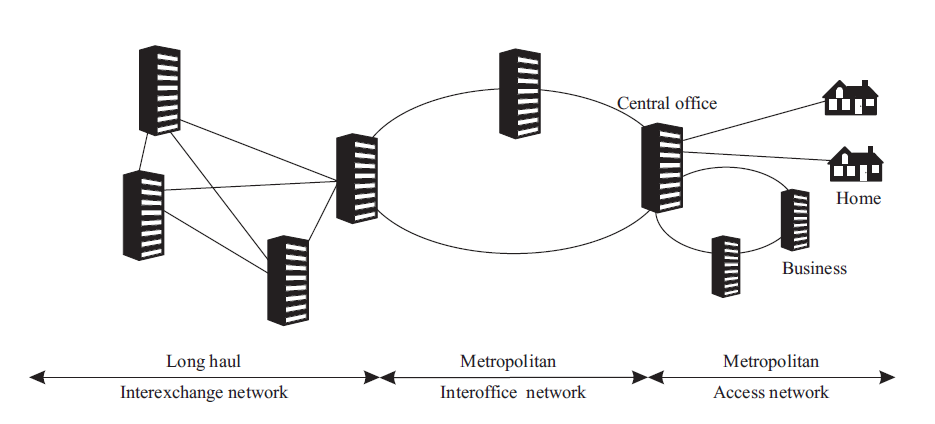
\includegraphics[width=330.8pt]{images/image2.png}
\end{center}
\end{frame}

\begin{frame}[shrink=10,t]{Παράδειγμα: Δίκτυο του ΟΤΕ}
\begin{center}
\setlength{\unitlength}{0.000038pt}
\begin{picture}(5672152,4844168)
\put(0,0){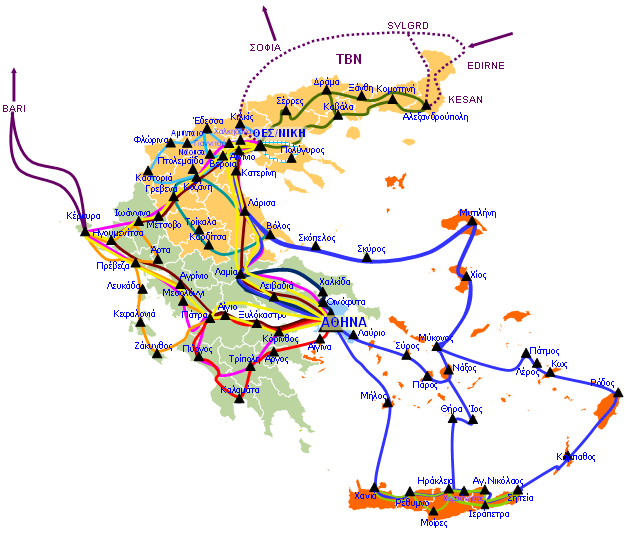
\includegraphics[width=213.1pt]{images/image3.png}}
\end{picture}
\end{center}
\centering\footnotesize Αποτελείται από διάφορους δακτυλίους που συνδέονται μεταξύ τους\par
\end{frame}

\begin{frame}[shrink=10,t]{Παράδειγμα Δικτύου: AT\&T}
\begin{center}
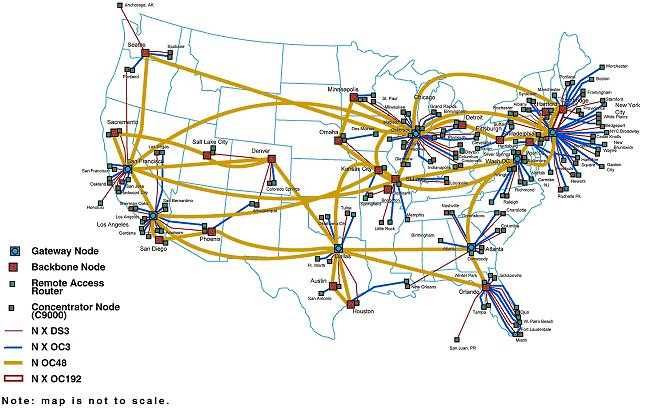
\includegraphics[width=306.9pt]{images/image4.jpeg}
\end{center}
\end{frame}

\begin{frame}[shrink=10,t]{Επίπεδα Δικτύου: Metropolitan (metro) και Long-Haul}
\begin{itemize}
\item \textbf{Metro}: To μέρος του δικτύου που εκτείνεται σε μία μεγάλη πόλη ή μία γεωγραφική περιοχή.
\item Το δίκτυο \textbf{access} είναι μέρος του metro και συνδέει  ένα central office στους πελάτες του δικτύου (οικιακοί χρήστες ή επιχειρήσεις). Καλύπτει μερικά χιλιόμετρα.
\item Το δίκτυο interoffice συνδέει τα central οffices μέσα στην ίδια γεωγραφική περιοχή. Εκτείνεται σε αποστάσεις μερικών δεκάδων χιλιομέτρων.
\item \textbf{Long-haul}: Συνδέει τα metro δίκτυα των διαφορετικών πόλεων και γεωγραφικών περιοχών. Εκτείνεται σε αποστάσεις από μερικές εκατοντάδες ως μερικές χιλιάδες(!) χιλιόμετρα.
\end{itemize}
\end{frame}

\begin{frame}[shrink=10,t]{Οι υπηρεσίες των παρόχων}
\begin{itemize}
\item \textit{Connection-oriented} (με σύνδεση):  Υπάρχει η έννοια της (σταθερής) σύνδεσης μεταξύ των μερών που μετέχουν στην επικοινωνία.
\item \textit{Circuit-switched}: Σε κάθε σύνδεση παρέχουμε σταθερό εύρος ζώνης.
\begin{itemize}
\item η σύνδεση (κύκλωμα) πρέπει να παραμένει ζωντανή εφόσον αρχικοποιηθεί
\item το άθροισμα του εύρος ζώνης όλων των κυκλωμάτων πρέπει να είναι μικρότερο από τη χωρητικότητα των συνδέσμων που χρησιμοποιούνται.
\item ρυθμοί κυκλωμάτων: από 64kb/s μέχρι μερικά Gb/s
\item παράδειγμα: PSTN (public switched telephone network) και μισθωμένες γραμμές (private lines).
\end{itemize}
\end{itemize}
\end{frame}

\begin{frame}[shrink=10,t]{Οι υπηρεσίες των παρόχων (2)}
\begin{itemize}
\item \textit{Packet Switching}: Χρησιμοποιείται ώστε να βελτιστοποιήσει την χρήση των πόρων (χωρητικότητα) όταν έχουμε bursty κίνηση.
\begin{itemize}
\item Τα δεδομένα χωρίζονται σε πακέτα και κάθε πακέτο μπορεί να πολυπλεχθεί με άλλα πακέτα άλλων δεδομένων.
\item \textit{Στατιστική πολυπλεξία (}\textit{Statistical Multiplexing)}: Όταν μία ζεύξη χρησιμοποιείται από πολλά ζευγάρια επικοινωνίας.
\item \textit{Datagram Service: }Τα πακέτα μπορεί να φτάνουν στον προορισμό τους από διαφορετικούς δρόμους
\item \textit{Frame Relay}: Εγγυόμαστε ένα μέσω bandwidth αλλά ο χρήστης μπορεί να “πιάσει” και παραπάνω από αυτό.
\end{itemize}
\end{itemize}
\end{frame}

\begin{frame}[shrink=10,t]{Είδη πολυπλεξίας δεδομένων (στο πεδίο του χρόνου)}
\begin{center}
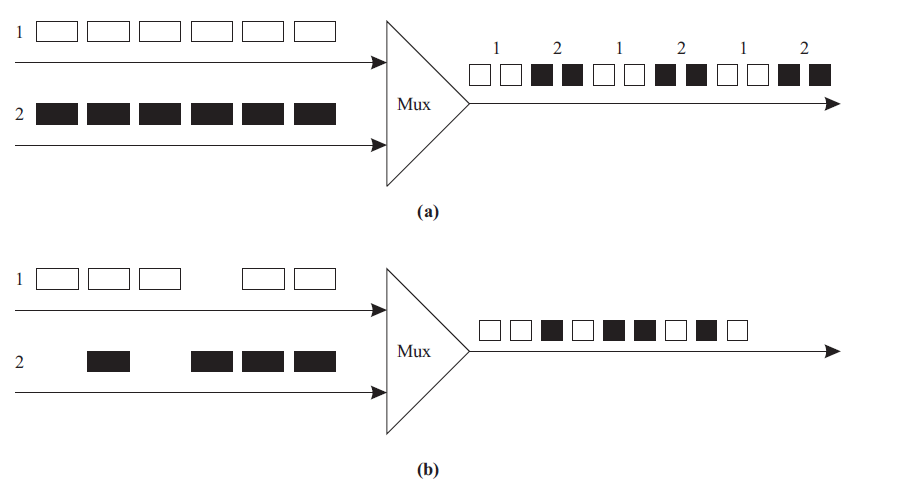
\includegraphics[width=357.8pt]{images/image5.png}
\end{center}
\end{frame}

\begin{frame}[t]{Οπτικά Δίκτυα}
\begin{itemize}
\item Πρώτης Γενιάς
\begin{itemize}
\item Οι οπτικές τεχνολογίες χρησιμοποιούνται για μετάδοση (οι ίνες απλά αντικαθιστούν το χαλκό).
\item Η επεξεργασία και η μεταγωγή (switching) γίνεται από τα ηλεκτρονικά κυκλώματα.
\item Παραδείγματα: SONET \& SDH
\end{itemize}
\item Δίκτυα Δεύτερης Γενιάς
\begin{itemize}
\item Γίνεται μία προσπάθεια η δρομολόγηση και η μεταγωγή να γίνουν στο οπτικό επίπεδο (optical layer).
\item Στην ουσία προσπαθούμε να κάνουμε τα οπτικά συστήματα… πιο έξυπνα!
\end{itemize}
\end{itemize}
\end{frame}

\begin{frame}[shrink=10,t]{Τρόποι Πολυπλεξίας (σε δίκτυα 2$^{\text{ης}}$ γενιάς)}
\begin{center}
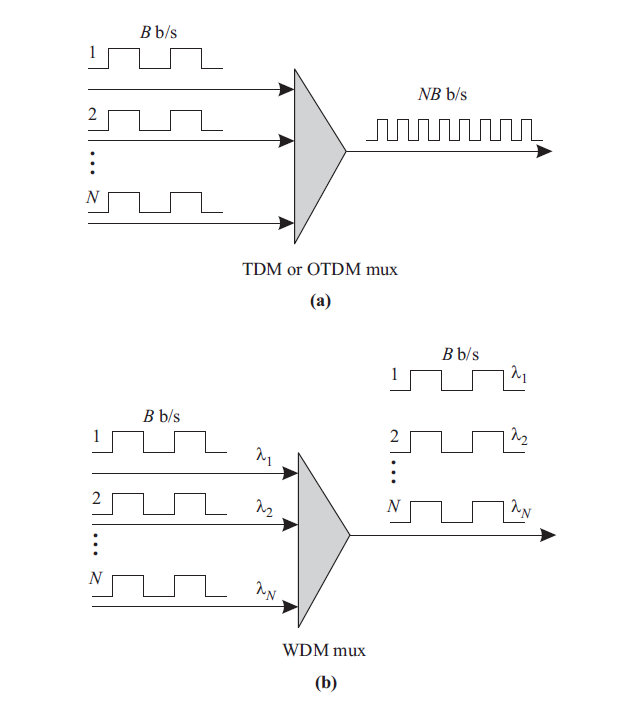
\includegraphics[width=171.6pt]{images/image6.png}
\end{center}
\end{frame}

\begin{frame}[shrink=10,t]{Time Domain Multiplexing (TDM)}
\begin{itemize}
\item H οπτική ίνα έχει \textbf{τεράστιο}\textbf{ }εύρος ζώνης που πρέπει να χρησιμοποιήσουμε όσο το δυνατόν καλύτερα
\item Ό ένας τρόπος είναι να αυξήσουμε το ρυθμό μετάδοσης πολυπλέκοντας πολλά μικρά “κανάλια”.
\item Π.χ. 64 κανάλια \ensuremath{\times} 155Μb/s = 10Gb/s
\item Εμπορικά διαθέσιμη ρυθμοί TDM είναι της τάξης των 40Gb/s.
\item Τα ηλεκτρονικά θέτουν ένα όριο στο μέγιστο ρυθμό.
\item Οι οπτικές τεχνολογίες για απευθείας TDM στο οπτικό επίπεδο (χωρίς ηλεκτρονικά) είναι ακόμα μακριά.
\end{itemize}
\end{frame}

\begin{frame}[t]{Wavelength Division Multiplexing (WDM)}
\begin{itemize}
\item Στην ουσία πρόκειται για πολυπλεξία στο πεδίο των συχνοτήτων.
\item Μεταδίδουμε πολλά μήκη κύματος στην ίδια ίνα και κάθε μήκος κύματος είναι μία ιδεατή ίνα (virtual fiber)
\item Σε μία πρώτη θεώρηση τα μήκη κύματος (χρώματα) δεν παρεμβάλλονται
\item Το WDM χρησιμοποιείται πολύ σε δίκτυα long-haul, metro αλλά και υποβρύχιες ζεύξεις.
\item Με χρήση TDM + WDM μπορούμε να μεταδώσουμε πληροφορία με ρυθμούς της τάξης του Tb/s (!) = 1.000Gb/s=1.000.000Mb/s
\end{itemize}
\end{frame}

\begin{frame}[shrink=20,t]{Δίκτυα Δεύτερης Γενιάς}
\begin{itemize}
\item Δίκτυο με δρομολόγηση μήκος κύματος (wavelength routing network)
\item To δίκτυο παρέχει lightpaths (οπτικές συνδέσεις σε ένα μήκος κύματος) στους χρήστες του
\item Χρήστες: τερματικά SONET ή IP routers.
\item Δυνατότητα αλλαγής μήκους κύματος κατά μήκος ενός lightpath
\item Επαναχρησιμοποίηση μήκους κύματος.
\end{itemize}
\medskip
\begin{itemize}
\item OADM=Optical add-drop multiplexer
\item OLT=Optical line terminals
\item OXC=Optical cross-connect
\end{itemize}
\begin{center}
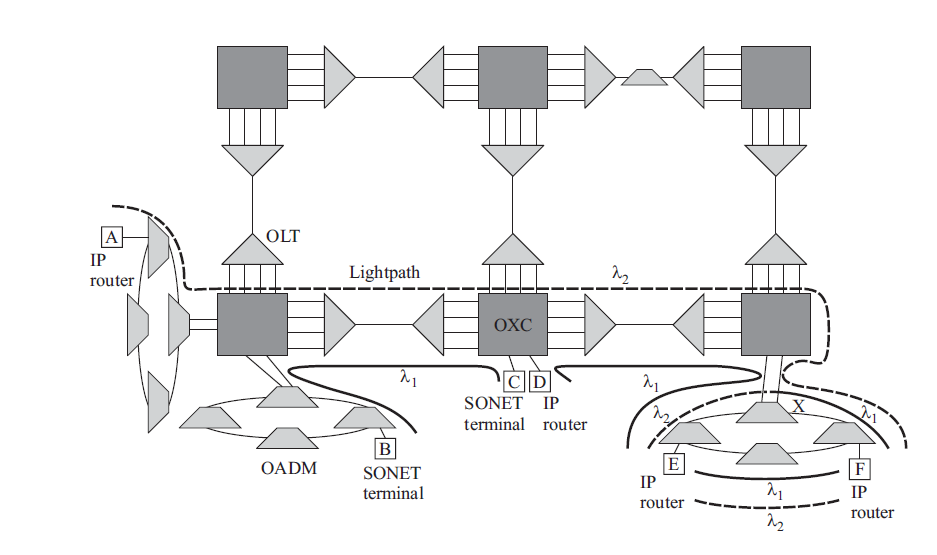
\includegraphics[width=233.8pt]{images/image7.png}
\end{center}
\end{frame}

\begin{frame}[shrink=20,t]{Δίκτυα Δεύτερης Γενιάς}
\begin{itemize}
\item ΟLT: πολυπλέκει και αποπολυπλέκει πολλά μήκη κύματος
\item OADM: Μπορεί να αφαιρέσει ή να προσθέσει σήματα στα διάφορα μήκη κύματος
\item OXC: Κάνει δρομολόγηση μήκους κύματος στις θύρες του.
\end{itemize}
\medskip
\begin{itemize}
\item OADM=Optical add-drop multiplexer
\item OLT=Optical line terminals
\item OXC=Optical cross-connect
\end{itemize}
\begin{center}
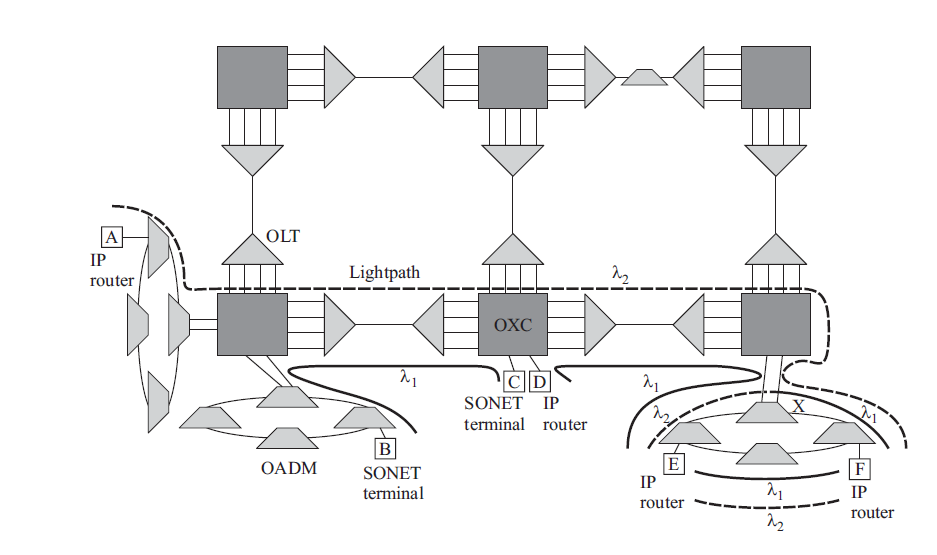
\includegraphics[width=233.8pt]{images/image7.png}
\end{center}
\end{frame}

\begin{frame}[shrink=20,t]{Περί στρωμάτων…}
\begin{itemize}
\item Η λειτουργικότητα των δικτύων μπορεί να κατανοηθεί καλύτερα αν τα χωρίσουμε σε στρώματα (ή επίπεδα -  layers).
\item Κάθε στρώμα εκτελεί ένα διακριτό ρόλο στο δίκτυο
\item Δεξιά φαίνεται η διαστρωμάτωση που έχει υιοθετηθεί σύμφωνα με το πρότυπο του OSI
\item Το πρότυπο αυτό είναι ωραίο στη θεωρία αλλά τι συμβαίνει στην πράξη;
\end{itemize}
\begin{center}
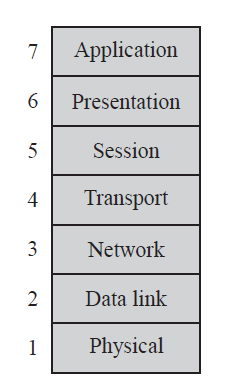
\includegraphics[width=89.6pt]{images/image8.png}
\end{center}
\end{frame}

\begin{frame}[shrink=20,t]{Παράδειγμα IP over SONET}
\begin{itemize}
\item Στο δίκτυο αυτό, το IP θεωρεί πως το SONET του προσφέρει μία πλειάδα από συνδέσεις από σημείο-προς-σημείο (point-to-point, PtP) μεταξύ των IP routers
\item To SONET ωστόσο έχει δικούς του μηχανισμούς δρομολόγησης και ως ένα σημείο περιλαμβάνει και αυτό στρώματα PHY, DLC και δικτύου.
\end{itemize}
\begin{center}
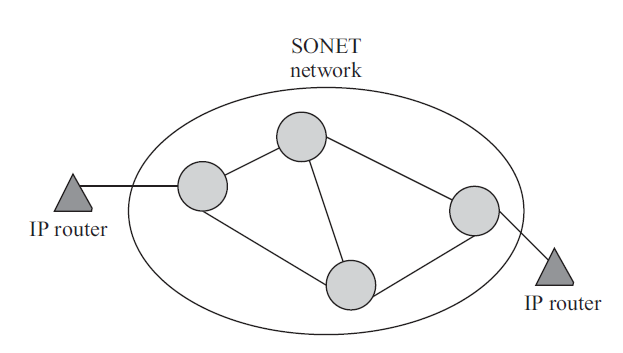
\includegraphics[width=197.5pt]{images/image9.png} 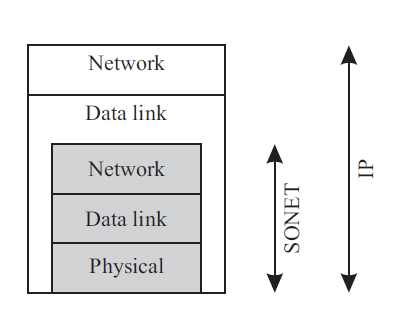
\includegraphics[width=140.8pt]{images/image10.png}
\end{center}
\end{frame}

\begin{frame}[shrink=20,t]{Το οπτικό στρώμα (optical layer)}
\begin{itemize}
\item Στα δίκτυα δεύτερης γενιάς υπάρχει και το οπτικό στρώμα (optical layer).
\item Παρέχει υπηρεσίες σε άλλα στρώματα και προσαρμόζεται σε διάφορα ανώτερα στρώματα.
\item Η ακραία περίπτωση είναι το optical layer να παρέχει και packet switching είτε σε επίπεδο virtual circuits είτε σε datagram (Θα το δούμε ποτέ?)
\end{itemize}
\begin{center}
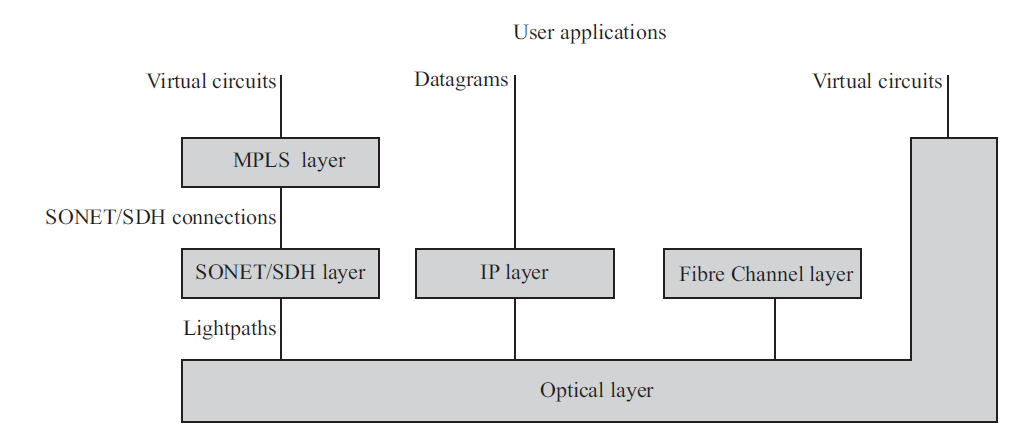
\includegraphics[width=338.3pt]{images/image11.png}
\end{center}
\end{frame}

\begin{frame}[t]{Το οπτικό στρώμα (optical layer)}
\begin{itemize}
\item Το οπτικό στρώμα παρέχει lightpaths στα ανώτερα στρώματα.
\item Τα lightpaths αυτά είναι για τα ανώτερα στρώματα ιδεατές οπτικές ίνες.
\item Μπορούν να μεταδώσουν ρυθμούς της τάξης των 10Gb/s-40Gb/s
\item Ανάλογα με τις δυνατότητες του δικτύου, τα lightpaths μπορεί να είναι μόνιμα ή να μπορούν να αλλάξουν (circuit-switched).
\item Στο παρελθόν (αλλά πολλές φορές ακόμα και τώρα!) τον ρόλο του οπτικού στρώματος τον έπαιζε το SONET/SDH.
\end{itemize}
\end{frame}

\begin{frame}[t]{Επίπεδο Διαφάνειας (Transparency)}
\begin{itemize}
\item Το οπτικό στρώμα παρέχει τα lightpaths τα οποία είναι διαφανή στο χρήστη.
\item Με τον όρο διαφανή εννοούμε πως μπορούν να μεταφέρουν οποιοδήποτε (σχεδόν!) τύπο δεδομένων ανεξαρτήτως πρωτοκόλλου, ψηφιακής ή αναλογικής μορφής, κτλ
\item Απλά ορίζεται ένας ελάχιστος και ένας μέγιστος ρυθμός μετάδοσης
\item Επομένως ένας πάροχος μπορεί να χρησιμοποιήσει την ίδια υποδομή για να παρέχει πολλές υπηρεσίες.
\end{itemize}
\end{frame}

\begin{frame}[shrink=20,t]{Βασικές Παράμετροι Οπτικών Σημάτων}
\begin{itemize}
\item Το φως που διαδίδεται μέσα σε μία οπτική ίνα χαρακτηρίζεται από το μήκος κύματος του.
\item Το μήκος κύματος \textit{λ} συνδέεται με την συχνότητα του κύματος \textit{f}.
\item To \textit{λ} και το \textit{f} χαρακτηρίζουν \textbf{το οπτικό φέρον }το οποίο είναι το Η/Μ πεδίο που εκπέμπεται από ένα αδιαμόρφωτο laser
\item Σε μία πρώτη προσέγγιση (πολύ πρώτη!) το ηλεκτρικό πεδίο του φέροντος έχει το μορφή \textit{Α}cos(2π\textit{ft}) δηλαδή περιέχει δύο συχνότητες τις \ensuremath{\pm}\textit{f}
\item Στον ελεύθερο χώρο το ηλεκτρικό αυτό πεδίο διαδίδεται ως \textit{A}(\textit{d})cos(2π\textit{ft}-\textit{kz}) όπου \textit{d} είναι η απόσταση που έχει καλύψει
\item το \textit{k}=2π/\textit{λ }είναι το κυματάνυσμα του κύματος (θυμηθείτε το μάθημα της Διάδοσης).
\end{itemize}
\end{frame}

\begin{frame}[shrink=10,t]{Βασικές Παράμετροι Οπτικών Σημάτων}
\begin{itemize}
\item Στην περίπτωση των σημάτων WDM χρησιμοποιούμε το μήκος κύματος \textit{λ} το οποίο σχετίζεται με την (φέρουσα) συχνότητα \textit{f} του σήματος βάση της σχέσης \textit{λ}=\textit{c}/\textit{f.}
\item Στην παραπάνω σχέση, \textit{c}=3\ensuremath{\times}10$^{8}$m/s είναι η ταχύτητα του φωτός στο κενό.
\item Μπορούμε να υπολογίσουμε την απόσταση Δ\textit{λ} δύο σημάτων ως προς το μήκος κύματος αν γνωρίζουμε την συχνοτική απόσταση Δ\textit{f }μέσω της σχέση Δ\textit{f}=(-\textit{c}/\textit{λ}$^{\text{2}}$)Δλ.
\item Έτσι γύρω από το λ=1550nm, ένα συχνοτικό spacing 100GHz αντιστοιχεί σε μία απόσταση 0.8nm
\end{itemize}
\end{frame}

\begin{frame}[shrink=10,t]{Βασικές Παράμετροι Οπτικών Σημάτων}
\begin{center}
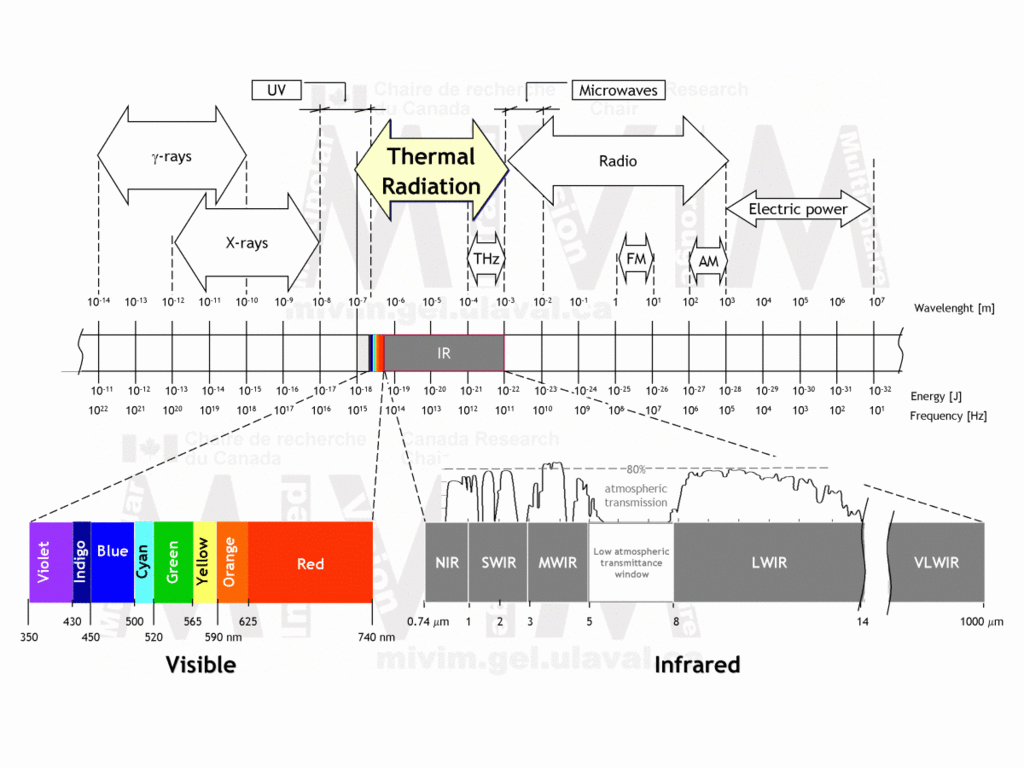
\includegraphics[width=260.0pt]{images/image12.png}
\end{center}
\end{frame}

\begin{frame}[shrink=10,t]{Βασικές Παράμετροι Οπτικών Σημάτων}
\begin{itemize}
\item Στο φέρον αποτυπώνουμε την πληροφορία μας
\item Π.χ. αν \textit{x}(\textit{t}) είναι το σήμα που θέλουμε να μεταδώσουμε τότε μπορούμε να “αναγκάσουμε” το laser να εκπέμπει το πεδίο\textit{ Α}\textit{x}(\textit{t})cos(2π\textit{ft})
\item H παραπάνω περίπτωση είναι φυσικά η διαμόρφωση κατά πλάτος
\item Ως αποτέλεσμα της διαμόρφωσης του σήμα πλέον καταλαμβάνει πολλές συχνότητες
\item Εύρος ζώνης είναι η συχνοτική περιοχή που καταλαμβάνει το σήμα γύρω από την κεντρική συχνότητα \textit{f}
\item Στις οπτικές επικοινωνίες χρησιμοποιούνται σχετικές απλές μέθοδοι διαμόρφωσης με φασματική απόδοση 0.4bit/s/Hz.
\item Έτσι ένα σήμα 10Gb/s καταλαμβάνει ένα εύρος ζώνης περίπου 25GHz
\end{itemize}
\end{frame}

\begin{frame}[shrink=10,t]{Πρότυπα Μήκους Κύματος}
\begin{center}
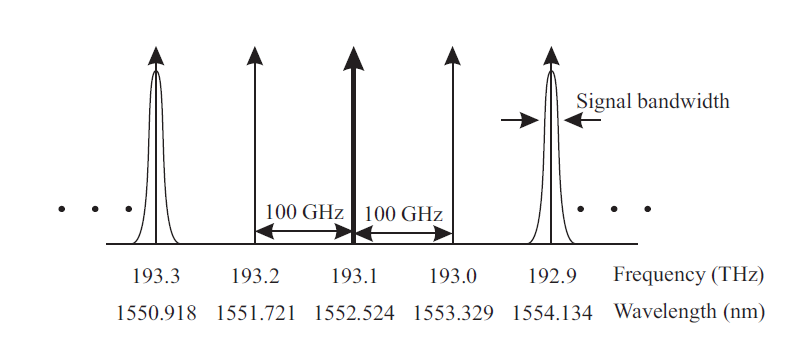
\includegraphics[width=378.1pt]{images/image13.png}
\end{center}
\end{frame}

\begin{frame}[t]{Ισχύς Σήματος}
\begin{itemize}
\item Η ισχύς του σήματος είναι και αυτή μία πολύ βασική παράμετρος
\item Καθορίζει σε μεγάλο βαθμό τις επιδόσεις ενός συστήματος οπτικών επικοινωνιών
\item Η ισχύς υπολογίζεται από το επιφανειακό ολοκλήρωμα του διανύσματος Poynting \ensuremath{\tfrac{1}{2}}Re\{\textbf{Ε}\textbf{\ensuremath{\times}Η*}\}\textbf{.}
\item Εκφράζει το ρυθμό μεταβολής της ενέργειας του κύματος που περνάει από μία σταθερή διατομή
\item Μετριέται συνήθως mW ή dBm
\end{itemize}
\end{frame}

\begin{frame}[t]{Πόλωση του Φωτός}
\begin{itemize}
\item Όταν το φως διαδίδεται κατά τον άξονα z είδαμε στο μάθημα της διάδοσης ότι το ηλεκτρικό πεδίο έχει δύο συνιστώσες: \textit{E}$_{\text{\textit{x}}}$ και \textit{E}$_{\text{\textit{y}}}$.
\item Ανάλογα με την κίνηση που εκτελεί το άκρο του διανύσματος \textbf{E}=(\textit{E}$_{\text{\textit{x}}}$,\textit{E}$_{\text{\textit{y}}}$) με την πάροδο του χρόνου ορίζεται η πόλωση του φωτός.
\item Η πόλωση μπορεί να είναι:
\begin{itemize}
\item γραμμική
\item κυκλική
\item ελλειπτική
\end{itemize}
\end{itemize}
\end{frame}

\begin{frame}[shrink=10,t]{Πόλωση του Φωτός}
\begin{itemize}
\item Γιατί η πόλωση είναι σημαντική;
\item Επειδή διάφορα στοιχεία του δικτύου αντιδρούν διαφορετικά ότι π.χ. το φως είναι πολωμένο γραμμικά ως προς \textit{x} (\textit{E}$_{\text{\textit{y}}}$=0) και διαφορετικά ως προς \textit{y} (\textit{E}$_{\text{\textit{x}}}$=0)
\item Το παραπάνω φαινόμενο λέγεται \textit{διπλοδιαθλαστικότητα}.
\item Επομένως έχει σημασία να γνωρίζουμε την κατάσταση της πόλωσης ή να φροντίζουμε ώστε τα δομικά στοιχεία που χρησιμοποιούμε να είναι \textit{αναίσθητα στην πόλωση.}
\end{itemize}
\end{frame}

\begin{frame}[t]{Κβαντική Φύση του Φωτός}
\begin{itemize}
\item Το φως είναι κύμα ή σωματίδια;
\item Η πιο σωστή περιγραφή είναι ότι είναι σωματίδια που ονομάζονται \textit{φωτόνια.}
\item Τα φωτόνια είναι στην ουσία φορείς του πεδίου που μεταφέρουν τη δράση του.
\item Μία οπτική δέσμη αποτελείται από πολλά φωτόνια.
\item Η ενέργεια του φωτονίου \textit{E} συνδέεται με την συχνότητα του κύματος, \textit{Ε}=\textit{hf}.
\item \textit{h} είναι η σταθερά του Planck, \textit{h}=6.626\ensuremath{\times}10$^{-34}$ m$^{\text{2}}$ kg/s.
\end{itemize}
\end{frame}

\begin{frame}[shrink=20,t]{Σύμφωνο και Ασύμφωνο Φως}
\begin{itemize}
\item Στις περισσότερες περιπτώσεις η ισχύς του σήματος \textit{P} είναι απλά ανάλογη του μέτρου στο τετράγωνο του πλάτους του ηλεκτρικού πεδίου \textit{Ε}, \textit{P}\textasciitilde{}|\textit{E}|$^{\text{2}}$.
\item Όταν έχουμε παραπάνω από ένα πεδία η συνολική ισχύς είναι \textit{P}\textasciitilde{}|\textit{E}$_{\text{1}}$+\textit{E}$_{\text{2}}$|$^{\text{2}}$.
\item H συνολική ισχύς καθορίζεται από την διαφορά φάσης των δύο πεδίων
\begin{itemize}
\item \textit{P}\textasciitilde{}|\textit{E}$_{\text{1}}$+\textit{E}$_{\text{2}}$|$^{\text{2}}$=|\textit{Α}exp(\textit{j}\textit{φ}$_{\text{1}}$)+ \textit{Α}exp(\textit{j}\textit{φ}$_{\text{2}}$)|$^{\text{2}}$=2\textit{A}$^{\text{2}}$+2\textit{A}$^{\text{2}}$cos(\textit{φ}$_{\text{1}}$-\textit{φ}$_{\text{2}}$).
\end{itemize}
\end{itemize}
\end{frame}

\begin{frame}[shrink=20,t]{Σύμφωνο και Ασύμφωνο Φως}
\begin{itemize}
\item \textit{Σύμφωνο} είναι το φως το οποίο αποτελείται από συνιστώσες που έχουν πολύ καλά ορισμένη διαφορά φάσης.
\item \textit{Ασύμφωνο} είναι το φως το οποίο αποτελείται από συνιστώσες που έχουν τυχαία διαφορά φάσης.
\item Στο ασύμφωνο φως δεν υπάρχει συμβολή
\begin{itemize}
\item Αν οι συνιστώσες \textit{Ν} είναι πολλές
\item \textit{P}\textasciitilde{}|\ensuremath{\infty}$_{\text{\textit{p}}}$\textit{E}$_{\text{\textit{p}}}$|$^{\text{2}}$=|\ensuremath{\infty}$_{\text{\textit{p}}}$\textit{Α}exp(\textit{j}\textit{φ}$_{\text{\textit{p}}}$)|$^{\text{2}}$=\textit{A}$^{\text{2}}$Σ$_{\text{\textit{pq}}}$exp(\textit{j}(\textit{φ}$_{\text{\textit{p}}}$-\textit{φ}$_{\text{\textit{q}}}$))\ensuremath{>}\textit{Ν}$^{\text{2}}$\textit{Α}$^{\text{2}}$<exp(\textit{j}(\textit{φ}-\textit{φ}’))>\textit{ΝΑ}$^{\text{2}}$=\ensuremath{\infty}$_{\text{\textit{p}}}$|\textit{E}$_{\text{\textit{p}}}$|$^{\text{2}}$
\item Δηλαδή η συνολική ισχύς είναι απλά το άθροισμα της ισχύος των επιμέρους συνιστωσών.
\end{itemize}
\end{itemize}
\end{frame}

\begin{frame}[shrink=10,t]{Σύμφωνο και Ασύμφωνο Φως}
\begin{itemize}
\item Η συμφωνία μπορεί να είναι επίσης
\begin{itemize}
\item συχνότητας
\item χωρική
\end{itemize}
\item Μπορούμε να σκεφτόμαστε το σύμφωνο φως ως το φως που παράγεται από μία πολύ μικρή (σημειακή πηγή).
\end{itemize}
\begin{center}

\includegraphics[width=220.6pt]{images/image14.png} 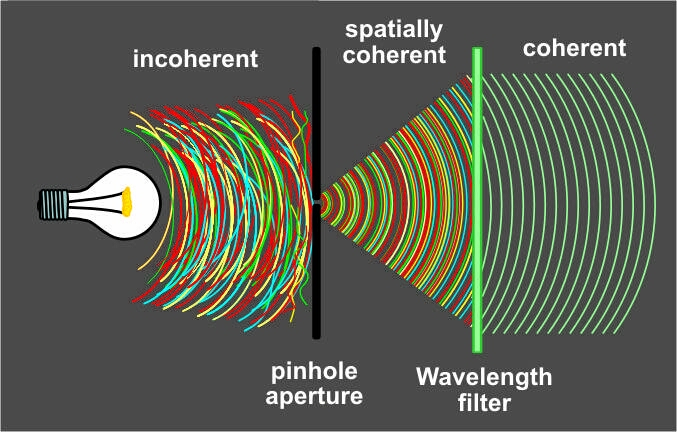
\includegraphics[width=117.7pt]{images/image15.jpeg}
\end{center}
\end{frame}

\begin{frame}[shrink=20,t]{Μulti mode και Single mode ίνες}
\begin{itemize}
\item Σε μία πρώτη προσέγγιση η διάδοση σημάτων στην οπτική ίνα μπορεί να περιγραφτεί με την γεωμετρική οπτική.
\item Οι οπτικές ακτίνες που ανακλώνται ολικά στα “τοιχώματα” αποτελούν τους τρόπους διάδοσης
\item Υπάρχουν ίνες που υποστηρίζουν πολλούς τρόπους διάδοσης (multimode) ή ίνες που υποστηρίζουν έναν τρόπο διάδοσης (single mode).
\end{itemize}
\begin{center}
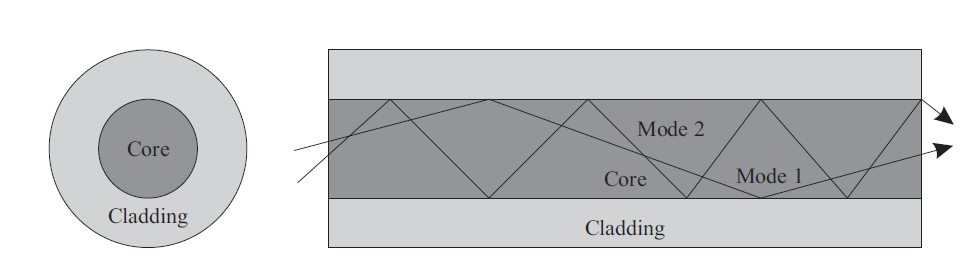
\includegraphics[width=338.3pt]{images/image16.png}
\end{center}
\end{frame}

\begin{frame}[shrink=10,t]{Στάδια Εξέλιξης Οπτικών Δικτύων}
\begin{center}
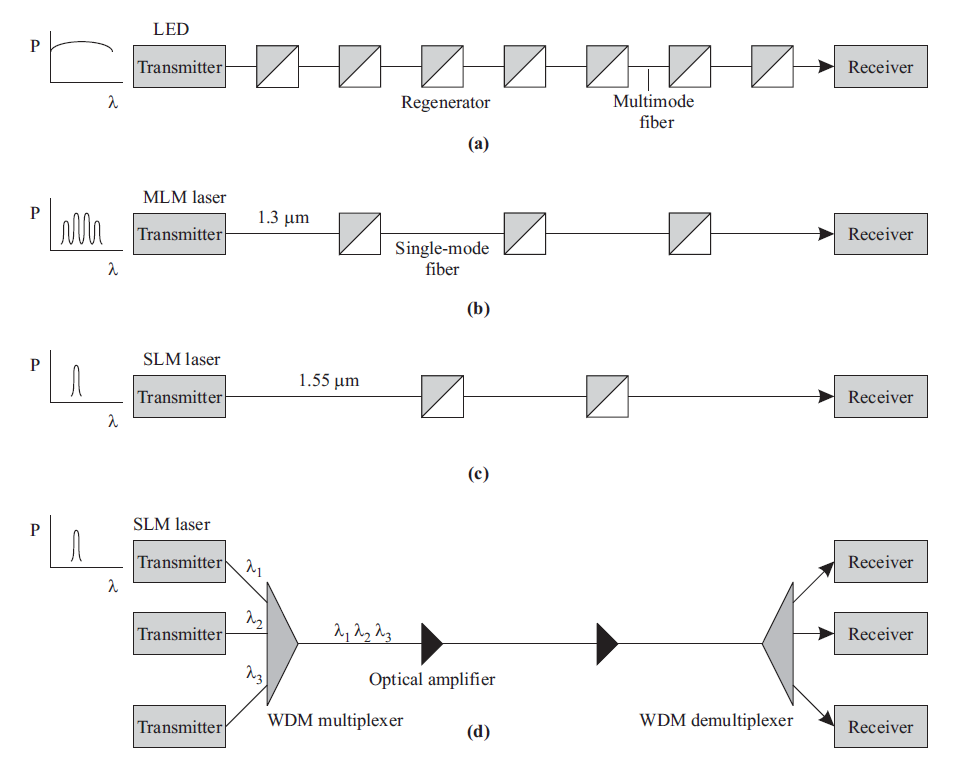
\includegraphics[width=243.8pt]{images/image17.png}
\end{center}
\end{frame}

\begin{frame}[shrink=20,t]{Λίγη Ιστορία}
\begin{itemize}
\item τέλη 1970- αρχές 1980: multimode ίνες και LEDs ή LASERs με πολλούς τρόπους
\begin{itemize}
\item εμβέλεια: μερικά χιλιόμετρα
\item κακή χρήση του φάσματος (πηγές με ευρύ φάσμα)
\item υψηλές απώλειες (μήκη κύματος στα 0.8μm ή 1.3μm)
\item Πολλοί τρόποι διάδοσης σημαίνει διεύρυνση παλμών (ISI)
\item Χρήση αναγεννητών κάθε 10km
\item Ρυθμοί από 32 εώς 140Mb/s
\end{itemize}
\item το 1984 άρχισαν να εγκαθίστανται single mode ίνες
\begin{itemize}
\item Πολύτροπα laser στο 1.3μm (εξαλείφεται ένα είδος διασποράς όπως θα δούμε παρακάτω).
\item Διάμετρος πυρήνα ίνας 8μm-10μm.
\item Αναγεννητές κάθε 40km
\item Ρυθμοί: μερικές εκατοντάδες Mb/s
\end{itemize}
\end{itemize}
\end{frame}

\begin{frame}[shrink=20,t]{Λίγη Ιστορία}
\begin{itemize}
\item Τέλη δεκαετίας 1980: Χρήση πηγών με μήκος κύματος εκπομπής στα 1.55μm.
\begin{itemize}
\item Ελαχιστοποίηση απωλειών
\item Η διασπορά (dispersion) όμως προκαλεί ISI
\item Εγκατάσταση ινών dispersion shifted όπου έχουν μικρή διασπορά στα 1.55μm (MCI-Verizon, NTT, κτλ)
\item Distributed feedback lasers (DFB): Μικρότερο φάσμα εκπομπής (μονότροπα laser)
\item Ρυθμοί της τάξης του 1Gb/s
\end{itemize}
\item Αρχές της δεκαετίας του 1990: Οπτικοί Ενισχυτές
\begin{itemize}
\item EDFA: Erbium Doped Fiber Amplifier, παρέχουν (αμιγώς) οπτική ενίσχυση στο 1.55μm.
\item Καταλύτης για την εγκατάσταση συστημάτων WDM
\item Ρυθμοί μετάδοσης (ανά κανάλι): 10Gb/s
\item Απόσταση ενισχυτών: 40-80km
\item Χρήση εξωτερικών διαμορφωτών για περαιτέρω βελτιστοποίηση του φάσματος.
\end{itemize}
\end{itemize}
\end{frame}

\begin{frame}[shrink=10,t]{Λίγη Ιστορία}
\begin{itemize}
\item H ανάπτυξη τεχνικών αντιστάθμισης διασποράς (dispersion compensation) επέτρεψε την άνετη μετάδοση με ρυθμούς 10Gb/s
\item Ωστόσο όσο αυξάνονται οι ρυθμοί μετάδοσης αρχίζουν να παίζουν ρόλο κάποια άλλα φαινόμενα
\begin{itemize}
\item Μη γραμμική παραμόρφωση (π.χ. four wave mixing – FWM)
\item Φαινόμενα πόλωσης
\item Μη ομαλή απόκριση των EDFA ως προς την συχνότητα
\end{itemize}
\item Αναπτύχθηκαν ίνες που είχανε μικρότερη διασπορά από τις συμβατικές και ήτανε ειδικά σχεδιασμένες για να προκαλούν μικρότερη μη γραμμική παραμόρφωση.
\item Σήμερα
\begin{itemize}
\item ρυθμοί μετάδοσης ανά κανάλι: 10-40Gb/s
\item συνολική χωρητικότητα: 10Τb/s
\item απόσταση καναλιών: 50GHz
\item αποστάσεις μετάδοσης μέχρι και μερικές εκατοντάδες χιλιόμετρα χωρίς ανάγκη ηλεκτροοπτικής αναγέννησης
\end{itemize}
\end{itemize}
\end{frame}

\begin{frame}[shrink=10,t]{Μπάντες (συχνοτικές ζώνες) μετάδοσης}
\begin{center}
\setlength{\unitlength}{0.000053pt}
\begin{picture}(6772275,2657475)
\put(0,0){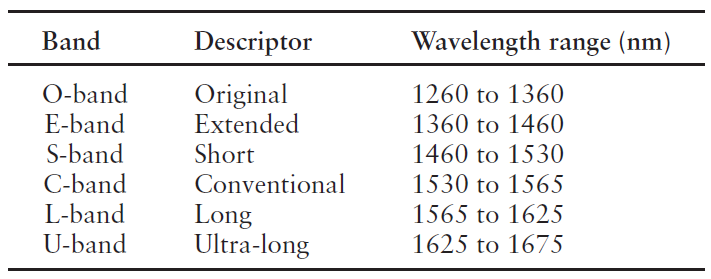
\includegraphics[width=358.2pt]{images/image18.png}}
\put(5913810,602216){\footnotesize \shortstack{EDFA}}
\put(5945342,102150){\footnotesize \shortstack{Raman?}}
\put(5945342,1030844){\footnotesize \shortstack{Raman?}}
\end{picture}
\end{center}
\end{frame}

\section[Οπτικές Ίνες]{Μέρος 2$^{\text{ο}}$: Οπτικές Ίνες}
\begin{frame}
\vfill
\begin{center}
{\Large\structure{Μέρος 2$^{\text{ο}}$: Οπτικές Ίνες}}
\end{center}
\vfill
\end{frame}

\begin{frame}[t]{Οπτική ίνες}
\begin{itemize}
\item Η οπτική ίνα μπορεί να υποστηρίξει ένα εύρος ζώνης \ensuremath{\ge}25ΤΗz με πολύ χαμηλές απώλειες
\begin{itemize}
\item \textasciitilde{}10$^{8}$ τηλεφωνικές συνδιαλέξεις(!)
\item 10$^{6}$ κανάλια HDTV
\end{itemize}
\item Ωστόσο η ίνα θέτει διάφορους φυσικούς περιορισμούς που πρέπει να λαμβάνονται υπόψη κατά τον σχεδιασμό:
\begin{itemize}
\item απώλειες
\item διασπορά
\item μη γραμμικά φαινόμενα
\end{itemize}
\end{itemize}
\end{frame}

\begin{frame}[shrink=10,t]{Εγκατάσταση Οπτικών Ινών}
\begin{itemize}
\item Η εγκατάσταση των οπτικών καλωδίων είναι αρκετά χρονοβόρα διαδικασία
\begin{itemize}
\item Σχεδιασμός (όδευση)
\item Προγραμματισμός και Π/Υ
\item Εγκρίσεις από Δήμο και ΕΕΤΤ
\item Δημόσια Έργα (σκάψιμο)
\item Τοποθέτηση καλωδίων (Φύσημα)
\item Τερματισμός καλωδίων
\item Δοκιμή Ζεύξης
\item Συντήρηση!
\end{itemize}
\end{itemize}
\end{frame}

\begin{frame}[shrink=20,t]{Σχεδιασμός (Όδευση)}
\begin{itemize}
\item Ο πιο φθηνός τρόπος δεν είναι ο συντομότερος!
\item Π.χ. ενώ η ευθεία απόσταση μεταξύ των κτιρίων του Χαροκοπείου είναι \textasciitilde{}700μ το συνολικό μήκος ίνας είναι 1500μ.
\begin{itemize}
\item Δεν μπορούμε εύκολα να περάσουμε από τις γραμμές του τρένου
\item Δεν μπορούμε να περάσουμε πάνω από γέφυρες
\item Αποφεύγουμε πεζόδρομους
\item Προτιμούμε να σκάψουμε σε άσφαλτο
\item Οι δήμοι μπορεί να έχουν διαφορετικές απαιτήσεις για αποκατάσταση του οδοστρώματος (φρεζάρισμα, κτλ).
\end{itemize}
\end{itemize}
\begin{center}
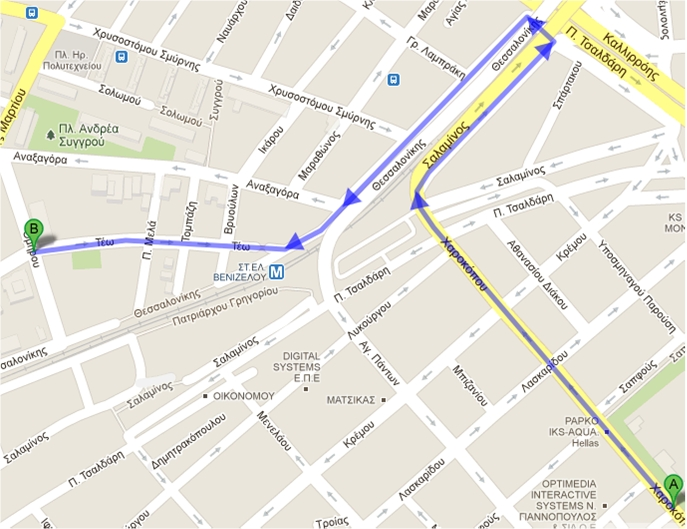
\includegraphics[width=172.5pt]{images/image19.jpeg} 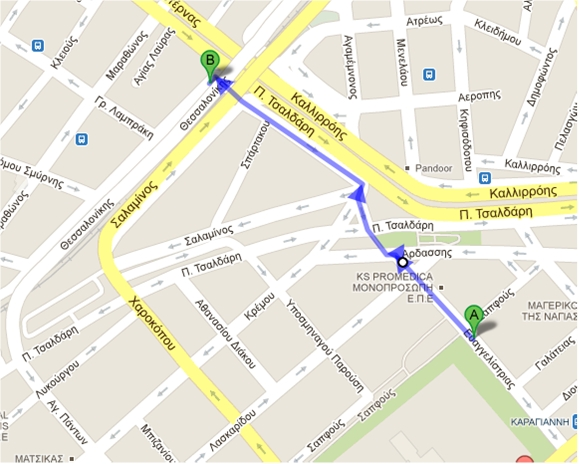
\includegraphics[width=165.8pt]{images/image20.jpeg}
\end{center}
\end{frame}

\begin{frame}[t]{Προϋπολογισμός}
\begin{itemize}
\item Θα πρέπει να ληφθούν υπόψη
\begin{itemize}
\item Κόστη έργων μαζί με αποκατάσταση οδοστρώματος!
\item Κόστη πολυσωλήνα, καλωδίων και patch panels
\item Προδιαγραφές χάνδακα (π.χ. 80mm πλάτος, 400mm βάθος)
\item Πλήθος Φρεατίων
\item Υπηρεσίες Διακρίβωσης
\item Υπηρεσίες Συντήρησης
\end{itemize}
\item Πρώτη εκτίμηση κόστους σε αστική περιοχή: \textasciitilde{}30 ευρώ το μέτρο.
\end{itemize}
\end{frame}

\begin{frame}[shrink=20,t]{Σκάψιμο}
\begin{itemize}
\item Σε αστική περιοχή ο ρυθμός σκαψίματος είναι περίπου 700μ την ημέρα
\item Χρειάζεται ιδιαίτερη προσοχή διότι μπορεί να υπάρχουν και άλλα δίκτυα στην περιοχή: νερού, ηλεκτρικού και οπτικής ίνας.
\item Συνήθως δεν υπάρχουν ακριβή σχέδια…
\end{itemize}
\begin{center}
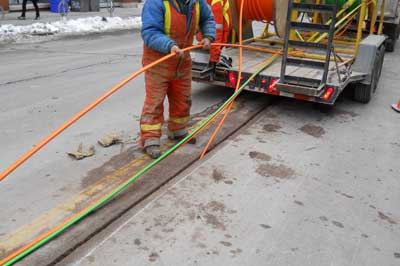
\includegraphics[width=202.2pt]{images/image21.jpeg} 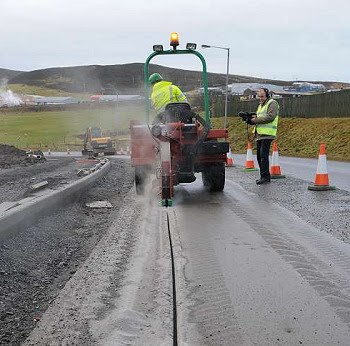
\includegraphics[width=136.1pt]{images/image22.jpeg}
\end{center}
\end{frame}

\begin{frame}[shrink=20,t]{Τερματισμός}
\begin{itemize}
\item Ο τερματισμός της ίνας γίνεται με τους οπτικούς κατανεμητές (optical patch panel)
\item Στην ουσία “ξεχωρίζουμε” τις ίνες οι οποίες υπάρχουν μέσα στο καλώδιο οπτικής ίνας.
\item Στο patch panel μπορούμε να συνδέσουμε μικρές ίνες (patch cords) και από εκεί και πέρα να συνδέσουμε τo switch.
\end{itemize}
\begin{center}
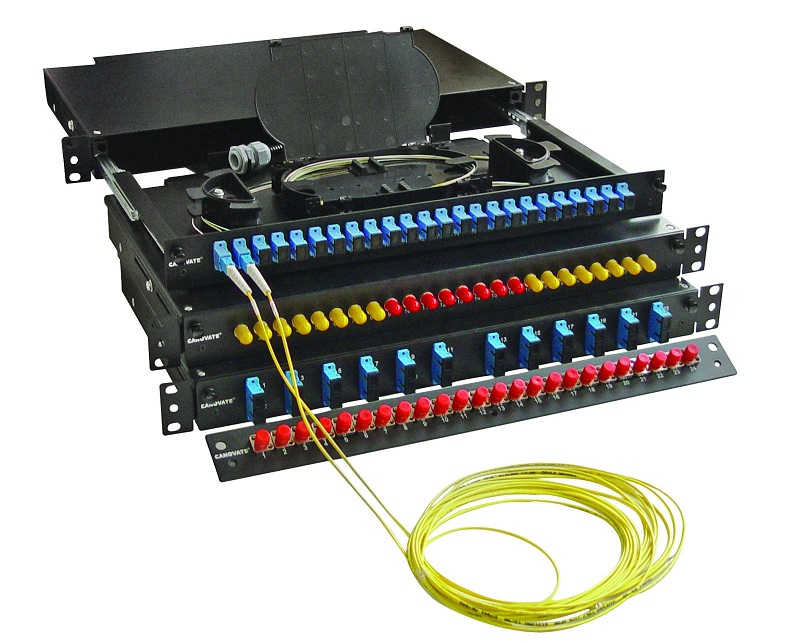
\includegraphics[width=186.7pt]{images/image23.jpeg}
\end{center}
\end{frame}

\begin{frame}[shrink=10,t]{Τερματισμός – Είδη connector}
\begin{center}
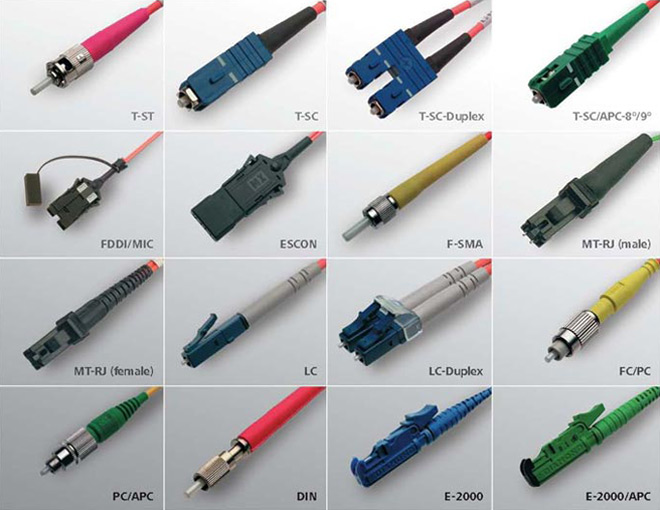
\includegraphics[width=252.4pt]{images/image24.jpeg}
\end{center}
\end{frame}

\begin{frame}[shrink=20,t]{Απώλειες}
\begin{itemize}
\item Ακολουθούν έναν εκθετικό νόμο, \textit{P}$_{\text{out}}$=\textit{P}$_{\text{in}}$\textit{e}$^{\text{\textit{aL}}}$
\item χαρακτηρίζονται από τον συντελεστή \textit{a}$_{\text{dB}}$ που μετριέται σε dB/Km.
\end{itemize}
\begin{center}
$\displaystyle \begin{aligned}a(\mathrm{dB/km})&\equiv 10\log_{10}(\text{Loss per unit distance})\\&=-\frac{10}{L}\log_{10}\left(\frac{P_{\mathrm{out}}}{P_{\mathrm{in}}}\right)=(10\log_{10}e)\,a=4.343\,a\end{aligned}$\\[0.6ex]
\end{center}
\end{frame}

\begin{frame}[shrink=20,t]{Αιτίες Απωλειών}
\begin{itemize}
\item Δύο είναι οι κυριότερες αιτίες απωλειών στις οπτικές ίνες
\begin{itemize}
\item Απορρόφηση υλικού (πολύ μικρή για το SiO$_{\text{2}}$)
\item Απορρόφηση λόγω νοθεύσεων του κρυστάλλου.
\item Σκέδαση Rayleigh (o κύριος λόγος των απωλειών στις οπτικές ίνες).
\item Η σκέδαση Rayleigh συμβαίνει όταν το μήκος κύματος του φωτός είναι πολύ μεγαλύτερο από την ανομοιογένεια στην οποία σκεδάζεται.
\item 2.5dB/Km στα 0.8μm
\item 0.4dB/Km στα 1.3μm
\item 0.25dB/Km στα 1.55μm
\item Aπώλειες κάμψεων (ακτίνα καμπυλότητας πρέπει να είναι μεγαλύτερη από μερικά cm)
\end{itemize}
\end{itemize}
\begin{center}
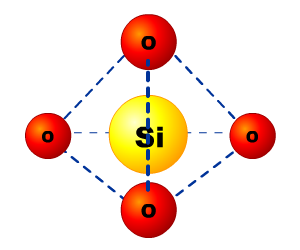
\includegraphics[width=97.4pt]{images/image26.png} 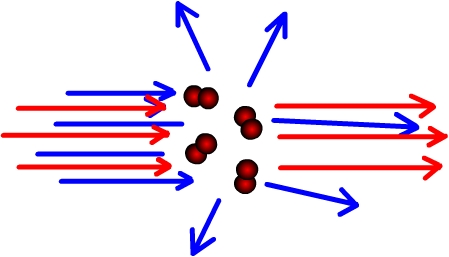
\includegraphics[width=141.9pt]{images/image27.jpeg} 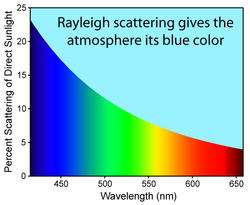
\includegraphics[width=99.0pt]{images/image28.png}
\end{center}
\end{frame}

\begin{frame}[shrink=10,t]{Αιτίες Απωλειών}
\begin{center}
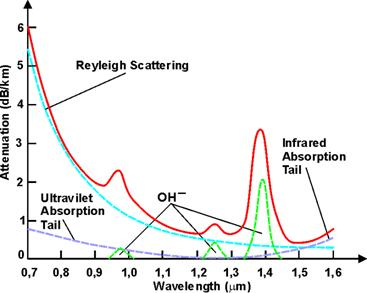
\includegraphics[width=244.2pt]{images/image29.jpeg}
\end{center}
\end{frame}

\begin{frame}[shrink=10,t]{Απώλειες Κάμψης}
\begin{center}
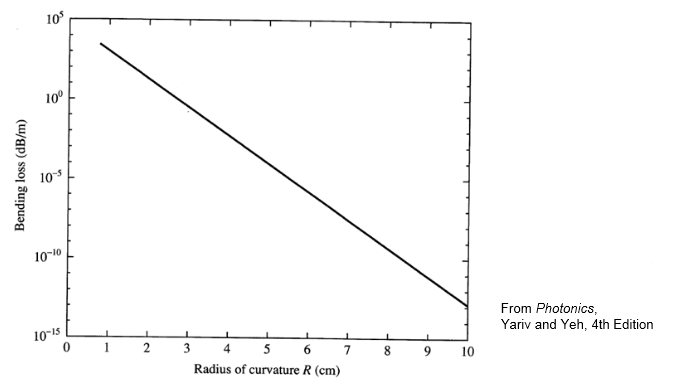
\includegraphics[width=348.5pt]{images/image30.png}
\end{center}
\end{frame}

\begin{frame}[shrink=10,t]{Εξάρτηση Απωλειών από την Συχνότητα}
\begin{center}
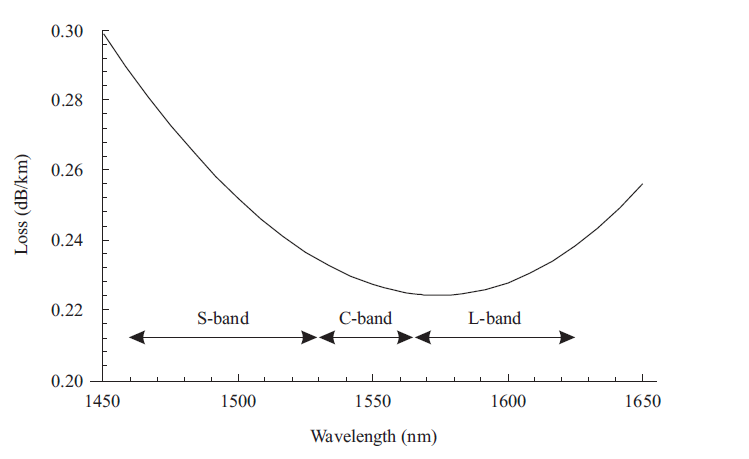
\includegraphics[width=295.8pt]{images/image32.png}
\end{center}
\end{frame}

\begin{frame}[shrink=20,t]{Διασπορά Πολλών Τρόπων (Γεωμετρική Οπτική)}
\begin{itemize}
\item Θεωρούμε πως η ακτίνα της ίνας \textit{α} είναι πολύ μεγαλύτερη από το μήκος κύματος \textit{λ}
\item Το σήμα αποτυπώνεται πάνω στις \textit{ακτίνες }του φωτός και ταξιδεύει μέσα στην ίνα μέσω ολικών ανακλάσεων
\item Νόμος της ανάκλασης: \textit{θ}$_{\text{1}}$=\textit{θ}$_{\text{1}}$$_{\text{r}}$
\item Nόμος της διάθλασης: \textit{n}$_{\text{1}}$sin\textit{θ}$_{\text{1}}$=\textit{n}$_{\text{2}}$sin\textit{θ}$_{\text{2}}$
\item Όταν \textit{n}$_{\text{1}}$>\textit{n}$_{\text{2}}$ τότε μπορεί να έχουμε \textit{θ}$_{\text{2}}$=π/2 αν \textit{θ}$_{\text{1}}$=sin$^{\text{-1}}$(\textit{n}$_{\text{2}}$/\textit{n}$_{\text{1}}$). Αυτό συνεπάγεται ολική ανάκλαση στο μέσο “1”
\item Η γωνία \textit{θ}$_{\text{1}}$=sin$^{\text{-1}}$(\textit{n}$_{\text{2}}$/\textit{n}$_{\text{1}}$) ονομάζεται κρίσιμη γωνία
\end{itemize}
\begin{center}
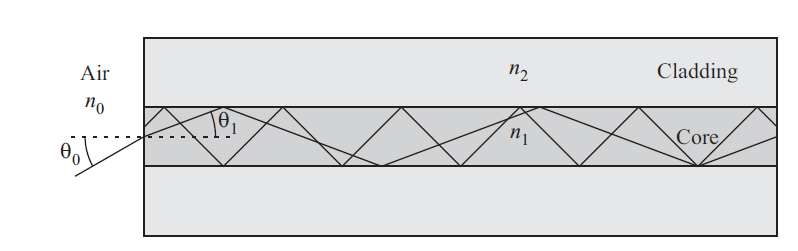
\includegraphics[width=188.4pt]{images/image33.png} 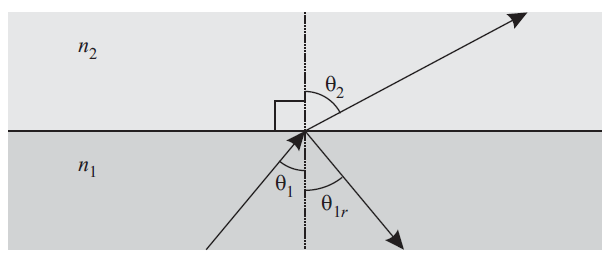
\includegraphics[width=149.9pt]{images/image34.png}
\end{center}
\end{frame}

\begin{frame}[shrink=20,t]{Διασπορά Πολλών Τρόπων (Γεωμετρική Οπτική)}
\begin{itemize}
\item τότε οι ακτίνες ανακλώνται ολικά στις διαχωριστικές επιφάνειες πυρήνα (core) και περιβλήματος (cladding)
\item H \textit{θ}$_{\text{max}}$ ονομάζεται κρίσιμη γωνία (critical angle)
\end{itemize}
\medskip
\begin{itemize}
\item Για την παραπάνω γεωμετρία είναι δυνατόν να δείξουμε ότι αν \textit{θ}$_{\text{0}}$<\textit{θ}$_{\text{max}}$ όπου
\end{itemize}
\begin{center}
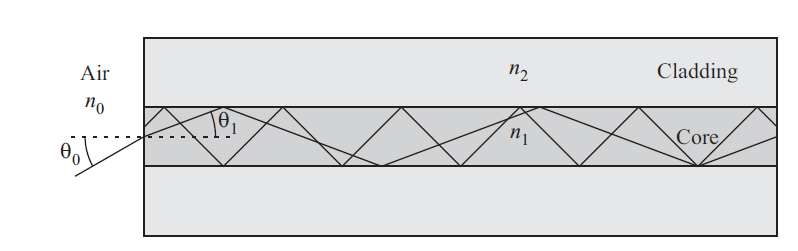
\includegraphics[width=338.3pt]{images/image33.png}
\end{center}
\begin{center}
$\displaystyle \theta_{\max}=\sin^{-1}\frac{\sqrt{n_{1}^{2}-n_{2}^{2}}}{n_{0}}$\\[0.6ex]
\end{center}
\end{frame}

\begin{frame}[shrink=20,t]{Χρονική Διεύρυνση}
\begin{itemize}
\item Η πιο γρήγορη ακτίνα χρειάζεται χρόνο \textit{Τ}$_{\text{\textit{f}}}$=\textit{Ln}$_{\text{1}}$/\textit{c }για να φτάσει στην έξοδο.
\item Η πιο αργή ακτίνα εισέρχεται στην ίνα υπό γωνία \textit{θ}$_{\text{1}}$ (δείτε προηγούμενο σχήμα)
\item Η συνολική απόσταση που πρέπει να καλύψει η αργή ακτίνα είναι \textit{L}\textit{/}sin\textit{θ}$_{\text{1}}$.
\item Από τον νόμο της διάθλασης έχουμε \textit{n}$_{\text{1}}$sin\textit{θ}$_{\text{1}}$=\textit{n}$_{\text{0}}$sin\textit{θ}$_{\text{max}}$ και αν θεωρήσουμε πως \textit{n}$_{\text{0}}$=1 (αέρας) τότε sin\textit{θ}$_{\text{1}}$=1/\textit{n}$_{\text{1}}$.
\item Ό χρόνος επομένως που χρειάζεται η αργή ακτίνα είναι \textit{T}$_{\text{\textit{s}}}$=\textit{Ln}$_{\text{1}}$/\textit{c}\textit{/}\textit{sin}\textit{θ}$_{\text{1}}$\textit{=}\textit{Ln}$_{\text{1}}$$^{\text{\textit{2}}}$\textit{/c/n}$_{\text{2}}$\textit{.}
\item H χρονική διεύρυνση είναι επομένως δ\textit{Τ}=\textit{Τ}$_{\text{\textit{s}}}$\ensuremath{-}\textit{T}$_{\text{\textit{f}}}$=\textit{L}/\textit{cn}$_{\text{1}}$$^{\text{2}}$/\textit{n}$_{\text{2}}$Δ όπου Δ=(\textit{n}$_{\text{1}}$-\textit{n}$_{\text{2}}$)/\textit{n}$_{\text{1}}$.
\item Αν υποθέσουμε ότι ο χρόνος διεύρυνσης δεν πρέπει να γίνει μεγαλύτερος από το ήμισυ της διάρκειας του bit τότε βρίσκουμε ότι το γινόμενο ρυθμού-απόστασης (bit rate-distance product) είναι:
\end{itemize}
\begin{center}
$\displaystyle BL\le\frac{1}{2}\,\frac{n_{2}}{n_{1}^{2}}\,\frac{c}{\Delta}$\\[0.6ex]
\end{center}
\end{frame}

\begin{frame}[shrink=20,t]{Πολύτροπες Ίνες}
\begin{itemize}
\item Χρησιμοποιούνται σε τοπικά δίκτυα (local area networks)
\item Με LEDs πετυχαίνουμε ρυθμούς της τάξης των 600Mb/s
\item Με LASER μπορούμε να πετύχουμε και ρυθμούς της τάξης των Gb/s.
\item EMB = Effective mode bandwidth
\item OFLBW=Overfilled launch bandwidth
\end{itemize}
\begin{center}
\setlength{\unitlength}{0.000044pt}
\begin{picture}(8143875,2381250)
\put(0,0){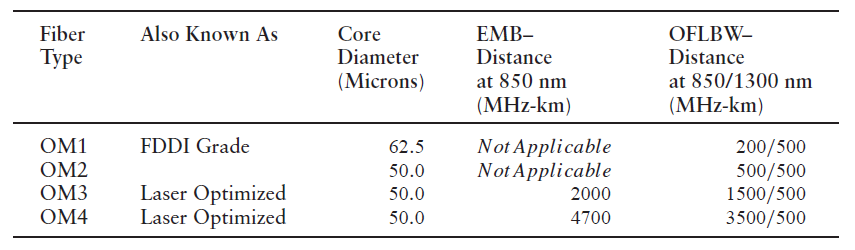
\includegraphics[width=358.2pt]{images/image37.png}}
\put(6935948,2297670){\footnotesize \shortstack{LED}}
\put(4844742,2226232){\footnotesize \shortstack{LASER}}
\end{picture}
\end{center}
\end{frame}

\begin{frame}[shrink=20,t]{Μονότροπες Ίνες}
\begin{itemize}
\item Όσο πιο μικρό είναι το Δ=(\textit{n}$_{\text{1}}$-\textit{n}$_{\text{2}}$)/\textit{n}$_{\text{1}}$ τόσο πιο μικρό είναι το V και επομένως τόσο πιο εύκολο είναι να πετύχουμε μονότροπη λειτουργία.
\item Το γεγονός ότι έχουμε \textit{n}$_{\text{1}}$\ensuremath{\cong}\textit{n}$_{\text{2}}$ σημαίνει πως έχουμε \textit{ασθενή }\textit{κυματοδήγηση}\textit{.} Το κύμα εξασθενεί σχετικά αργά όσο απομακρυνόμαστε από το κέντρο της ίνας
\end{itemize}
\medskip
\begin{itemize}
\item Στην περίπτωση όπου η ακτίνα της ίνας είναι συγκρίσιμη με το μήκος κύματος δεν μπορούμε να χρησιμοποιήσουμε την γεωμετρική προσέγγιση
\item Το πεδίο αναπτύσσεται σε μία σειρά τρόπων και υπό κατάλληλες συνθήκες μπορούμε να έχουμε την ύπαρξη ενός και μόνο τρόπου
\item Η συνθήκη για μονότροπη διάδοση είναι:
\end{itemize}
\begin{center}
$\displaystyle V=\frac{2\pi a}{\lambda}\sqrt{n_{1}^{2}-n_{2}^{2}}<2.405$\\[0.6ex]
\end{center}
\end{frame}

\begin{frame}[shrink=20,t]{Ενεργός δείκτης διάθλασης}
\begin{itemize}
\item Εξαιτίας της αλλαγής του δείκτη διάθλασης από \textit{n}$_{\text{1}}$ σε \textit{n}$_{\text{2}}$, το κύμα δεν διαδίδεται στον ελεύθερο χώρο αλλά σε ένα ανομοιογενές μέσο διάδοσης
\item Τα χαρακτηριστικά του μέσου διάδοσης (γεωμετρία + προφίλ δείκτη διάθλασης) αποτυπώνονται στον τρόπο διάδοσης του οποίου τα χαρακτηριστικά διαφέρουν από αυτά του ελεύθερου χώρου.
\item Σε ένα ομοιογενές μέσο με δ.δ. \textit{n}$_{\text{1}}$ το κύμα έχει σταθερά διάδοσης ίση με \textit{β}=(2π/λ)\textit{n}$_{\text{1}}$. Αυτό σημαίνει πως η φάση του κύματος όταν αυτό διαδίδεται στη διεύθυνση του άξονα \textbf{z} είναι exp(\textit{j}\textit{β}\textit{z}).
\item Στην περίπτωση της ίνας αντί για \textit{β}=(2π/λ)\textit{n}$_{\text{1}}$ έχουμε \textit{ β}=(2π/λ)\textit{n}$_{\text{\textit{eff}}}$\textit{ }όπου το \textit{n}$_{\text{\textit{eff}}}$ είναι ο ενεργός δείκτης διάθλασης.
\item οι τιμές του \textit{n}$_{\text{\textit{eff}}}$ είναι \textit{n}$_{\text{2}}$\ensuremath{\le}\textit{n}$_{\text{eff}}$\ensuremath{\le}\textit{n}$_{\text{1}}$. Για 1.5\ensuremath{\le}\textit{V}\ensuremath{\le}2.5, καθορίζονται προσεγγιστικά από την εξίσωση:
\end{itemize}
\begin{center}
$\displaystyle \frac{n_{\mathrm{eff}}^{2}-n_{2}^{2}}{n_{1}^{2}-n_{2}^{2}}\approx\left(1.1428-\frac{0.996}{V}\right)^{2}$\\[0.6ex]
\end{center}
\end{frame}

\begin{frame}[shrink=20,t]{Εξισώσεις Maxwell (*)}
\begin{itemize}
\item Οι εξισώσεις Maxwell διέπουν την διάδοση των κυμάτων εντός της οπτικής ίνας
\item Οι προηγούμενες σχέσεις προκύπτουν από τις εξισώσεις Maxwell που σχετίζουν το ηλεκτρικό πεδίο \textbf{E }και το μαγνητικό πεδίο \textbf{H} μεταξύ τους.
\item Το \textit{ε} είναι η διηλεκτρική σταθερά του μέσου και σχετίζεται με το δείκτη διάθλασης, \textit{ε}=\textit{ε}$_{\text{0}}$\textit{n}$^{\text{2}}$
\item \textit{ε}$_{\text{0}}$ και \textit{μ}$_{\text{0}}$ είναι η ηλεκτρική και μαγνητική διαπερατότητα του κενού.
\end{itemize}
\begin{center}
$\displaystyle \nabla\times\mathbf{E}=-\mu_{0}\frac{\partial\mathbf{H}}{\partial t}$ $\displaystyle \nabla\times\mathbf{H}=\epsilon\frac{\partial\mathbf{E}}{\partial t}$\\[0.6ex]
$\displaystyle \nabla\cdot(\epsilon\mathbf{E})=0$ $\displaystyle \nabla\cdot\mathbf{H}=0$\\[0.6ex]
\end{center}
\end{frame}

\begin{frame}[shrink=20,t]{Πεδίο των Συχνοτήτων}
\begin{itemize}
\item Κάθε σήμα \textit{x}(\textit{t}) στο πεδίο του χρόνου μπορεί να αναπαρασταθεί  στο πεδίο των συχνοτήτων μέσω του μετασχηματισμού Fourier \textit{X}(\textit{ω}).
\end{itemize}
\medskip
\begin{itemize}
\item Παρόμοιες σχέσεις ισχύουν και τις συνιστώσες του ηλεκτρικού και του μαγνητικού πεδίου:
\end{itemize}
\begin{center}
$\displaystyle X(\omega)=\int\limits_{-\infty}^{+\infty}dt\,x(t)\,e^{-j\omega t}$ $\displaystyle x(t)=\int\limits_{-\infty}^{+\infty}d\omega\,X(\omega)\,e^{j\omega t}$\\[0.6ex]
$\displaystyle \tilde{E}_{x}(\mathbf{r},\omega)=\int\limits_{-\infty}^{+\infty}dt\,E_{x}(\mathbf{r},t)\,e^{-j\omega t}$ $\displaystyle E_{x}(\mathbf{r},t)=\int\limits_{-\infty}^{+\infty}d\omega\,\tilde{E}_{x}(\mathbf{r},\omega)\,e^{j\omega t}$\\[0.6ex]
\end{center}
\end{frame}

\begin{frame}[t]{Εξισώσεις Maxwell στο Συχνοτικό Πεδίο (*)}
\begin{center}
$\displaystyle \nabla\times\tilde{\mathbf{E}}=-j\omega\mu_{0}\tilde{\mathbf{H}}$\\[0.6ex]
$\displaystyle \nabla\times\tilde{\mathbf{H}}=j\omega\epsilon\tilde{\mathbf{E}}$\\[0.6ex]
$\displaystyle \nabla\cdot\tilde{\mathbf{E}}=0$\\[0.6ex]
$\displaystyle \nabla\cdot\tilde{\mathbf{H}}=0$\\[0.6ex]
$\displaystyle \frac{\partial}{\partial t}e^{j\omega t}=j\omega\,e^{j\omega t}$\\[0.6ex]
\end{center}
\end{frame}

\begin{frame}[shrink=20,t]{Ηλεκτρομαγνητική Ανάλυση Οπτικών Ινών (*)}
\begin{itemize}
\item Στην περίπτωση της οπτικής ίνας, χρησιμοποιούμε το γεγονός ότι η διηλεκτρική σταθερά και ο δείκτης διάθλασης δεν εξαρτώνται από τη διεύθυνση διάδοσης (z)
\item Δηλαδή \textit{ε}=\textit{ε}(\textit{x},\textit{y},\textit{z})=\textit{ε}(\textit{x},\textit{y})
\end{itemize}
\begin{center}
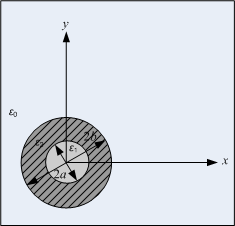
\includegraphics[width=119.0pt]{images/image53.png} 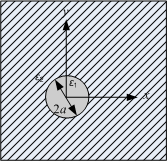
\includegraphics[width=118.6pt]{images/image54.png} 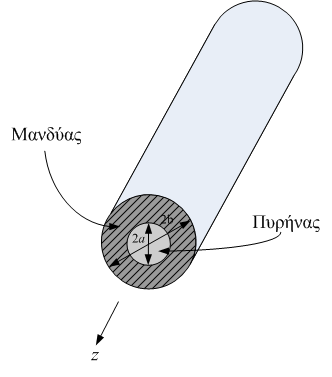
\includegraphics[width=100.8pt]{images/image55.png}
\end{center}
\end{frame}

\begin{frame}[shrink=20,t]{Ηλεκτρομαγνητική Ανάλυση Οπτικών Ινών (*)}
\begin{center}
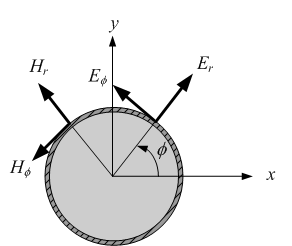
\includegraphics[width=231.0pt]{images/image61.png}
\end{center}
\begin{center}
$\displaystyle \mathbf{H}_{T}=-\frac{j\omega\epsilon}{p^{2}}\,\hat{\mathbf{z}}\times\nabla_{T}E_{z}-\frac{j\beta}{p^{2}}\nabla_{T}H_{z}$\\[0.6ex]
$\displaystyle \mathbf{E}_{T}=-\frac{j\beta}{p^{2}}\nabla_{T}E_{z}+\frac{j\omega\mu_{0}}{p^{2}}\,\hat{\mathbf{z}}\times\nabla_{T}H_{z}$\\[0.6ex]
$\displaystyle \nabla_{T}^{2}E_{z}+p^{2}E_{z}=\frac{1}{\rho}\frac{\partial}{\partial\rho}\left(\rho\frac{\partial E_{z}}{\partial\rho}\right)+\frac{1}{\rho^{2}}\frac{\partial^{2}E_{z}}{\partial\phi^{2}}+p^{2}E_{z}=0$\\[0.6ex]
$\displaystyle \nabla_{T}^{2}H_{z}+p^{2}H_{z}=\frac{1}{\rho}\frac{\partial}{\partial\rho}\left(\rho\frac{\partial H_{z}}{\partial\rho}\right)+\frac{1}{\rho^{2}}\frac{\partial^{2}H_{z}}{\partial\phi^{2}}+p^{2}H_{z}=0$\\[0.6ex]
$\displaystyle p=\sqrt{\omega^{2}\mu\epsilon_{1}-\beta^{2}}$\\[0.6ex]
\end{center}
\end{frame}

\begin{frame}[shrink=20,t]{Ηλεκτρομαγνητική Ανάλυση Οπτικών Ινών (*)}
\begin{itemize}
\item Στη διαχωριστική επιφάνεια θα πρέπει να εγγυηθούμε την συνέχεια των συνιστωσών του ηλεκτρικού και του μαγνητικού πεδίου
\end{itemize}
\medskip
\begin{itemize}
\item Εντός του πυρήνα της ίνας (\textit{ρ}<\textit{a})
\end{itemize}
\medskip
\begin{itemize}
\item Στο μανδύα της ίνας (\textit{ρ}>\textit{a})
\end{itemize}
\begin{center}
$\displaystyle E_{z}=\frac{J_{m}(p\rho)}{J_{m}(pa)}\bigl(A_{1}\cos(m\phi)+B_{1}\sin(m\phi)\bigr)$\\[0.6ex]
$\displaystyle E_{z}=\frac{K_{m}(q\rho)}{K_{m}(qa)}\bigl(A_{2}\cos(m\phi)+B_{2}\sin(m\phi)\bigr)$\\[0.6ex]
\end{center}
\end{frame}

\begin{frame}[shrink=20,t]{Τρόποι Διάδοσης σε μία Οπτική Ίνα (*)}
\begin{itemize}
\item Η παραπάνω θεωρία οδηγεί στις χαρακτηριστικές εξισώσεις για τους τρόπους της ίνας
\end{itemize}
\medskip
\begin{itemize}
\item Τρόποι ΗΕ
\end{itemize}
\medskip
\begin{itemize}
\item Τρόποι ΕΗ
\end{itemize}
\medskip
\begin{itemize}
\item Τρόποι TE+TM
\end{itemize}
\begin{center}
$\displaystyle \frac{1}{pa}\frac{J^{\prime}_{m}(pa)}{J_{m}(pa)}+\frac{1}{qa}\frac{K^{\prime}_{m}(qa)}{K_{m}(qa)}\cong +m\left\{\frac{1}{p^{2}a^{2}}+\frac{1}{q^{2}a^{2}}\right\}$\\[0.6ex]
$\displaystyle \frac{1}{pa}\frac{J^{\prime}_{m}(pa)}{J_{m}(pa)}+\frac{1}{qa}\frac{K^{\prime}_{m}(qa)}{K_{m}(qa)}\cong -m\left\{\frac{1}{p^{2}a^{2}}+\frac{1}{q^{2}a^{2}}\right\}$\\[0.6ex]
$\displaystyle \frac{1}{pa}\frac{J^{\prime}_{0}(pa)}{J_{0}(pa)}+\frac{1}{qa}\frac{K^{\prime}_{0}(qa)}{K_{0}(qa)}\cong 0$ $\displaystyle p^{2}a^{2}+q^{2}a^{2}=V^{2}$\\[0.6ex]
\end{center}
\end{frame}

\begin{frame}[t]{Τρόποι Διάδοσης σε μία Οπτική Ίνα (*)}
\begin{itemize}
\item Όταν \textit{n}$_{\text{1}}$\ensuremath{>}\textit{n}$_{\text{2}}$ τότε το μέσο είναι σχεδόν ομογενές και περιμένουμε οι τρόποι να είναι  εγκάρσιοι
\item \textit{E}$_{\text{\textit{z}}}$,\textit{H}$_{\text{\textit{z}}}$\ensuremath{>}0
\end{itemize}
\end{frame}

\begin{frame}[shrink=10,t]{Τρόποι Διάδοσης σε μία Οπτική Ίνα (*)}
\begin{center}
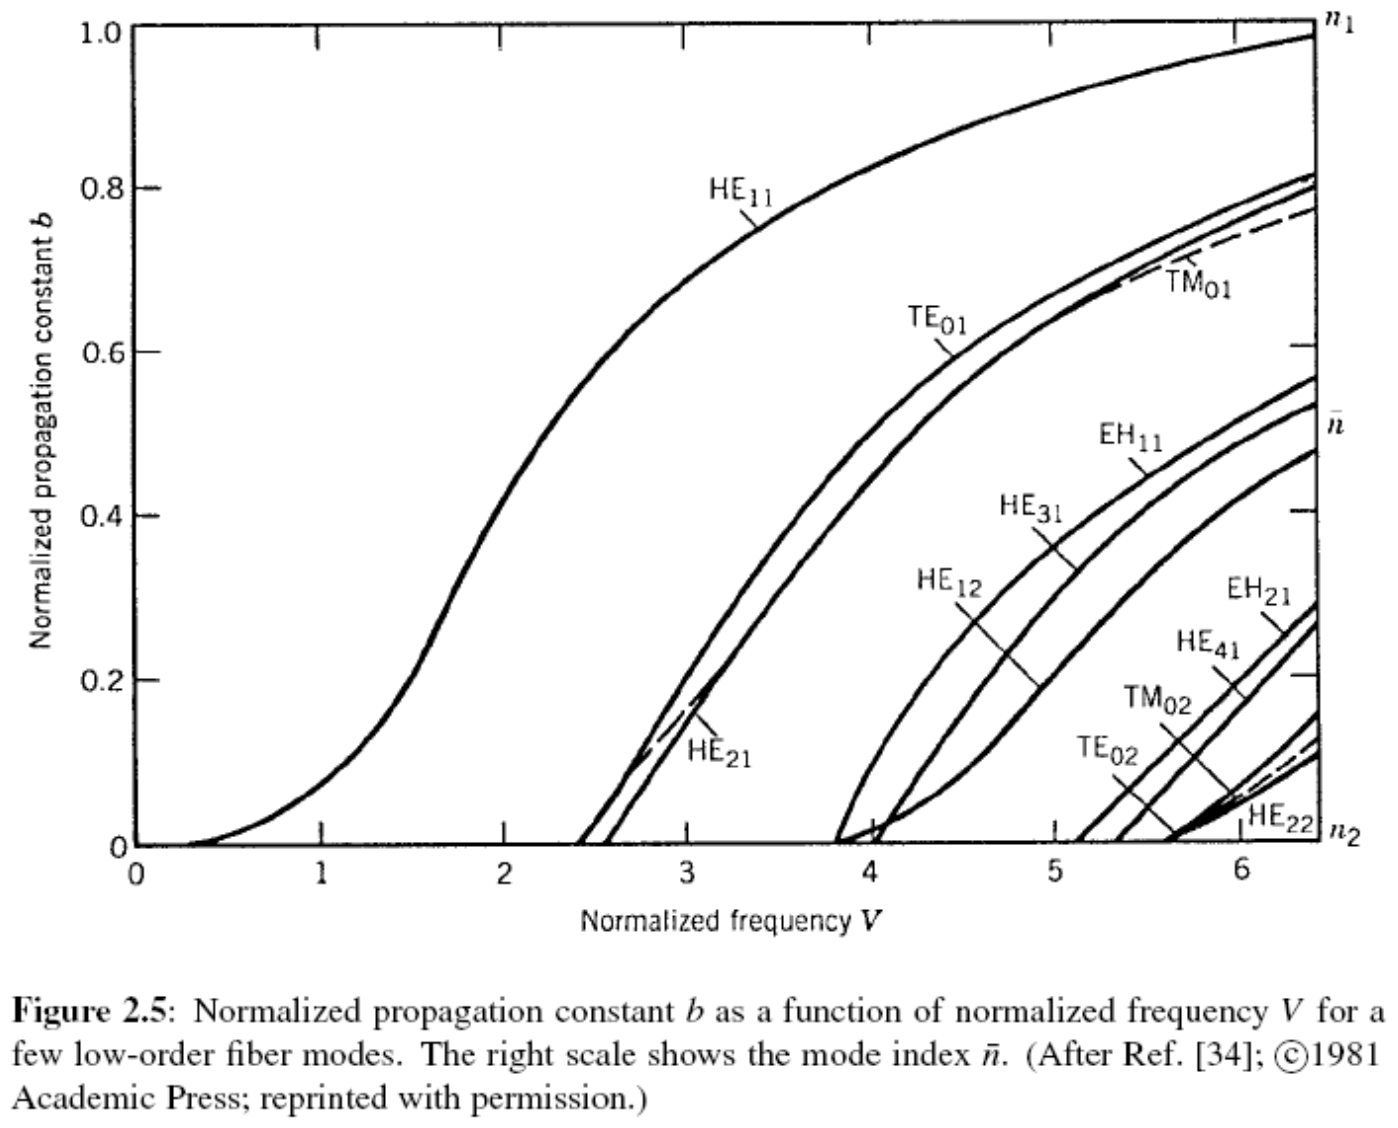
\includegraphics[height=0.62\textheight]{images/image69.png}\\[1ex]
Μονότροπη Ίνα: $\displaystyle V<2.405$
\end{center}
\end{frame}

\begin{frame}[shrink=20,t]{Χρωματική Διασπορά}
\begin{itemize}
\item Ας υποθέσουμε πως ένα σήμα \textit{x}(\textit{t}) εισέρχεται σε μία οπτική ίνα.
\item Κάθε συνιστώσα του φάσματος \textit{Χ}(\textit{ω}) του \textit{x}(\textit{t}) μπορούμε να θεωρήσουμε ότι διαδίδεται ανεξάρτητα.
\item Επομένως (αν αγνοήσουμε την εξασθένιση) η συνιστώσα εμφανίζεται στην έξοδο με ολισθημένη φάση \textit{Χ}(\textit{ω})\textit{e}$^{\text{\textit{j}}}$$^{\text{\textit{β}}}$$^{\text{\textit{z}}}$
\item Στην περίπτωση του ελεύθερου χώρου θα είχαμε \textit{β}(\textit{ω})=2π/\textit{λ}=\textit{ω}/\textit{c }και επομένως το φάσμα εξόδου θα είναι  \textit{Υ}(\textit{ω})=\textit{Χ}(\textit{ω})\textit{e}$^{\text{\textit{j}}}$$^{\text{(}}$$^{\text{\textit{ω}}}$$^{\text{/}}$$^{\text{\textit{c}}}$$^{\text{)}}$$^{\text{\textit{z}}}$.
\item Το αντίστοιχο σήμα στο πεδίο του χρόνου υπολογίζεται ως εξής:
\end{itemize}
\medskip
\begin{itemize}
\item Επομένως στην περίπτωση όπου η οπτική ίνα είχε τα ίδια χαρακτηριστικά με τον ελεύθερο χώρο, το σήμα θα παρουσιαζότανε με καθυστέρηση \textit{z}/\textit{c}
\item Αυτό είναι σύμφωνο με το γεγονός πως το φως διαδίδεται με ταχύτητα ίση με \textit{c} στον ελεύθερο χώρο…
\end{itemize}
\begin{center}
$\displaystyle y(t)=\int\limits_{-\infty}^{+\infty}Y(\omega)e^{-j\omega t}d\omega=\int\limits_{-\infty}^{+\infty}X(\omega)e^{j(\omega/c)z-j\omega t}d\omega=x\left(t-\frac{z}{c}\right)$\\[0.6ex]
\end{center}
\end{frame}

\begin{frame}[shrink=20,t]{Χρωματική Διασπορά}
\begin{itemize}
\item Στην περίπτωση της οπτικής ίνας, δεν μπορούμε να υποθέσουμε ότι \textit{β}(\textit{ω})=\textit{ω}/\textit{c}. Η σχέση \textit{β} και \textit{ω} είναι μη γραμμική.
\item Μπορούμε να χρησιμοποιήσουμε το ανάπτυγμα του Taylor ώστε να γράψουμε το β ως πολυώνυμο του \textit{ω} κοντά στην κεντρική συχνότητα του σήματος \textit{ω}$_{\text{0}}$, \textit{β}(\textit{ω})\ensuremath{-}\textit{β}(\textit{ω}$_{\text{0}}$)=\textit{β}$_{\text{1}}$(ω$_{\text{0}}$)Δ\textit{ω}+\textit{β}$_{\text{2}}$(ω$_{\text{0}}$)Δ\textit{ω}$^{\text{2}}$/2+\textit{β}$_{\text{3}}$(\textit{ω}$_{\text{0}}$)Δ\textit{ω}$^{\text{3}}$/6+…, όπου Δ\textit{ω}=\textit{ω}-\textit{ω}$_{\text{0}}$
\item Οι συντελεστές \textit{β}$_{\text{\textit{i}}}$ καθορίζονται από τις παραγώγους της \textit{β}(\textit{ω}) στο \textit{ω}=\textit{ω}$_{\text{0}}$, \textit{β}$_{\text{\textit{i}}}$=d$^{\text{\textit{i}}}$\textit{β}(\textit{ω}$_{\text{0}}$)/d\textit{ω}$^{\text{\textit{i}}}$
\item Το \textit{β}$_{\text{1}}$ είναι το αντίστροφο της ταχύτητας ομάδας \textit{v}$_{\text{\textit{g}}}$, \textit{β}$_{\text{1}}$=d\textit{β}/d\textit{ω}=(d\textit{ω}/d\textit{β})$^{\text{-1}}$=1/\textit{v}$_{\text{\textit{g}}}$.
\item Η παράμετρος \textit{β}$_{\text{2}}$ ονομάζεται συντελεστής διασποράς ταχύτητας ομάδας (Group Velocity Dispersion-GVD). Μετριέται σε ps$^{\text{2}}$/Km.
\item Ο συντελεστής \textit{β}$_{\text{3}}$ ονομάζεται συντελεστής διασποράς ανώτερης τάξης.
\end{itemize}
\end{frame}

\begin{frame}[shrink=20,t]{Διεύρυνση Παλμών εξαιτίας GVD}
\begin{itemize}
\item To μήκος \textit{L}$_{\text{\textit{D}}}$ είναι το χαρακτηριστικό μήκος της GVD το οποίο δίνεται από την σχέση \textit{L}$_{\text{\textit{D}}}$=\textit{T}$_{\text{0}}$$^{\text{2}}$/|\textit{β}$_{\text{2}}$|
\item Στην παραπάνω σχέση, \textit{T}$_{\text{\textit{z}}}$ είναι το εύρος του παλμού σε απόσταση \textit{z}, \textit{T}$_{\text{0}}$ το αρχικό εύρος του παλμού, \textit{z} η απόσταση που έχει διαδοθεί το σήμα.
\end{itemize}
\medskip
\begin{itemize}
\item Χρησιμοποιώντας το μετασχηματισμό Fourier μπορούμε να υπολογίσουμε την διεύρυνση των παλμών εξαιτίας του \textit{β}$_{\text{2}}$ (θεωρώντας ότι \textit{β}$_{\text{3}}$=0)
\end{itemize}
\begin{center}
$\displaystyle \frac{T_{z}}{T_{0}}=\sqrt{1+\left(\frac{\beta_{2}z}{T_{0}^{2}}\right)^{2}}=\sqrt{1+\left(\frac{z}{L_{D}}\right)^{2}}$\\[0.6ex]
\end{center}
\end{frame}

\begin{frame}[shrink=20,t]{Συντελεστής διασποράς D}
\begin{itemize}
\item Συνήθως αντί του β2 χρησιμοποιούμε την παράμετρο \textit{D}=-(2π\textit{c}/\textit{λ}$^{\text{2}}$)\textit{β}$_{\text{2}}$.
\item Στις οπτικές ίνες έχουμε \textit{D}=\textit{D}$_{\text{M}}$+\textit{D}$_{\text{W}}$ όπου το \textit{D}$_{\text{M}}$ οφείλεται στη διασπορά του μέσου ενώ το \textit{D}$_{\text{W}}$ οφείλεται στη κυματοδήγηση.
\end{itemize}
\medskip
\begin{itemize}
\item Συντελεστής διασποράς D μίας οπτικής ίνας
\end{itemize}
\begin{center}
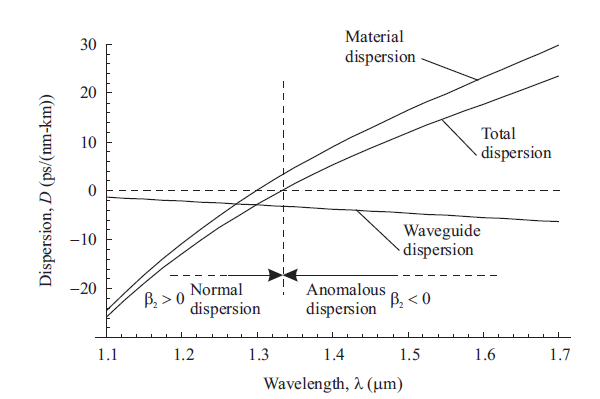
\includegraphics[width=225.6pt]{images/image73.png}
\end{center}
\end{frame}

\begin{frame}[shrink=20,t]{Έλεγχος της GVD}
\begin{itemize}
\item Δεν μπορούμε να αλλάξουμε εύκολα τις τιμές του DM αλλά ωστόσο μπορούμε να επέμβουμε στην DW
\item Αυτό το κάνουμε μεταβάλλοντας το προφίλ του δείκτη διάθλασης. Με τον τρόπο αυτό μπορούμε να έχουμε διαφορετική συμπεριφορά ως προς την διασπορά στο λ=1.55μm
\end{itemize}
\begin{center}
\setlength{\unitlength}{0.000057pt}
\begin{picture}(6248400,1866900)
\put(0,0){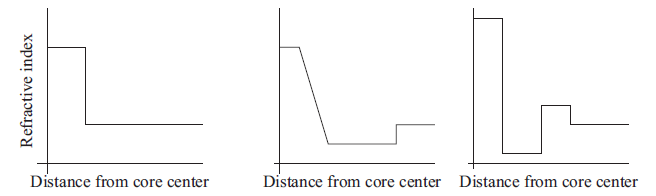
\includegraphics[width=358.2pt]{images/image74.png}}
\put(863905,1783320){\footnotesize \shortstack{Standard}}
\put(3324360,1783320){\footnotesize \shortstack{DSF}}
\put(4643562,1649197){\footnotesize \shortstack{Dispersion Compensating}}
\end{picture}
\end{center}
\end{frame}

\begin{frame}[shrink=10,t]{Παραδείγματα}
\begin{center}
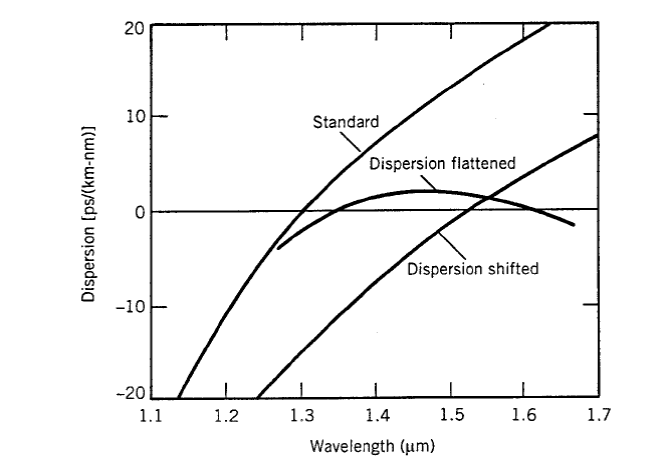
\includegraphics[width=276.5pt]{images/image75.png}
\end{center}
\end{frame}

\begin{frame}[shrink=10,t]{Φαινόμενα Πόλωσης (Polarization)}
\begin{itemize}
\item H προηγούμενη ανάλυση τρόπων έδειξε πως σε μία ιδανική (τελείως κυκλικής διατομής) μονότροπη οπτική  ίνα υπάρχει μόνο ένας  τρόπος διάδοσης (ΗΕ11)
\item Στην πράξη όμως οι οπτικές ίνες δεν είναι τέλεια κυκλικές. Αυτό έχει ως αποτέλεσμα ο ΗΕ11 να χωρίζεται σε δύο τρόπους των οποίων το ηλεκτρικό πεδίο είναι πολωμένο σε διαφορετικό άξονα.
\item Επίσης επειδή η διατομή μεταβάλλεται κατά μήκος της ίνας, οι άξονες αυτοί δεν είναι σταθεροί αλλά περιστρέφονται τυχαία!
\item Οι δύο τρόποι διάδοσης έχουν ελαφρώς διαφορετικής σταθερά διάδοσης και επομένως έχουμε ένα είδος διασποράς δύο τρόπων.
\item Σε κάθε περίπτωση μιλάμε για διασπορά τρόπου πόλωσης (polarization mode dispersion – PMD).
\end{itemize}
\end{frame}

\begin{frame}[shrink=20,t]{Φαινόμενα Πόλωσης (Polarization)}
\begin{itemize}
\item Η διασπορά πόλωσης χαρακτηρίζεται από το συντελεστή differential group delay (DGD) \textit{D}$_{\text{\textit{p}}}$
\item Η διεύρυνση του παλμού δίνεται από τη σχέση Δ\textit{τ}=\textit{D}$_{\text{\textit{p}}}$\textit{L}$^{\text{1/2}}$.
\end{itemize}
\begin{center}
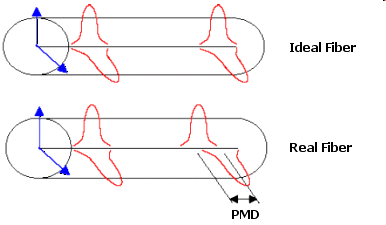
\includegraphics[width=257.3pt]{images/image76.png}
\end{center}
\end{frame}

\begin{frame}[shrink=20,t]{Μη γραμμικά φαινόμενα}
\begin{itemize}
\item Η ίνα είναι ένα μη γραμμικό μέσο: η συμπεριφορά της εξαρτάται από την ισχύ του σήματος.
\item Για ισχύ μερικών mW και ρυθμούς της τάξης των 2.5Gb/s τα μη γραμμικά φαινόμενα μπορούν να αγνοηθούν.
\item Για ρυθμούς τις τάξης των 10Gb/s και υψηλότερη ισχύ η επίδραση των μη γραμμικών φαινομένων γίνεται πιο σημαντική.
\item Στην περίπτωση WDM η ίνα μεταφέρει πολλά κανάλια και επομένως η συνολική ισχύς είναι ακόμα μεγαλύτερη.
\item Υπάρχουν δύο είδη μη γραμμικών φαινομένων:
\begin{itemize}
\item Αλληλεπίδραση οπτικών κυμάτων και φωνονίων (μοριακές δονήσεις) στο μέσο διάδοσης: Εξαναγκασμένη σκέδαση Raman και Brillouin.
\item Μη γραμμική εξάρτηση του δείκτη διάθλασης του μέσου από την οπτική ισχύ: Self Phase Modulation (SPM), Cross Phase Modulation (XPM) και μίξη τεσσάρων κυμάτων (FWM).
\end{itemize}
\end{itemize}
\end{frame}

\begin{frame}[shrink=20,t]{Μεγέθη που επηρεάζουν την ένταση των φαινομένων}
\begin{itemize}
\item Υπάρχουν δύο μεγέθη που καθορίζουν την ένταση των μη γραμμικών φαινομένων.
\begin{itemize}
\item Ενεργό μήκος διάδοσης \textit{L}$_{\text{\textit{e}}}$: Το μήκος το οποίο πολλαπλασιαζόμενο με την ισχύ κορυφής εισόδου μας δίνει το ολοκλήρωμα της ισχύος κατά μήκος της διάδοσης. Μεγάλο \textit{L}$_{\text{\textit{e}}}$ σημαίνει πως το σήμα δεν εξασθενεί γρήγορα λόγω απωλειών άρα τα μη γραμμικά φαινόμενα θα είναι ενισχυμένα.
\item Ενεργή επιφάνεια \textit{Α}$_{\text{\textit{e}}}$. Υπολογίζεται από το ολοκλήρωμα της πυκνότητας ισχύος (ένταση) του κύματος. Μετράει πόσο συγκεντρωμένη είναι η πυκνότητα ισχύος πάνω στην διατομή της ίνας. Μικρή \textit{A}$_{\text{\textit{e}}}$ σημαίνει μεγάλη ένταση και επομένως ισχυρότερα μη γραμμικά φαινόμενα.
\end{itemize}
\end{itemize}
\begin{center}
$\displaystyle A_{e}=\frac{\left(\int\limits_{S}dx\,dy\,|F(x,y)|^{2}\right)^{2}}{\int\limits_{S}dx\,dy\,|F(x,y)|^{4}}$\\[0.6ex]
$\displaystyle P_{0}L_{e}=\int\limits_{0}^{z}\underbrace{P_{0}e^{-az}}_{P(z)}dz\;\rightarrow\;L_{e}=\frac{1-e^{-az}}{a}$\\[0.6ex]
\end{center}
\end{frame}

\begin{frame}[shrink=10,t]{Εξαναγκασμένη Σκέδαση Brillouin}
\begin{itemize}
\item Στην σκέδαση Brillouin:
\begin{itemize}
\item Έχουμε οπισθοσκέδαση (το κύμα που σκεδάζεται κινείται προς τα πίσω).
\item Είναι φαινόμενο στενού εύρους ζώνης (\ensuremath{\le}100ΜΗz). Επομένως ένα κανάλι δεν επηρεάζει άλλα κανάλια που απέχουν 50-100GHz.
\item Προκαλείται όμως παραμόρφωση στο ίδιο το κανάλι.
\item Πρέπει να προστατέψουμε τον πομπό από την οπισθοσκέδαση με χρήση απομονωτή (isolator).
\item To φαινόμενο εξαρτάται από την τιμή του κέρδους συντελεστή Brillouin \textit{g}$_{\text{B}}$\ensuremath{\cong}4\ensuremath{\times}10$^{-11}$m/W.
\end{itemize}
\end{itemize}
\end{frame}

\begin{frame}[shrink=20,t]{Εξαναγκασμένη Σκέδαση Brillouin}
\begin{itemize}
\item \textit{Ι}$_{\text{\textit{s}}}$ και \textit{I}$_{\text{\textit{p}}}$ είναι οι εντάσεις του κύματος οπισθοσκέδασης και του αρχικού κύματος.
\item \textit{Ι}$_{\text{\textit{s}}}$=\textit{P}$_{\text{\textit{s}}}$/\textit{A}$_{\text{\textit{e}}}$ και \textit{Ι}$_{\text{\textit{p}}}$=\textit{P}$_{\text{\textit{p}}}$/\textit{A}$_{\text{\textit{e}}}$.
\item Θεωρώντας πως η ισχύς του αρχικού κύματος είναι πολύ μεγαλύτερη από την ισχύ του οπισθοσκεδαζόμενου κύματος \textit{P}$_{\text{\textit{s}}}$ μπορούμε να καταλήξουμε σε μία σχέση για την \textit{P}$_{\text{\textit{s}}}$ στην είσοδο \textit{z}=0.
\end{itemize}
\medskip
\begin{itemize}
\item \ensuremath{\cong}0
\end{itemize}
\begin{center}
$\displaystyle \frac{dI_{s}}{dz}=-g_{B}I_{s}I_{p}+aI_{s}$ $\displaystyle A_{e}=\frac{\left(\int\limits_{S}dA\,\mathrm{Re}\left(\mathbf{E}\times\mathbf{H}^{*}\right)\right)^{2}}{\int\limits_{S}dA\,\left|\mathrm{Re}\left(\mathbf{E}\times\mathbf{H}^{*}\right)\right|^{2}}$\\[0.6ex]
$\displaystyle P_{s}(0)=P_{s}(L)\,e^{-aL}\exp\left(\frac{g_{B}P_{p}(0)L_{e}}{A_{e}}\right)$\\[0.6ex]
$\displaystyle \frac{dI_{p}}{dz}=-g_{B}I_{s}I_{p}-aI_{p}$\\[0.6ex]
\end{center}
\end{frame}

\begin{frame}[shrink=10,t]{Εξαναγκασμένη Σκέδαση Raman}
\begin{center}
\setlength{\unitlength}{0.000056pt}
\begin{picture}(4714875,3228975)
\put(0,0){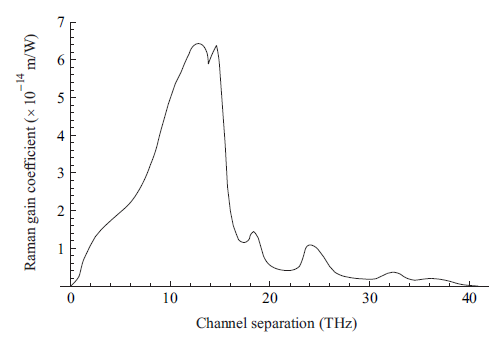
\includegraphics[width=265.8pt]{images/image83.png}}
\end{picture}
\end{center}
\centering\footnotesize Πρόκειται για φαινόμενο ευρείας ζώνης (15THz) Μέσω της σκέδασης Raman μεταφέρεται ισχύς από τα κανάλια σε μικρότερο μήκος κύματος σε κανάλια με μεγαλύτερο μήκος κύματος.\par
\end{frame}

\begin{frame}[shrink=20,t]{Φαινόμενο Kerr}
\begin{itemize}
\item Τα υπόλοιπα μη γραμμικά φαινόμενα πηγάζουν από το γεγονός ότι ο δείκτης \textit{n}(\textit{E}) διάθλασης του μέσω εξαρτάται από την ένταση του πεδίου (Φαινόμενο Kerr)
\item \textit{n}(\textit{E})=\textit{n}$_{\text{0}}$+\textit{n}$_{\text{2}}$\textit{I} όπου \textit{n}$_{\text{0}}$ είναι ο γραμμικός δείκτης διάθλασης και \textit{n}$_{\text{2}}$ είναι ο μη γραμμικός συντελεστής
\item Ο συντελεστής \textit{n}$_{\text{2}}$ μετριέται σε μm$^{\text{2}}$/W και στην περίπτωση μίας SiO$_{\text{2}}$ ίνας είναι ίσος με 2.2$^{-3}$.4\ensuremath{\times}10$^{\text{\ensuremath{-}8}}$μm$^{\text{2}}$/W.
\item H ένταση \textit{Ι} σχετίζεται με το πεδίο \textit{E} βάσης της σχέσης \textit{Ι}=\ensuremath{\tfrac{1}{2}}\textit{c}\textit{ε}$_{\text{0}}$\textit{n}$_{\text{0}}$|\textit{Ε}|$^{\text{2}}$
\item H μη γραμμικότητα θεωρείται στιγμιαία (χωρίς μνήμη)
\item Μη γραμμικός δείκτης διάθλασης σημαίνει πως ένα σήμα υπόκειται σε διαφορά φάσης ανάλογη της έντασης του πεδίου.
\item Ας θεωρήσουμε την διάδοση του σήματος σε ένα πολύ μικρό κομμάτι ίνας μήκους Δz.
\item H κυματομορφή στο σημείο \textit{z} θα είναι \textit{x}(\textit{t}), ενώ στο σημείο \textit{z}+Δ\textit{z} θα είναι \textit{y}(\textit{t})=\textit{x}(\textit{t})exp(\textit{j}γ|\textit{x}(\textit{t})|$^{\text{2}}$Δ\textit{z})\ensuremath{\cong}\textit{x}(t)+\textit{j}γΔ\textit{z}|\textit{x}(\textit{t})|$^{\text{2}}$\textit{x}(\textit{t})
\item Εφόσον \textit{y}(\textit{t})=\textit{x}(\textit{t})exp(\textit{j}γ|\textit{x}(\textit{t})|$^{\text{2}}$Δ\textit{z}) συνεπάγεται ότι |\textit{x}(\textit{t})|=|\textit{y}(\textit{t})|.
\item H παραπάνω εξίσωση υποδεικνύει πως το φαινόμενο Kerr είναι μία μη-γραμμικότητα τρίτης τάξεως.
\item Το γ είναι ο συντελεστής αυτοδιαμόρφωσης φάσης (SPM).
\end{itemize}
\end{frame}

\begin{frame}[shrink=20,t]{Αυτοδιαμόρφωση Φάσης (Self Phase Modulation –SPM)}
\begin{itemize}
\item Παρουσία απωλειών, \textit{y}(\textit{t})=\textit{x}(\textit{t})exp(-\ensuremath{\tfrac{1}{2}}\textit{az}+\textit{j}γ|\textit{x}(\textit{t})|$^{\text{2}}$Δ\textit{z}) συνεπάγεται ότι |\textit{x}(\textit{t})|=|\textit{y}(\textit{t})|exp(-\ensuremath{\tfrac{1}{2}}\textit{az}).
\item Θεωρούμε έναν Gauss παλμό στην είσοδο μίας ίνας \textit{x}(\textit{t})=\textit{P}$_{\text{0}}$exp(-\textit{t}$^{\text{2}}$/2/\textit{t}$_{\text{0}}$$^{\text{2}}$)
\item Επίσης υποθέτουμε πως η διασπορά δεν παίζει ρόλο κατά την διάδοση του σήματος.
\item Χωρίζουμε την ίνα σε μικρά κομμάτια Δz. Σε κάθε κομμάτι ολισθαίνει η φάση κατά  γ|\textit{x}$_{\text{\textit{n}}}$(\textit{t})|$^{\text{2}}$Δ\textit{z=}\textit{γ}exp(-\textit{az}$_{\text{\textit{n}}}$/2)|\textit{x}(\textit{t})|$^{\text{2}}$ όπου \textit{x}$_{\text{\textit{n}}}$(\textit{t}) είναι το σήμα στην είσοδο του nοστού κομματιού που βρίσκεται στο \textit{z}=\textit{z}$_{\text{\textit{n}}}$
\item Η συνολική μεταβολή της φάσης θα είναι \textit{γ}\ensuremath{\sum}exp(\ensuremath{-}\textit{az}$_{\text{\textit{n}}}$\textit{/2})|\textit{x}(\textit{t})|$^{\text{2}}$Δ\textit{z}=\textit{γ}|\textit{x}(\textit{t})|$^{\text{2}}$\ensuremath{\int}exp(\ensuremath{-}\textit{az}\textit{/}2)d\textit{z}=\textit{γ}/\textit{a}|\textit{x}(\textit{t})|$^{\text{2}}$(1\ensuremath{-}\textit{e}$^{\text{\ensuremath{-}}}$$^{\text{\textit{az}}}$) =\textit{γ}\textit{L}$_{\text{\textit{e}}}$|\textit{x}(\textit{t})|2
\item Επομένως ο τελικός παλμός θα δίνεται από την
\end{itemize}
\begin{center}
$\displaystyle y(t)=P_{0}\exp\left(-\frac{t^{2}}{2t_{0}^{2}}+j\gamma P_{0}L_{e}\,e^{-t^{2}/(2t_{0}^{2})}\right)$\\[0.6ex]
\end{center}
\end{frame}

\begin{frame}[shrink=20,t]{Μη γραμμικό μήκος και Chirp}
\begin{itemize}
\item Ορίζουμε το μήκος \textit{L}$_{\text{NL}}$=1/\textit{γ}/\textit{P}$_{\text{0}}$.
\item Πρόκειται για το χαρακτηριστικό μήκος της μη γραμμικότητας. Όσο πιο μεγάλο είναι τόσο πιο μικρή η επίδραση της μη γραμμικότητας
\item Βλέπουμε επίσης πως η στιγμιαία φάση \textit{φ}(\textit{t}) του παλμού μεταβάλλεται με το χρόνο.
\item Αυτό έχει ως συνέπεια να μεταβάλλεται και η στιγμιαία συχνότητα του παλμού \textit{ω}(\textit{t})=d\textit{φ}/d\textit{t}\textit{.}
\item Λέμε τότε πως ο παλμός έχει αποκτήσει chirp!
\end{itemize}
\begin{center}
$\displaystyle y(t)=P_{0}\exp\left(-\frac{t^{2}}{2t_{0}^{2}}+j\frac{L_{e}}{L_{NL}}\,e^{-t^{2}/(2t_{0}^{2})}\right)$\\[0.6ex]
\end{center}
\end{frame}

\begin{frame}[shrink=20,t]{Άλλα μη γραμμικά φαινόμενα}
\begin{itemize}
\item Στο παραπάνω άθροισμα περιέχονται όροι:
\begin{itemize}
\item |\textit{s}$_{\text{\textit{ν}}}$|$^{\text{2}}$\textit{s}$_{\text{\textit{ν}}}$ στην ίδια συχνότητα με τα σήματα sm. Πρόκειται για όρους SPM
\item |\textit{s}$_{\text{\textit{μ}}}$|$^{\text{2}}$\textit{s}$_{\text{\textit{ν}}}$ όπου \textit{ν}\ensuremath{\neq}\textit{μ}. Πρόκειται για όρους που βρίσκονται στην ίδια συχνότητα με το \textit{s}$_{\text{\textit{ν}}}$ και αντιστοιχεί σε ετεροδιαφόρφωση φάσης.
\item \textit{s}$_{\text{\textit{μ}}}$\textit{s}$_{\text{\textit{ν}}}$$^{\text{*}}$\textit{s}$_{\text{\textit{ξ}}}$ που βρίσκονται είτε στις ίδιες είτε σε διαφορετικές συχνότητες με τα sm και αντιστοιχούν σε μίξη τεσσάρων κυμάτων (3 κύματα στις συχνότητες \textit{ω}$_{\text{\textit{μ}}}$,\textit{ω}$_{\text{\textit{ν}}}$ και \textit{ω}$_{\text{\textit{ξ}}}$ συνδυάζονται με ένα κύμα στην συχνότητα \textit{ω}$_{\text{\textit{μ}}}$+\textit{ω}$_{\text{\textit{ν}}}$+\textit{ω}$_{\text{\textit{ξ}}}$) - four wave mixing.
\end{itemize}
\end{itemize}
\medskip
\begin{itemize}
\item Τι συμβαίνει όταν δύο (ή περισσότερα) κανάλια σε διαφορετικά μήκη κύματος διαδίδονται μέσα σε μία οπτική ίνα;
\item Τότε οι φάσεις του αρχίζουνε να μπλέκουνε.
\item Για απλοποίηση θεωρούμε πως δεν διαμορφώνουμε τα σήματα, δηλαδή \textit{s}$_{\text{\textit{m}}}$(\textit{z},\textit{t})=\textit{x}$_{\text{\textit{m}}}$(\textit{z})exp(\textit{j}\textit{β}$_{\text{\textit{m}}}$\textit{z}-\textit{j}\textit{ω}$_{\text{\textit{m}}}$\textit{t})
\item Σε ένα μικρό κομμάτι ίνας το σήμα μεταβάλλεται ως εξής:
\end{itemize}
\begin{center}
$\displaystyle \Delta x(z)=j\gamma\Delta z\left|\sum_{m=1}^{M}s_{m}\right|^{2}\sum_{m=1}^{M}s_{m}$\\[0.6ex]
\end{center}
\end{frame}

\begin{frame}[shrink=20,t]{Ίνες με χαμηλή μη γραμμικότητα}
\begin{itemize}
\item Για να μειώσουμε την ένταση του FWM προσπαθούμε να μην έχουμε μηδενική διασπορά στα 1.55μm.
\item Πρόκειται για τις ίνες non-zero dispersion shifted fibers.
\item Eπίσης χρησιμοποιούμε ίνες με σχετικά μεγάλο \textit{A}$_{\text{\textit{e}}}$
\end{itemize}
\begin{center}
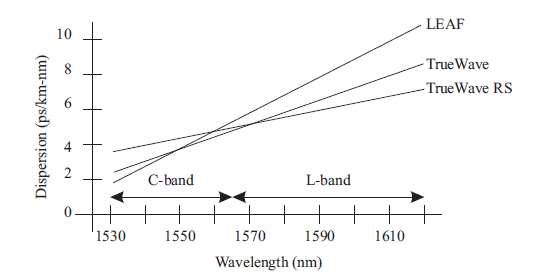
\includegraphics[width=260.3pt]{images/image88.png}
\end{center}
\end{frame}

\section[Δομικά Στοιχεία]{Μέρος 3$^{\text{ο}}$: Δομικά οπτικά στοιχεία}
\begin{frame}
\vfill
\begin{center}
{\Large\structure{Μέρος 3$^{\text{ο}}$: Δομικά οπτικά στοιχεία}}
\end{center}
\vfill
\end{frame}

\begin{frame}[shrink=20,t]{Συζεύκτες (Couplers)}
\begin{itemize}
\item Για παράδειγμα μπορούνε να συνδυάσουνε δύο σήματα, ένα στα 1550nm και ένα στα 1310nm τα οποία εισάγονται στις δύο θύρες εισόδου
\item Τα σήματα αυτά μπορούνε να παρουσιαστούνε σε μία έξοδο του συζεύκτη μαζί και να εισέρθουνε σε μία οπτική ίνα (πολυπλεξία).
\item Χρησιμοποιούνται (όπως θα δούμε) για την κατασκευή συμβολομέτρων.
\item Επίσης χρησιμοποιούνται για την υλοποίηση “tap” όπου ένα μικρό μέρος της ισχύος που βρίσκεται σε μία θύρα εισόδου οδηγείται στην δεύτερη θύρα εξόδου ενώ το υπόλοιπο παρουσιάζεται  στην πρώτη.
\item Επειδή ο συζεύκτης δεν είναι ιδανικός μπορεί να έχουμε απώλειες εισαγωγής (insertion loss) και απώλειες πόλωσης (polarization dependent loss).
\end{itemize}
\medskip
\begin{itemize}
\item Χρησιμοποιείται για να μεταφέρει ένα μέρος της ισχύος από τις θύρες εισόδου στις θύρες εξόδου.
\item Οι συζεύκτες μπορούνε να σχεδιαστούνε ώστε να έχουνε και εξάρτηση από το μήκος κύματος
\end{itemize}
\begin{center}
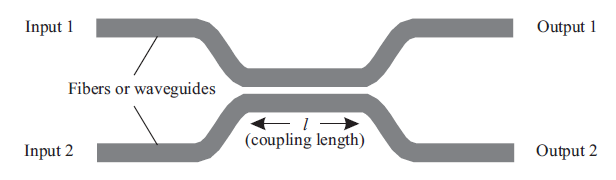
\includegraphics[width=338.3pt]{images/image89.png}
\end{center}
\end{frame}

\begin{frame}[shrink=20,t]{Περιγραφή της λειτουργία του συζεύκτη}
\begin{itemize}
\item Κάθε κυματοδηγός (απουσία του άλλου) υποστηρίζει έναν τρόπο διάδοσης με σταθερά διάδοσης \textit{β}
\item Παρουσία του άλλου κυματοδηγού έχουμε σύζευξη (coupling) τρόπων.
\item Αυτό έχει ως αποτέλεσμα ένα μέρος του πεδίου να μεταφέρεται από τον ένα κυματοδηγό στον άλλο.
\item Η διαδικασία χαρακτηρίζεται από τον συντελεστή σύζευξης κ. Όσο πιο κοντά είναι κυματοδηγοί τόσο μεγαλύτερο είναι το κ και τόσο πιο ισχυρή είναι η σύζευξη.
\item Ανάλογα με το μήκος \textit{l} μπορεί να μεταφέρεται:
\begin{itemize}
\item όλη η ισχύς από την θύρα εισόδου “1” στη θύρα εξόδου “2”
\item μηδενική ισχύς από την θύρα εισόδου “1” στη θύρα εξόδου “2”
\item μισή ισχύς από την θύρα “1” στη θύρα “2” (η άλλη μισή εμφανίζεται στην “1”)
\end{itemize}
\end{itemize}
\begin{center}
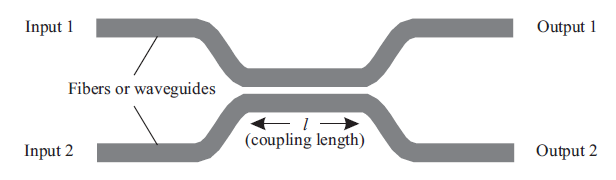
\includegraphics[width=338.3pt]{images/image89.png}
\end{center}
\begin{center}
$\displaystyle \begin{bmatrix}E_{o1}(f)\\E_{o2}(f)\end{bmatrix}=e^{-j\beta l}\begin{bmatrix}\cos(\kappa l)&j\sin(\kappa l)\\j\sin(\kappa l)&\cos(\kappa l)\end{bmatrix}\begin{bmatrix}E_{i1}(f)\\E_{i2}(f)\end{bmatrix}$\\[0.6ex]
\end{center}
\end{frame}

\begin{frame}[shrink=10,t]{Μεγαλύτεροι Συζεύκτες}
\begin{center}
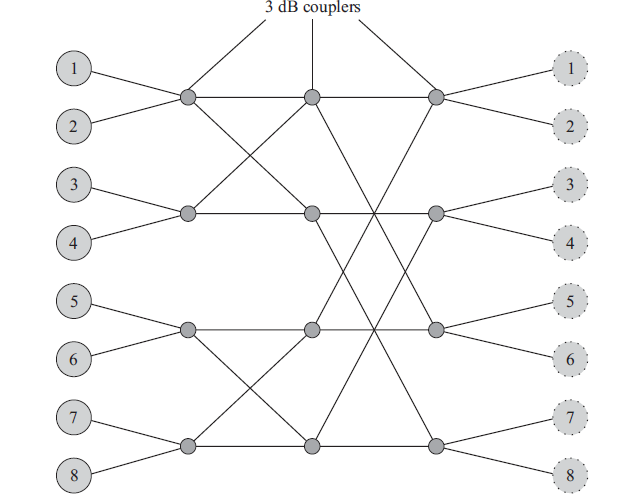
\includegraphics[width=249.7pt]{images/image91.png}
\end{center}
\end{frame}

\begin{frame}[shrink=10,t]{Κυκλοφορητές (Circulators)}
\begin{itemize}
\item Επιτρέπουν την διάδοση προς μία μονάχα διεύθυνση.
\item Χρησιμοποιούνται σε περιπτώσεις που πρέπει να ελαχιστοποιήσουμε τις ανακλάσεις.
\item Βασίζονται σε απομονωτές (isolators)
\end{itemize}
\begin{center}
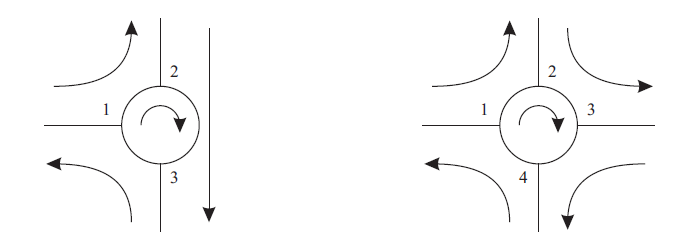
\includegraphics[width=338.3pt]{images/image92.png}
\end{center}
\end{frame}

\begin{frame}[shrink=20,t]{Απομονωτές}
\begin{itemize}
\item Οι απομονωτές βασίζονται στους στροφείς Faraday.
\item Οι στροφείς Faraday περιστρέφουν τον επίπεδο πόλωσης του φωτός κατά μία γωνία θ.
\item Η γωνία \textit{θ} όμως είναι ανεξάρτητη από το αν το φως εισέρχεται στη διάταξη από αριστερά προς δεξιά ή από δεξιά προς τα αριστερά.
\item Με αυτό τον τρόπο το φως που εισέρχεται στην δεξιά θύρα του απομονωτή περνάει από τον πρώτο ελεγκτή πόλωσης.
\item Στη συνέχεια στρέφεται κατά π/4 και περνάει από τον δεύτερο ελεγκτή πόλωσης.
\item Το φως που ανακλάται από την έξοδο περνάει πάλι από τον δεύτερο ελεγκτή και στη συνέχεια ξαναπερνάει από τον στροφέα Faraday.
\item Η πόλωση του έχει τώρα γυρίσει σε γωνία π/2 και επομένως δεν μπορεί να περάσει από τον πρώτο ελεγκτή πόλωσης.
\item Υπάρχει τρόπος να σχεδιαστεί ο απομονωτής ώστε να λειτουργεί με αυθαίρετη πόλωση εισόδου.
\end{itemize}
\begin{center}
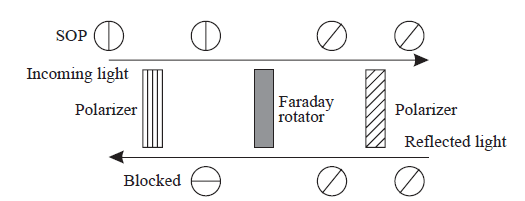
\includegraphics[width=223.3pt]{images/image93.png} 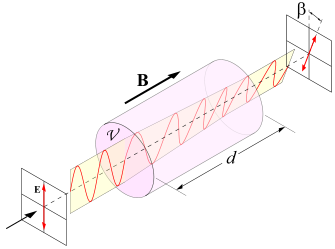
\includegraphics[width=115.0pt]{images/image94.png}
\end{center}
\end{frame}

\begin{frame}[shrink=10,t]{Απομονωτής ανεξάρτητος από πόλωση (*)}
\begin{itemize}
\item SWP=Spatial walk off polarizer. Χωρίζει το φως σε δύο ορθογώνιες γραμμικές πολώσεις.
\end{itemize}
\medskip
\begin{itemize}
\item Διάδοση από τα αριστερά στα δεξιά
\end{itemize}
\medskip
\begin{itemize}
\item Διάδοση από τα δεξιά στα αριστερά.
\end{itemize}
\begin{center}
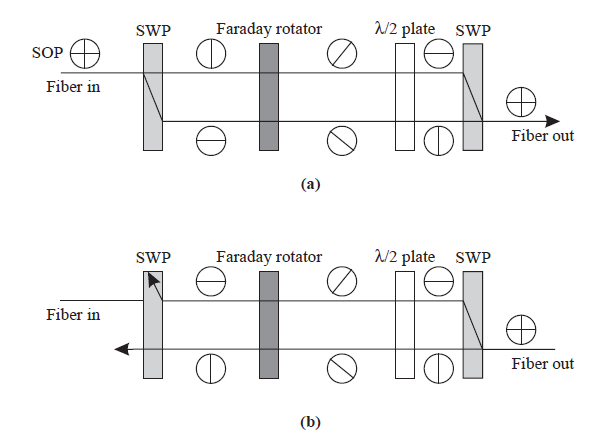
\includegraphics[width=203.8pt]{images/image95.png}
\end{center}
\end{frame}

\begin{frame}[shrink=10,t]{Οπτικά Φίλτρα}
\begin{itemize}
\item Απαιτήσεις:
\begin{itemize}
\item Μικρές απώλειες εισαγωγής
\item Ανεξαρτησία από πόλωση
\item Ανεξαρτησία από θερμοκρασία
\item Ομαλή (flat) απόκριση γύρω από την κεντρική συχνότητα
\item Μικρό επίπεδο διαφωνίας (crosstalk)
\item Κόστος!!!
\end{itemize}
\end{itemize}
\begin{center}
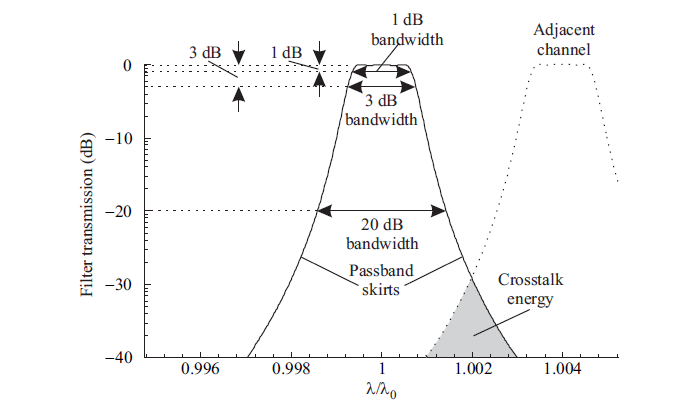
\includegraphics[width=205.6pt]{images/image96.png}
\end{center}
\end{frame}

\begin{frame}[shrink=10,t]{Χαρακτηριστικά Τεχνολογιών}
\begin{itemize}
\item AWG = Arrayed waveguide grating
\item TFMF= Thin film multi-cavity filter
\end{itemize}
\begin{center}
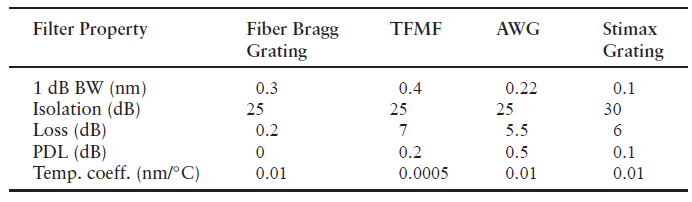
\includegraphics[width=338.3pt]{images/image97.png}
\end{center}
\end{frame}

\begin{frame}[shrink=20,t]{Τεχνολογίες Φίλτρων: Φράγματα}
\begin{itemize}
\item Μπορεί κανείς να δείξει ότι αν \textit{a}(sin\textit{θ}$_{\text{\textit{i}}}$-sin\textit{θ}$_{\text{\textit{d}}}$)=\textit{m}\textit{λ}\textit{ }τότε τα δευτερεύοντα κύματα συμβάλλουν προσθετικά (με διαφορά φάσης πολλαπλάσια του 2π).
\item To \textit{m} είναι ένας ακέραιος που ονομάζεται η τάξη του φράγματος.
\item Για \textit{m}>0 βλέπουμε πως η γωνία \textit{θ}$_{\text{\textit{d}}}$ εξαρτάται από το μήκος κύματος.
\item Ωστόσο για m=0 αυτό δεν συμβαίνει (έχουμε θi=θd) και για το λόγω αυτό κατασκευάζουμε κατάλληλα το φράγμα με την τεχνική του blazing.
\end{itemize}
\medskip
\begin{itemize}
\item Με τον όρο φράγμα εννοούμε οποιαδήποτε δομή επιτρέπει την υπέρθεση κυμάτων που έχουν προκύψει από το ίδιο αρχικό κύμα με κάποια διαφορά φάσης.
\item Παρακάτω βλέπουμε φράγματα που αποτελούνται από σχισμές.
\item Κάθε σχισμή δρα ως μία δευτερεύουσα πηγή και τα κύματα που γεννιούνται μπορεί να συμβάλουν καταστροφικά ή προσθετικά.
\end{itemize}
\begin{center}
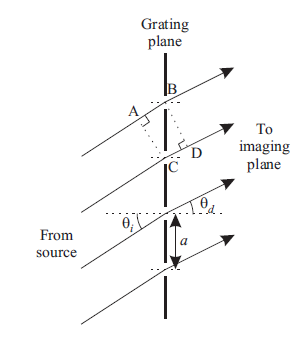
\includegraphics[width=64.3pt]{images/image98.png} 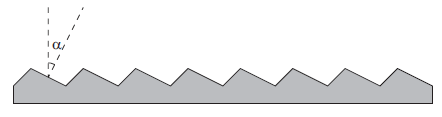
\includegraphics[width=274.0pt]{images/image99.png}
\end{center}
\end{frame}

\begin{frame}[shrink=20,t]{Φράγματα Bragg}
\begin{itemize}
\item Χρησιμοποιούνται αρκετά συχνά στα οπτικά συστήματα.
\item Ας υποθέσουμε πως σε ένα κυματοδηγό έχουμε “γράψει” ένα φράγμα με περίοδο Λ.
\item Το φράγμα προκαλεί σύζευξη μεταξύ των τρόπων του κυματοδηγού
\item Η σύζευξη μεγιστοποιείται όταν ισχύει η συνθήκη Bragg, 2π/Λ=|\textit{β}$_{\text{0}}$-\textit{β}$_{\text{1}}$| όπου \textit{β}$_{\text{0}}$ και \textit{β}$_{\text{1}}$ είναι οι σταθερές διάδοσης των τρόπων.
\item Σε έναν κυματοδηγό, για κάθε τρόπο με σταθερά διάδοσης \textit{β}$_{\text{0}}$\textit{=2}π\textit{n}$_{\text{eff}}$\textit{/}\textit{λ} υπάρχει και ένας τρόπος με σταθερά διάδοσης –\textit{β}$_{\text{0}}$ που διαδίδεται προς τα πίσω.
\item Στην περίπτωση αυτή η συνθήκη Bragg γράφεται: λ=2\textit{n}$_{\text{eff}}$Λ
\item Το μήκος κύματος αυτό ονομάζεται μήκος κύματος Bragg
\end{itemize}
\begin{center}
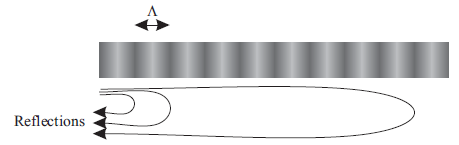
\includegraphics[width=338.3pt]{images/image100.png}
\end{center}
\end{frame}

\begin{frame}[shrink=10,t]{Φράγματα Bragg: Συνάρτηση Μεταφοράς}
\begin{center}
\setlength{\unitlength}{0.000060pt}
\begin{picture}(4757323,3034768)
\put(0,0){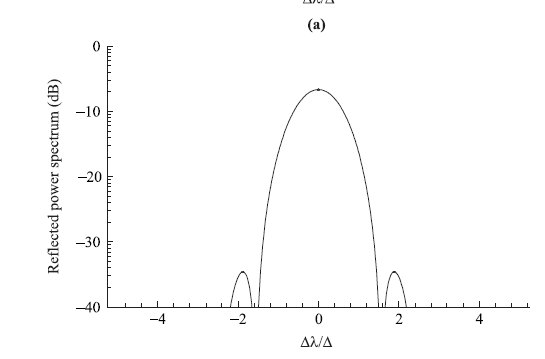
\includegraphics[width=285.3pt]{images/image102.png}}
\put(0,1058632){\footnotesize \shortstack{Κανονικό Φράγμα}}
\put(1971102,3034768){\footnotesize \shortstack{Apodized Φράγμα}}
\end{picture}
\end{center}
\end{frame}

\begin{frame}[shrink=20,t]{Φράγματα Bragg σε οπτικές ίνες}
\begin{itemize}
\item Μπορούμε να γράψουμε φράγματα Bragg σε οπτικές ίνες.
\item Τα φίλτρα αυτά έχουνε χαμηλές απώλειες (0.1dB) χαμηλή διαφωνία (-40dB), καλή θερμική σταθερότητα (με ειδικές τεχνικές πετυχαίνουμε 0.07\ensuremath{\times}10$^{-2}$nm/$^{\text{o}}$C)
\item Μπορούνε να χρησιμοποιηθούνε για add/drop multiplexers όπως δείχνει και η παραπάνω εικόνα.
\end{itemize}
\begin{center}
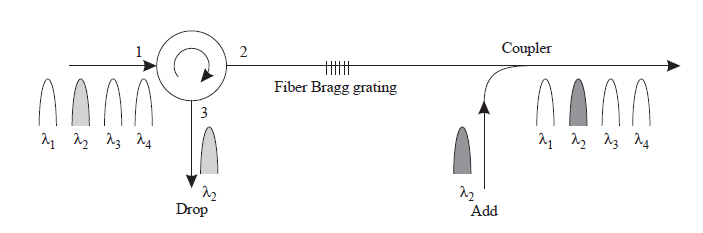
\includegraphics[width=338.3pt]{images/image103.png}
\end{center}
\end{frame}

\begin{frame}[shrink=20,t]{Φίλτρα Fabry-Perot}
\begin{itemize}
\item Στην παραπάνω σχέση \textit{Α} είναι οι απώλειες του κάθε καθρέφτη, \textit{R} η ανακλαστικότητα τους, \textit{τ}=\textit{nl}/\textit{c} όπου \textit{n} είναι ο δείκτης διάθλασης της κοιλότητας και \textit{l} το μήκος της.
\item Η συνάρτηση μεταφοράς είναι περιοδική με περίοδο FSR=1/2/\textit{τ}
\item Τα αρχικά FSR σημαίνουν free spectral range.
\end{itemize}
\begin{center}
\setlength{\unitlength}{0.000077pt}
\begin{picture}(4543425,1952625)
\put(0,0){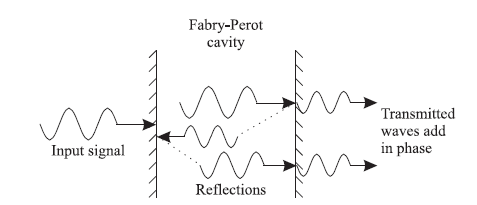
\includegraphics[width=349.0pt]{images/image105.png}}
\end{picture}
\end{center}
\centering\footnotesize Αποτελούνται από δύο υψηλής ανακλαστικότητας \textit{R} κάτοπτρα. Εντός της κοιλότητας Fabry Perot συμβάλλουν κύματα που προέρχονται από διαδοχικές ανακλάσεις στα κάτοπτρα. Η απόκριση του φίλτρου δίνεται από την εξίσωση:\par
\normalsize
\begin{center}
$\displaystyle T_{\mathrm{FP}}(f)=\frac{\left[1-\dfrac{A}{1-R}\right]^{2}}{1+\left[\dfrac{2\sqrt{R}}{1-R}\sin(2\pi f\tau)\right]^{2}}$\\[0.6ex]
\end{center}
\end{frame}

\begin{frame}[shrink=10,t]{Φίλτρα διηλεκτρικών κοιλοτήτων}
\begin{center}
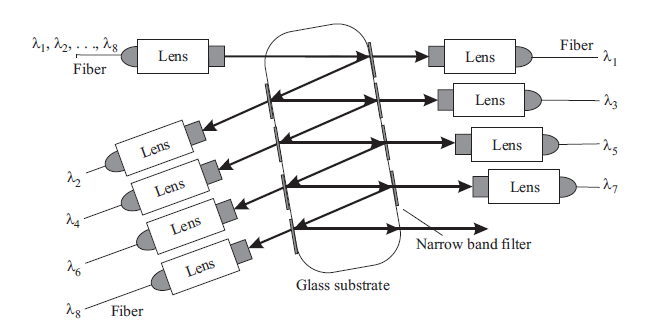
\includegraphics[width=177.4pt]{images/image107.png} 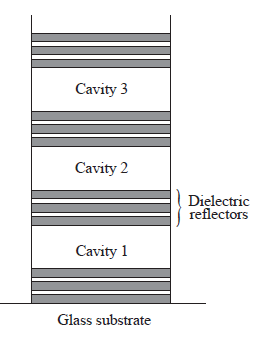
\includegraphics[width=69.4pt]{images/image108.png} 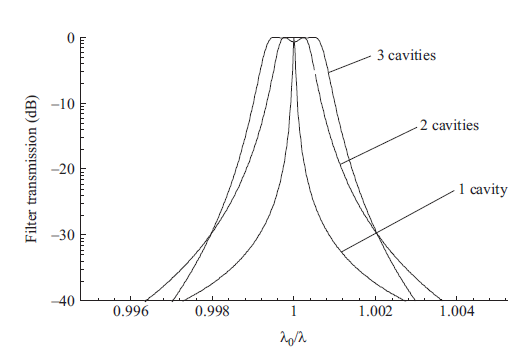
\includegraphics[width=131.3pt]{images/image109.png}
\end{center}
\end{frame}

\begin{frame}[shrink=20,t]{Φίλτρο Mach-Zehnder (Συμβολόμετρο)}
\begin{itemize}
\item Στην περίπτωση που έχουμε μία είσοδο:
\end{itemize}
\begin{center}
\setlength{\unitlength}{0.000066pt}
\begin{picture}(5457825,1914525)
\put(0,0){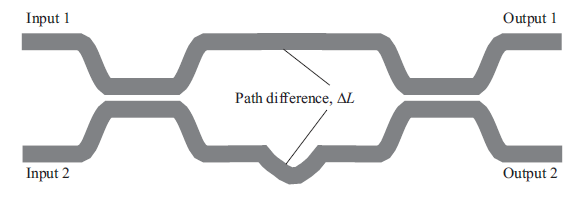
\includegraphics[width=358.2pt]{images/image112.png}}
\put(1345580,0){\footnotesize \shortstack{1$^{\text{ος}}$ συζεύκτης}}
\put(2895236,0){\footnotesize \shortstack{Διαφορά Δρόμου}}
\end{picture}
\end{center}
\begin{center}
$\displaystyle \begin{bmatrix}E_{o1}(f)\\E_{o2}(f)\end{bmatrix}=e^{-j\beta(2l+L)}\begin{bmatrix}1/\sqrt{2}&j/\sqrt{2}\\j/\sqrt{2}&1/\sqrt{2}\end{bmatrix}\begin{bmatrix}1&0\\0&e^{j\beta\Delta L}\end{bmatrix}\begin{bmatrix}1/\sqrt{2}&j/\sqrt{2}\\j/\sqrt{2}&1/\sqrt{2}\end{bmatrix}\begin{bmatrix}E_{i1}(f)\\E_{i2}(f)\end{bmatrix}$\\[0.6ex]
$\displaystyle \begin{bmatrix}T_{1}(f)\\T_{2}(f)\end{bmatrix}=\begin{bmatrix}|E_{o1}(f)/E_{i1}(f)|^{2}\\|E_{o2}(f)/E_{i1}(f)|^{2}\end{bmatrix}=\begin{bmatrix}\sin^{2}(\beta\Delta L/2)\\\cos^{2}(\beta\Delta L/2)\end{bmatrix}$\\[0.6ex]
\end{center}
\end{frame}

\begin{frame}[shrink=10,t]{Mach-Zehnder πολλαπλών σταδίων}
\begin{center}
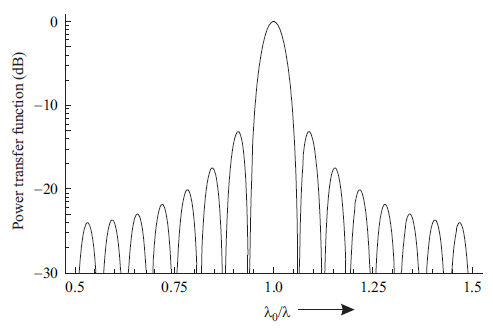
\includegraphics[width=63.0pt]{images/image113.png} 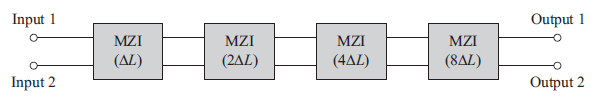
\includegraphics[width=261.9pt]{images/image114.png} 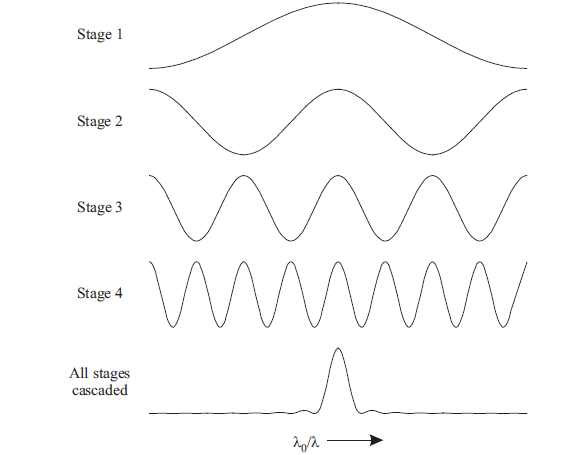
\includegraphics[width=53.2pt]{images/image115.png}
\end{center}
\end{frame}

\begin{frame}[shrink=10,t]{Arrayed Waveguide Grating (AWG)}
\begin{center}
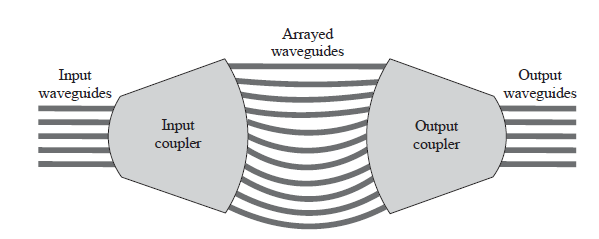
\includegraphics[width=158.8pt]{images/image116.png} 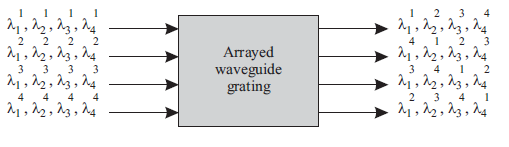
\includegraphics[width=219.3pt]{images/image117.png}
\end{center}
\end{frame}

\begin{frame}[shrink=10,t]{Αποπολυπλέκτες με πολλά μήκη κύματος}
\begin{itemize}
\item Για την υλοποίηση μεγαλύτερων αποπολυπλεκτών μπορούμε να χρησιμοποιήσουμε AWG.
\item Eμπορικά διαθέσιμα είναι AWG 40\ensuremath{\times}40 και ίσως και λίγο μεγαλύτεροι.
\item Εναλλακτικά μπορούμε να συνδυάσουμε μικρότερους αποπολυπλέκτες.
\begin{itemize}
\item multistage banding (αποπολυπλέκτες πολλαπλών σταδίων, κάθε στάδιο αποπολυπλέκει μία ομάδα γειτονικών μηκών κύματος).
\item multistage interleaving (αποπολυπλέκτες πολλαπλών σταδίων, κάθε στάδιο αποπολυπλέκει μία ομάδα μηκών κύματος που απέχει μεγαλύτερη απόσταση).
\end{itemize}
\end{itemize}
\end{frame}

\begin{frame}[shrink=10,t]{Multistage banding}
\begin{center}
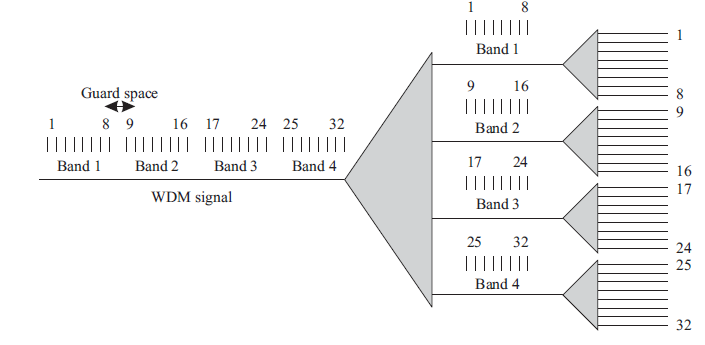
\includegraphics[width=378.1pt]{images/image118.png}
\end{center}
\end{frame}

\begin{frame}[shrink=10,t]{Multistage interleaving}
\begin{center}
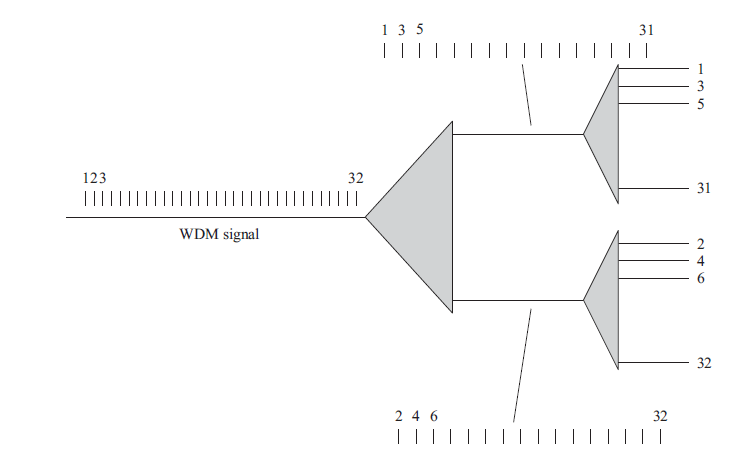
\includegraphics[width=314.9pt]{images/image119.png}
\end{center}
\end{frame}

\begin{frame}[shrink=20,t]{Οπτικοί Ενισχυτές}
\begin{itemize}
\item Οι οπτικές απώλειες (ίνας + δομικών στοιχείων) μειώνουνε την ισχύ του σήματος
\item Αν οι απώλειες είναι πολύ μεγάλες τότε ο δέκτης δεν μπορεί να ξεχωρίσει το σήμα από το θόρυβο.
\item Στα παλιότερα συστήματα, το πρόβλημα λυνότανε τοποθετώντας αναγεννητές ενδιάμεσα του πομπού και του δέκτη.
\item Ο αναγεννητής μετατρέπει το οπτικό σήμα σε ηλεκτρονικό και το ξαναεκπέμπει σε οπτική μορφή \textit{αναγεννημένο}.
\item Οι οπτικοί ενισχυτές ενισχύουν το σήμα σε καθαρά οπτική μορφή. Επομένως ένας ενισχυτής:
\begin{itemize}
\item μπορεί να ενισχύσει πολλά κανάλια WDM
\item μπορεί να  ενισχύσει σήματα ανεξάρτητα του ρυθμού
\item μπορεί να ενισχύσει ένα σήμα ανεξαρτήτως σχήματος διαμόρφωσης
\end{itemize}
\item Φυσικά οι οπτικοί ενισχυτές δεν είναι ιδανικοί:
\begin{itemize}
\item εισάγουν θόρυβο
\item δεν έχουν ομαλή φασματική απόκριση
\item το κέρδος εξαρτάται και από την ισχύ εισόδου
\end{itemize}
\end{itemize}
\end{frame}

\begin{frame}[shrink=20,t]{Αλληλεπίδραση Ύλης-Φωτός}
\begin{itemize}
\item Αυθόρμητη εκπομπή (\textit{spontaneous emission}): Ένα φωτόνιο εκπέμπεται (τυχαία) εξαιτίας της αποδιέγερσης ενός ηλεκτρονίου από μία κατάσταση υψηλής ενέργειας (\textit{Ε}$_{\text{2}}$) σε μία κατάσταση χαμηλής ενέργειας (\textit{Ε}$_{\text{1}}$).
\item Στην περίπτωση της εξαναγκασμένης εκπομπής (\textit{stimulated emission}) η μετάβαση αυτή υποβοηθείται από ένα αρχικό φωτόνιο. Το φωτόνιο που γεννάται είναι όμοιο με το αρχικό.
\item Σε κάθε περίπτωση η ενέργεια του φωτονίου είναι \textit{hf}=\textit{E}$_{\text{2}}$-\textit{E}$_{\text{1}}$
\end{itemize}
\begin{center}
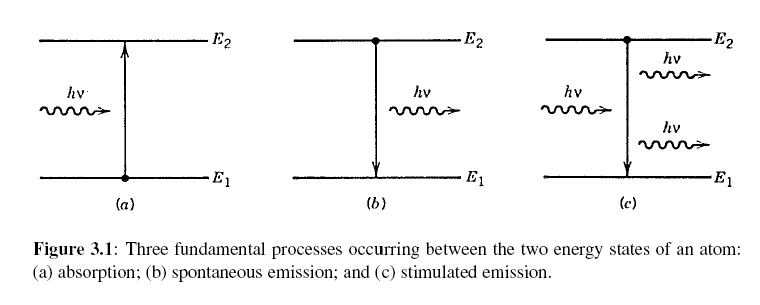
\includegraphics[width=338.3pt]{images/image120.png}
\end{center}
\end{frame}

\begin{frame}[shrink=20,t]{Eξαναγκασμένη και Αυθόρμητη Εκπομπή}
\begin{itemize}
\item Ρυθμοί απορρόφησης και εκπομπής
\begin{itemize}
\item Αυθόρμητη εκπομπή: \textit{R}$_{\text{spon}}$=\textit{AN}$_{\text{2}}$ όπου \textit{Ν}$_{\text{2}}$ η πυκνότητα των φορέων στη στάθμη \textit{Ε}$_{\text{2}}$.
\item Εξαναγκασμένη εκπομπή: \textit{R}$_{\text{stim}}$=\textit{B}\textit{ρ}\textit{N}$_{\text{2}}$ όπου \textit{ρ} είναι η πυκνότητα φωτονίων.
\item Απορρόφηση: \textit{R}$_{\text{abs}}$=\textit{C}\textit{ρ}\textit{N}$_{\text{1}}$ όπου \textit{Ν}$_{\text{1}}$ η πυκνότητα των φορέων στη στάθμη \textit{Ε}$_{\text{1}}$\textit{.}
\end{itemize}
\item Θεωρούμε πως βρισκόμαστε σε κατάσταση θερμικής ισορροπίας, οπότε
\begin{itemize}
\item d\textit{N}$_{\text{1}}$/d\textit{t}=d\textit{N}$_{\text{2}}$/d\textit{t}=0.
\item \textit{AN}$_{\text{2}}$+\textit{B}\textit{ρΝ}$_{\text{2}}$=\textit{C}\textit{ρΝ}$_{\text{1}}$
\item \textit{Ν}$_{\text{2}}$/\textit{Ν}$_{\text{1}}$=exp(-\textit{hf}/\textit{k}$_{\text{B}}$\textit{T}).
\end{itemize}
\item Από τις παραπάνω εξισώσεις συνάγουμε ότι: \textit{ρ}=(\textit{Α}/\textit{Β})(\textit{C}/\textit{B}exp(-\textit{hf}/\textit{k}$_{\text{\textit{B}}}$\textit{T})-1)$^{\text{-1}}$ το οποίο πρέπει να συμφωνεί με την εξίσωση του Planck \textit{ρ}=(8π\textit{hf}$^{\text{3}}$)/\textit{c}$^{\text{3}}$(exp(-\textit{hf}/\textit{k}$_{\text{\textit{B}}}$\textit{T})-1)$^{\text{-1}}$.
\item Αυτό συμβαίνει όταν:
\begin{itemize}
\item Α=(8π\textit{hf}$^{\text{3}}$)/\textit{c}$^{\text{3}}$\textit{B.}
\item \textit{C=B}
\item Οι σχέσεις αυτές είναι γνωστές ως σχέσεις Einstein.
\end{itemize}
\end{itemize}
\end{frame}

\begin{frame}[shrink=20,t]{Eξαναγκασμένη και Αυθόρμητη Εκπομπή}
\begin{itemize}
\item Σε κατάσταση θερμικής ισορροπίας \textit{R}$_{\text{stim}}$/\textit{R}$_{\text{spon}}$= (exp(-\textit{hf}/\textit{k}$_{\text{\textit{B}}}$\textit{T})-1)$^{\text{-1}}$. Για τιμές του f στο υπέρυθρο ή το ορατό φάσμα, \textit{R}$_{\text{stim}}$/\textit{R}$_{\text{spon}}$<<1, οπότε η αυθόρμητη εκπομπή υπερισχύει.
\item Πότε η εξαναγκασμένη εκπομπή γίνεται σημαντική;
\item Καταρχήν θα πρέπει να υπερνικήσει την απορρόφηση, δηλαδή \textit{R}$_{\text{stim}}$>\textit{R}$_{\text{abs}}$.
\item Αυτό μεταφράζεται σε \textit{Ν}$_{\text{2}}$>\textit{Ν}$_{\text{1}}$ κάτι που σίγουρα δεν ισχύει σε κατάσταση θερμικής ισορροπίας.
\item Η παραπάνω συνθήκη ονομάζεται αναστροφή πληθυσμών (population inversion).
\item Είναι η βασική προϋπόθεση για να έχουμε οπτική ενίσχυση και δράση LASER (Light Amplification by Stimulated Emission of Radiation).
\item Σε ατομικά συστήματα (π.χ. αέρια) επιτυγχάνεται με οπτικό τρόπο (μέσω άλλων μεταβάσεων).
\item Στην περίπτωση των ημιαγωγών, πάλι έχουμε εξαναγκασμένη και αυθόρμητη εκπομπή αλλά η περιγραφή είναι ελαφρώς διαφορετική. Τα βασικά όμως συμπεράσματα ισχύουν.
\end{itemize}
\end{frame}

\begin{frame}[shrink=20,t]{Eξαναγκασμένη και Αυθόρμητη Εκπομπή}
\begin{itemize}
\item Στην περίπτωση της εξαναγκασμένης εκπομπής όλα τα φωτόνια που παράγονται έχουν τα ίδια χαρακτηριστικά και επομένως την ίδια φάση.
\item Πρόκειται για \textit{σύμφωνο} φως. Το πεδίο χαρακτηρίζεται από το πλάτος του και την  φάση του.
\item Στη περίπτωση της αυθόρμητης εκπομπής έχουμε \textit{ασύμφωνο} φως.
\item Δηλαδή τα φωτόνια μπορεί να έχουνε διαφορετική, τυχαία φάση.
\item Όταν συμβάλλει ένας μεγάλος αριθμός φωτονίων με τυχαία φάση έχουμε την άθροιση πολλών μικρών πεδίων.
\item H ισχύς του πεδίου είναι |\ensuremath{\sum}$_{\text{\textit{m}}}$exp(\textit{j}\textit{φ}$_{\text{\textit{m}}}$)|$^{\text{2}}$=\ensuremath{\sum}$_{\text{\textit{μν}}}$exp(\textit{j}\textit{φ}$_{\text{\textit{μ}}}$\textit{-}\textit{j}\textit{φ}$_{\text{\textit{ν}}}$)\ensuremath{\cong}\textit{Μ}\textit{. }
\item Επομένως κατά την συμβολή δύο ασύμφωνων πεδίων δεν παίζει ρόλο καθόλου η φάση του φωτός και απλά αθροίζουμε την ισχύ, δηλαδή \textit{P}$_{\text{tot}}$=\textit{P}$_{\text{1}}$+\textit{P}$_{\text{2}}$=|\textit{Ε}$_{\text{1}}$|$^{\text{2}}$+|\textit{Ε}$_{\text{2}}$|$^{\text{2}}$
\item Κατά την συμβολή σύμφωνων πεδίων παίζει ρόλο η φάση: \textit{P}$_{\text{tot}}$=|\textit{E}$_{\text{1}}$exp(\textit{j}\textit{φ}$_{\text{1}}$)+\textit{E}$_{\text{2}}$exp(\textit{j}\textit{φ}$_{\text{2}}$)|$^{\text{2}}$=|\textit{E}$_{\text{1}}$|$^{\text{2}}$+|\textit{E}$_{\text{2}}$|$^{\text{2}}$+2\textit{E}$_{\text{1}}$\textit{E}$_{\text{2}}$cos(\textit{φ}$_{\text{1}}$-\textit{φ}$_{\text{2}}$).\textit{ }
\end{itemize}
\end{frame}

\begin{frame}[shrink=20,t]{Οι οπτικοί ενισχυτές ίνας Ερβίου}
\begin{itemize}
\item EDFA = Erbium Doped Fiber Amplifier, ενισχυτής ίνας ντοπαρισμένης με ιόντα Ερβίου.
\item Δηλαδή πρόκειται για μία οπτική ίνα στην οποία έχουμε τοποθετήσει ιόντα ρβίου (Er$^{\text{3+}}$).
\item Με αυτόν τον τρόπο πετυχαίνουμε μία πολύ καλή συμφωνία: χρησιμοποιούμε ένα laser (pump) στα 980nm ή στα 1480nm για να προκαλέσουμε αναστροφή πληθυσμών.
\item Μέσω της εξαναγκασμένης εκπομπής μπορούμε να ενισχύσουμε ένα σήμα στα 1550nm.
\item Ο EDFA έχει κυριαρχήσει στα οπτικά συστήματα εξαιτίας:
\begin{itemize}
\item της διαθεσιμότητας pump lasers στις συχνότητες αυτές με υψηλή ισχύ.
\item πρόκειται για μία διάταξη με οπτική ίνα \ensuremath{\rightarrow} ανεξαρτησία από πόλωση και εύκολη σύζευξη με ίνα.
\item δεν απαιτεί ιδιαίτερο χειρισμό, είναι σχετικά απλή διάταξη.
\item δεν εισάγει διαφωνία όταν ενισχύει κανάλια WDM.
\end{itemize}
\end{itemize}
\end{frame}

\begin{frame}[shrink=20,t]{Ενεργειακές Καταστάσεις του Ερβίου}
\begin{itemize}
\item Όταν το ιόν του Ερβίου δεν αλληλεπιδρά με άλλα άτομα τότε υπάρχουν τέσσερις διακριτές στάθμες που μας ενδιαφέρουν (\textit{Ε}$_{\text{1}}$,…,\textit{Ε}$_{\text{4}}$).
\item Παρουσία του γυαλιού (SiO2), οι ενεργειακές στάθμες διασπώνται σε πολλές επιμέρους στάθμες γύρω από τις αρχικές.
\item Αυτή η διαδικασία ονομάζεται διάσπαση Stark.
\item Επειδή το γυαλί είναι άμορφο, οι στάθμες αυτές διαφέρουν από ιόν σε ιόν και επομένως παρουσιάζονται σαν συνεχείς ενεργειακές ζώνες.
\item Στην περίπτωση του EDFA μας ενδιαφέρει πολύ η μετάβαση από το Ε2 στο Ε1 που παράγει φωτόνια στα 1525-1570nm που συμπίπτει με την περιοχή όπου οι απώλειες των ινών είναι πολύ μικρές.
\end{itemize}
\begin{center}
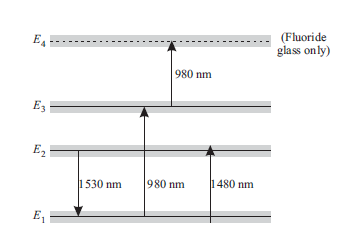
\includegraphics[width=219.5pt]{images/image121.png}
\end{center}
\end{frame}

\begin{frame}[shrink=20,t]{Ενεργειακές Καταστάσεις του Ερβίου}
\begin{itemize}
\item Σε κατάσταση θερμικής ισορροπίας έχουμε \textit{Ν}$_{\text{1}}$>\textit{Ν}$_{\text{2}}$>\textit{Ν}$_{\text{3}}$.
\item Για να ενισχύσουμε το σήμα θα πρέπει η εξαναγκασμένη εκπομπή να υπερισχύει της απορρόφησης γύρω στα 1.55μm.
\item οπότε θα πρέπει \textit{Ν}$_{\text{2}}$>\textit{Ν}$_{\text{1}}$ (αναστροφή πληθυσμών).
\item Για να επιτύχουμε την παραπάνω συνθήκη χρησιμοποιούμε ένα laser στα 980nm που διεγείρει τα ιόντα από την \textit{Ε}$_{\text{1}}$ στην \textit{Ε}$_{\text{3}}$ μέσω της απορρόφησης.
\item Η διαδικασία αυτή ονομάζεται \textit{άντληση} (pumping).
\item Τα ιόντα που βρίσκονται στην \textit{Ε}$_{\text{3}}$ έχουν την τάση να αποδιεγείρονται στην \textit{Ε}$_{\text{2}}$ σε σύντομο χρονικό διάστημα (\textit{τ}$_{\text{32}}$\ensuremath{\cong}1μs).
\item Ωστόσο τα ιόντα που βρίσκονται στο \textit{Ε}$_{\text{2}}$ αργούν να αποδιεγερθούν και να πέσουν στην \textit{Ε}$_{\text{1}}$ (\textit{τ}$_{\text{21}}$=10ms). Άλλωστε και να συμβεί αυτό θα διεγερθούν εξαιτίας της άντλησης ξανά στην \textit{Ε}$_{\text{3}}$.
\end{itemize}
\begin{center}
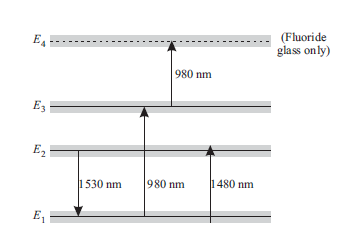
\includegraphics[width=219.5pt]{images/image121.png}
\end{center}
\end{frame}

\begin{frame}[shrink=20,t]{Η δομή ενός EDFA}
\begin{itemize}
\item Εναλλακτικά θα μπορούσαμε να κάνουμε άντληση και στα 1480nm (κάτω άκρο της στάθμης γύρω από το Ε1).
\begin{itemize}
\item Ωστόσο η άντληση δεν είναι τόσο αποδοτική όσο στα 980nm (μικρότερη αναστροφή πληθυσμών).
\item Μεγαλύτερος θόρυβος (μικρότερη αναστροφή πληθυσμών).
\item Όμως μπορούμε να υλοποιήσουμε πηγές με περισσότερη ισχύ στα 1480nm.
\item Επίσης στα 1480nm η ίνα έχει σχετικά χαμηλές απώλειες οπότε το σήμα άντλησης μπορεί να έρχεται από μακριά (remote pumping).
\end{itemize}
\end{itemize}
\begin{center}
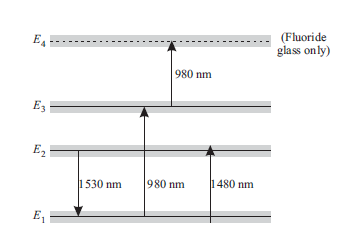
\includegraphics[width=111.3pt]{images/image121.png} 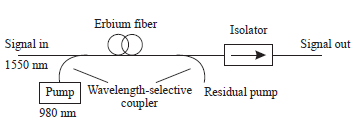
\includegraphics[width=227.0pt]{images/image122.png}
\end{center}
\end{frame}

\begin{frame}[shrink=20,t]{Το κέρδος του ενισχυτή EDFA}
\begin{itemize}
\item Τα ιόντα δεν αποικούν ομοιόμορφα τις ενεργειακές ζώνες και επομένως το κέρδος του ενισχυτή παρουσιάζει εξάρτηση από την συχνότητα.
\item Αυτό σημαίνει πως σε ένα σύστημα WDM κάποια κανάλια θα ενισχύονται παραπάνω από κάποια άλλα.
\item Αυτό δεν είναι συχνά αποδεκτό και υπάρχουνε διάφορες τεχνικές για την ισοστάθμιση του κέρδους (φίλτρα ή χρήση ειδικού γυαλιού fluoride glass)
\end{itemize}
\begin{center}
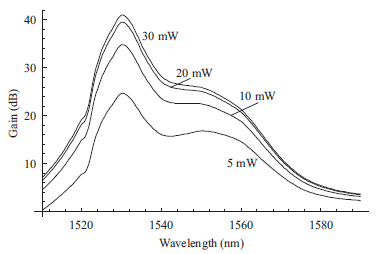
\includegraphics[width=224.4pt]{images/image123.png}
\end{center}
\end{frame}

\begin{frame}[shrink=20,t]{EDFA δύο σταδίων}
\begin{itemize}
\item Το πρώτο στάδιο είναι σχεδιασμένο ώστε να εισάγει λιγότερο θόρυβο
\item Το δεύτερο είναι σχεδιασμένο ώστε να παρέχει υψηλή ισχύ εξόδου.
\item Χρησιμοποιώντας δύο laser άντλησης μπορούμε να πετύχουμε (ως ένα βαθμό) ασφάλεια από τις βλάβες των laser άντλησης
\item Επίσης εισάγουμε κάποιο φίλτρο ώστε να πετύχουμε ομαλή απόκριση σε ευρεία συχνοτική περιοχή.
\end{itemize}
\begin{center}
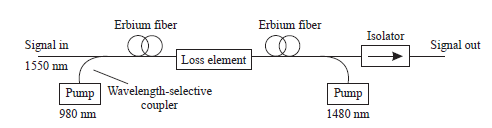
\includegraphics[width=338.3pt]{images/image124.png}
\end{center}
\end{frame}

\begin{frame}[shrink=20,t]{Ενισχυτές Raman}
\begin{itemize}
\item Η σκέδαση Raman είναι ένας ωραίος τρόπος να μεταφέρουμε ενέργεια από ένα laser άντλησης (pump) σε ένα σήμα.
\item Η φασματική απόσταση του pump και του σήματος καθορίζεται από το κέρδος Raman και είναι περίπου 100nm (\textasciitilde{}13THz).
\item Σε αντίθεση με τους EDFA μπορούν να ενισχύσουν το φως σε οποιοδήποτε μήκος κύματος αρκεί να υπάρχει κατάλληλο pump laser.
\item Έτσι μπορούμε να ενισχύσουμε το φως στην περιοχή των 1310nm αλλά και στην S-band (κάτω από τα 1528nm).
\item Πρόκειται για ένα κατανεμημένο σύστημα ενίσχυσης σε αντίθεση με τους ενισχυτές EDFA που παρέχουν τοπική μόνο ενίσχυση.
\item Επίσης με χρήση πολλών laser άντλησης μπορούμε να ενισχύσουμε διαφορετικά μήκη κύματος με διαφορετικό κέρδος.
\item Στα σύγχρονα συστήματα χρησιμοποιούμε ενισχυτές Raman για να έχουμε επιπλέον ενίσχυση σε συνδυασμό με EDFA.
\item Aπαιτούν laser άντλησης με ισχύ \textasciitilde{}1W…
\item O θόρυβος στους ενισχυτές Raman οφείλεται σε αστάθειες του laser άντλησης. Επίσης μπορεί να έχουμε και διαφωνία μεταξύ των WDM καναλιών
\end{itemize}
\end{frame}

\begin{frame}[shrink=20,t]{Η περίπτωση των ημιαγωγών}
\begin{itemize}
\item Στην περίπτωση αυτή, οι ενεργειακές καταστάσεις είναι πιο πολύπλοκες.
\item Για να συμβεί αυθόρμητη εκπομπή θα πρέπει ένα ηλεκτρόνιο το οποίο βρίσκεται στην ζώνη αγωγιμότητας (με ενέργεια \textit{Ε}$_{\text{2}}$) να επανασυνδεθεί με μία οπή που βρίσκεται στην ζώνη σθένους (με ενέργεια \textit{Ε}$_{\text{1}}$).
\item Η πυκνότητα πιθανότητας για να βρεθεί ένα ηλεκτρόνιο στη ζώνη αγωγιμότητας με ενέργεια \textit{Ε}$_{\text{2}}$ είναι \textit{f}$_{\text{\textit{c}}}$(\textit{E}$_{\text{2}}$)=\{1+exp[(\textit{E}$_{\text{2}}$-\textit{E}$_{\text{fc}}$)/\textit{k}$_{\text{B}}$/\textit{T}]\}$^{\text{-1}}$.
\item Η πυκνότητα πιθανότητας για να βρεθεί ένα ηλεκτρόνιο στη ζώνη σθένους με ενέργεια \textit{Ε}$_{\text{1}}$ είναι \textit{f}$_{\text{\textit{v}}}$(\textit{E}$_{\text{1}}$)=\{1+exp[(\textit{E}$_{\text{1}}$-\textit{E}$_{\text{fv}}$)/\textit{k}$_{\text{B}}$/\textit{T}]\}$^{\text{-1}}$.
\end{itemize}
\medskip
\begin{itemize}
\item Τα \textit{E}$_{\text{\textit{fc}}}$ και \textit{E}$_{\text{\textit{fv}}}$ ονομάζονται στάθμες Fermi.
\item O συνολικός ρυθμός αυθόρμητης εκπομπής φωτονίων με συχνότητα \textit{f} βρίσκεται αν αθροίσουμε όλες τις δυνατές μεταβάσεις με \textit{Ε}$_{\text{2}}$-\textit{Ε}$_{\text{1}}$=\textit{hf}.
\end{itemize}
\medskip
\begin{itemize}
\item Στις παραπάνω εξισώσεις Eg είναι η ελάχιστη τιμή που μπορεί να λάβει το Ε2-Ε1, ρcv είναι αριθμός των διαφορετικών διαθέσιμων καταστάσεων ανά μονάδα όγκου σε μία συχνότητα, \textit{m}$_{\text{\textit{r}}}$=\textit{m}$_{\text{\textit{c}}}$\textit{m}$_{\text{\textit{v}}}$/(\textit{m}$_{\text{\textit{c}}}$+\textit{m}$_{\text{\textit{v}}}$) όπου mc και mv είναι η μάζα των ηλεκτρονίων και των οπών
\end{itemize}
\begin{center}
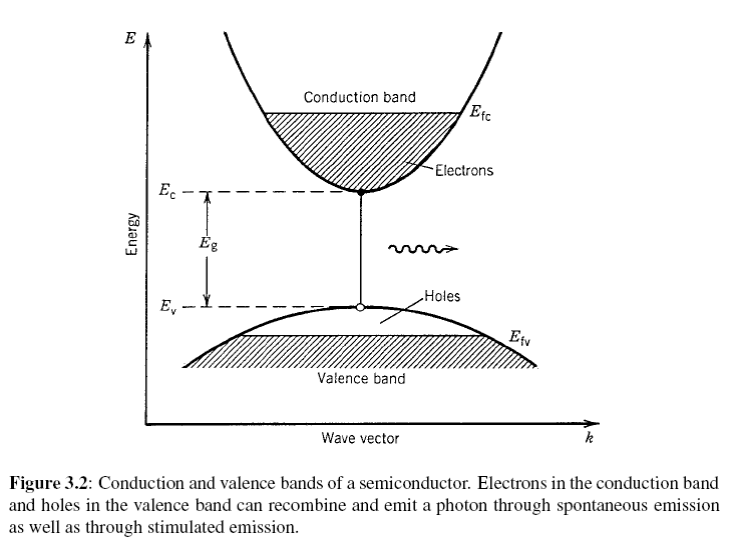
\includegraphics[width=199.4pt]{images/image127.png}
\end{center}
\begin{center}
$\displaystyle R_{\mathrm{spon}}(f)=\int\limits_{E_{c}}^{\infty}A(E_{1},E_{2})f_{c}(E_{2})\left[1-f_{v}(E_{1})\right]\rho_{cv}\,dE_{2}$ $\displaystyle \rho_{cv}=4\pi\frac{(2m_{r})^{3/2}}{h^{3}}(hf-E_{g})^{1/2}$\\[0.6ex]
\end{center}
\end{frame}

\begin{frame}[shrink=20,t]{Η περίπτωση των ημιαγωγών}
\begin{itemize}
\item Για να έχουμε \textit{R}$_{\text{stim}}$>\textit{R}$_{\text{abs}}$ θα πρέπει \textit{f}$_{\text{\textit{c}}}$(\textit{E}$_{\text{2}}$)>\textit{f}$_{\text{\textit{v}}}$(\textit{E}$_{\text{1}}$) ή \textit{Ε}$_{\text{\textit{fc}}}$-\textit{E}$_{\text{\textit{fv}}}$>\textit{E}$_{\text{2}}$-\textit{E}$_{\text{1}}$>\textit{E}$_{\text{\textit{g}}}$.
\item Επομένως για να υπερισχύει η εξαναγκασμένη εκπομπή θα πρέπει η διαφορά μεταξύ των δύο επιπέδων Fermi να είναι μεγαλύτερη από το \textit{E}$_{\text{\textit{g}}}$.
\item Στη θερμική ισορροπία έχουμε \textit{E}$_{\text{\textit{fc}}}$=\textit{E}$_{\text{\textit{fv}}}$ και επομένως η εξαναγκασμένη εκπομπή… δεν επιβιώνει.
\item Χρησιμοποιώντας ωστόσο επαφές pn και εξωτερική τάση μπορούμε να ικανοποιήσουμε την συνθήκη για να επικρατήσει η εξαναγκασμένη εκπομπή.
\end{itemize}
\medskip
\begin{itemize}
\item Πιθανότητα να βρεθεί ηλεκτρόνιο με ενέργεια Ε$_{\text{1}}$
\end{itemize}
\medskip
\begin{itemize}
\item Πιθανότητα να μην υπάρχει ηλεκτρόνιο με ενέργεια Ε$_{\text{1}}$ (δηλαδή να υπάρχει οπή!)
\end{itemize}
\begin{center}
$\displaystyle R_{\mathrm{spon}}(f)=\int\limits_{E_{c}}^{\infty}A(E_{1},E_{2})f_{c}(E_{2})\left[1-f_{v}(E_{1})\right]\rho_{cv}\,dE_{2}$\\[0.6ex]
$\displaystyle R_{\mathrm{stim}}(f)=\int\limits_{E_{c}}^{\infty}B(E_{1},E_{2})f_{c}(E_{2})\left[1-f_{v}(E_{1})\right]\rho_{cv}\,\rho\,dE_{2}$\\[0.6ex]
$\displaystyle R_{\mathrm{abs}}(f)=\int\limits_{E_{c}}^{\infty}B(E_{1},E_{2})f_{v}(E_{1})\left[1-f_{c}(E_{2})\right]\rho_{cv}\,\rho\,dE_{2}$\\[0.6ex]
\end{center}
\end{frame}

\begin{frame}[shrink=20,t]{Η περίπτωση της επαφής pn}
\begin{itemize}
\item Οι επαφές pn σχηματίζονται από συνένωση (ημιαγωγικών) υλικών με διαφορετικών ειδών προσμίξεις
\begin{itemize}
\item τύπου-p: οι προσμίξεις δημιουργούν πολλές οπές στην ζώνη σθένους
\item τύπου-n: πολλά ηλεκτρόνια στην ζώνη αγωγιμότητας.
\end{itemize}
\item Χωρίς εξωτερική διέγερση η στάθμη Fermi πρέπει να είναι κοινή κατά μήκος του υλικού.
\item Όταν έρχονται σε επαφή τα δύο υλικά, οπές από το p κινούνται προς το n και ηλεκτρόνια από το n κινούνται προς το p.
\item Mε τον τρόπο αυτό δημιουργείται ένα έλλειμμα θετικού φορτίου (δλδ αρνητικό φορτίο) στην περιοχή p και θετικό φορτίο στην περιοχή n που απαγορεύει την περαιτέρω κίνηση φορέων εξαιτίας της ανάπτυξης διαφοράς δυναμικού.
\item Όταν όμως εφαρμόζουμε τάση θετική (ορθή) τάση, τότε το δυναμικό μειώνεται.
\item Επίσης οι στάθμες Fermi απομακρύνονται και υπάρχει μία περιοχή κοντά στην επαφή όπου υπάρχουνε  και οπές και ηλεκτρόνια τα οποία μπορούνε να συνδυαστούν και μέσω αυθόρμητης ή \textbf{εξαναγκασμένης} εκπομπής να παράγουνε φωτόνια
\end{itemize}
\begin{center}
\setlength{\unitlength}{0.000094pt}
\begin{picture}(3428992,1592855)
\put(0,0){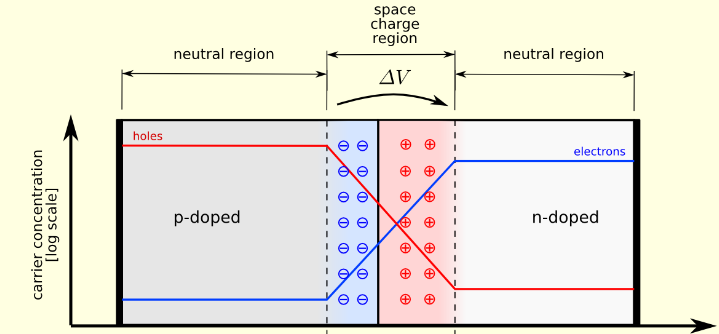
\includegraphics[width=322.9pt]{images/image132.png}}
\put(1190317,0){\footnotesize \shortstack{Χωρίς τάση στα άκρα της}}
\put(941251,0){\footnotesize \shortstack{Με ορθή πόλωση (θετική τάση)}}
\end{picture}
\end{center}
\end{frame}

\begin{frame}[shrink=10,t]{Ενισχυτής ημιαγωγού (semiconductor optical amplifier –SOA).}
\begin{itemize}
\item προϋπάρχουν των EDFAs αλλά δεν είναι εξίσου καλοί.
\item Βρίσκουν εφαρμογές ως μεταγωγείς (switches) ή μετατροπείς μήκος κύματος.
\item Στην ουσία πρόκειται για μία επαφή pn όπου όμως έχει δοθεί ιδιαίτερη σημασία στο να μην λαμβάνουν χώρα ανακλάσεις στα άκρα της διάταξης.
\item Στην πράξη δεν χρησιμοποιείται μία απλή επαφή αλλά μία ετεροέπαφη (heterostructure).
\item Οι SOAs έχουν μεγαλύτερο εύρος ζώνης (100nm) από τους EDFA αλλά:
\begin{itemize}
\item εισάγουν διαφωνία μεταξύ των καναλιών.
\item Η σύζευξη με την ίνα θέλει προσοχή.
\item Το κέρδος και η ισχύς εξόδου είναι μικρότερες των EDFA.
\item υπάρχει υψηλότερη απώλεια λόγω πόλωσης.
\item εισάγουν περισσότερο θόρυβο.
\item είναι δύσκολο να επιτύχουμε τις μικρές ανακλαστικότητες που απαιτούνται (10$^{-4}$).
\end{itemize}
\end{itemize}
\end{frame}

\begin{frame}[shrink=10,t]{Οπτικοί Πομποί - Απαιτήσεις}
\begin{itemize}
\item Στην περίπτωση των συστημάτων WDM χρειάζεται ο οπτικός πομπός να έχει τα εξής χαρακτηριστικά:
\begin{itemize}
\item υψηλή ισχύ εκπομπής (τυπικές τιμές για laser είναι 0-10dBm) με μικρό κατώφλι ρεύματος και καλή απόδοση (=οπτική ισχύς προς ρεύμα οδήγησης)
\item μικρό φασματικό εύρος ώστε το σήμα να έχει όσο το δυνατόν μικρότερο εύρος ζώνης
\item σταθερότητα μήκους κύματος εκπομπής
\end{itemize}
\item Στην περίπτωση πηγών άντλησης χρειαζόμαστε:
\begin{itemize}
\item ισχύ εκπομπής 100-200mW για τους ενισχυτές EDFA
\item μερικά W για τους ενισχυτές Raman
\end{itemize}
\end{itemize}
\end{frame}

\begin{frame}[shrink=10,t]{Πηγές laser}
\begin{itemize}
\item Πρόκειται για ενισχυτές που τοποθετούνται εντός ενός οπτικού αντηχείου (οπτική κοιλότητα) και μέσω της ανάδρασης αρχίζουν να ταλαντώνονται.
\begin{itemize}
\item Ημιαγωγικά laser όπου το οπτικό κέρδος παρέχεται από ημιαγωγούς
\item Laser ίνας όπου χρησιμοποιείται ίνα ντοπαρισμένη με έρβιο για να παρέχει το οπτικό κέρδος.
\end{itemize}
\item Τα ημιαγωγικά laser είναι ιδιαίτερα δημοφιλή καθώς:
\begin{itemize}
\item έχουν μικρές διαστάσεις (\textasciitilde{}100μm).
\item δεν απαιτούν οπτική άντληση.
\item πρόκειται για επαφές pn οπότε κατασκευάζονται εύκολα.
\item είναι αρκετά αποδοτικά
\end{itemize}
\item Η κύρια εφαρμογή των fiber laser είναι για την γέννηση περιοδικών παλμών με πολύ μικρό εύρος
\end{itemize}
\end{frame}

\begin{frame}[shrink=20,t]{Laser – αρχή λειτουργίας}
\begin{itemize}
\item Υποθέτουμε πως ένα υλικό με οπτικό κέρδος τοποθετείται μέσα σε μία κοιλότητα Fabry-Perot.
\item Αυτό έχει ως αποτέλεσμα να έχουμε υψηλό κέρδος μόνο στα μήκη κύματος συντονισμού της κοιλότητας FP.
\item H λογική είναι ίδια με την ανάλυση του φίλτρου FP. Σε κάθε διέλευση τα κύματα που συμβάλλουν θετικά ενισχύονται. Τα κύματα αυτά αντιστοιχούν σε μήκη κύματος συντονισμού.
\item Τα αρχικά κύματα γεννιούνται εξαιτίας αυθόρμητης εκπομπής.
\item Η εξαναγκασμένη εκπομπής ενισχύει το αρχικό φως και τελικά υπερισχύει της αυθόρμητης η οποία καταστέλλεται.
\item Για να συμβεί αυτό, το ηλεκτρικό ρεύμα που παρέχουμε στο μέσο ενίσχυσης (επαφή pn) πρέπει να ξεπεράσει μία τιμή κατωφλίου.
\item Κάτω από το κατώφλι αυτό, η διάταξη απλά δρα ως ενισχυτής (στα μήκη κύματος συντονισμού).
\end{itemize}
\begin{center}
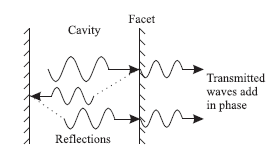
\includegraphics[width=262.0pt]{images/image133.png}
\end{center}
\end{frame}

\begin{frame}[shrink=10,t]{Έναρξη των ταλαντώσεων}
\begin{itemize}
\item Δύο συνθήκες θα πρέπει να ισχύουν ώστε το laser να αρχίσει να ταλαντώνεται σε ένα δεδομένο μήκος κύματος:
\begin{itemize}
\item Το μήκος κύματος να είναι εντός της φασματικής περιοχής που έχουμε οπτικό κέρδος.
\item Το μήκος κύματος να είναι κοντά στο μήκος κύματος συντονισμού της κοιλότητας.
\end{itemize}
\item Η παραπάνω συνθήκες ενδεχομένως να πληρούνται για περισσότερα του ενός μήκη κύματος.
\item Επομένως το laser θα εκπέμπει πολλά μήκη κύματος ή όπως αναφέρεται στην βιβλιογραφία, “θα υποστηρίζει πολλούς τρόπους”.
\item Στην περίπτωση αυτή ονομάζουμε το laser πολλαπλών τρόπων (multimode).
\item Για τηλεπικοινωνιακές εφαρμογές θα θέλαμε το laser να είναι singlemode.
\end{itemize}
\end{frame}

\begin{frame}[shrink=20,t]{Φάσματα Εκπομπής}
\begin{itemize}
\item Στην πράξη όλα τα laser είναι πολύτροπα αλλά σε ορισμένα το πλάτος ενός τρόπου είναι πολύ μεγάλο σε σχέση με τους άλλους.
\item Single mode laser έχουμε όταν το πλάτος των πλευρικών τρόπων είναι \ensuremath{\ge}30dB κάτω από το πλάτος του κύριου τρόπου.
\item Για να επιτύχουμε single mode λειτουργία μπορούμε να χρησιμοποιήσουμε έναν επιπλέον μηχανισμό συντονισμού.
\end{itemize}
\begin{center}
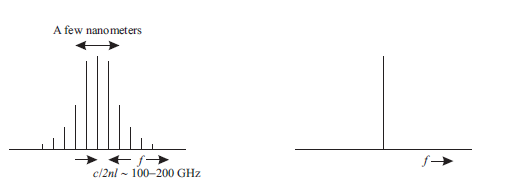
\includegraphics[width=338.3pt]{images/image134.png}
\end{center}
\end{frame}

\begin{frame}[shrink=20,t]{Laser κατανεμημένης ανάδρασης}
\begin{itemize}
\item Στην περίπτωση των laser Fabry Perot η ανάδραση λαμβάνει χώρα στις ακριανές επιφάνειες – \textit{τοπική ανάδραση}
\item Μπορούμε ωστόσο να υποβοηθήσουμε την ανάδραση κατανεμημένα αν τοποθετήσουμε ανακλαστήρες κατά μήκος της κοιλότητας.
\end{itemize}
\begin{center}
\setlength{\unitlength}{0.000086pt}
\begin{picture}(4150208,1143008)
\put(0,0){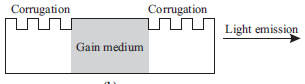
\includegraphics[width=358.2pt]{images/image136.png}}
\put(0,0){\footnotesize \shortstack{Distributed Feedback (DFB) laser}}
\put(596467,0){\footnotesize \shortstack{Distributed Bragg Reflector (DBR) laser}}
\end{picture}
\end{center}
\end{frame}

\begin{frame}[shrink=20,t]{DBR και DFB}
\begin{itemize}
\item Και στις δύο περιπτώσεις (DFB+DBR) το μήκος κύματος που προκύπτει από την συνθήκη Bragg είναι ο κύριος τρόπος και οι υπόλοιποι τρόποι του laser καταστέλλονται.
\item Στην περίπτωση του DBR η ανάδραση βρίσκεται εκτός της ενεργού περιοχής και επομένως είναι δυνατόν να ελέγξουμε πιο αποδοτικά
\item Για παράδειγμα αλλάζοντας το δείκτη διάθλασης του φράγματος Bragg μπορούμε να αλλάξουμε το μήκος κύματος εκπομπής (συντονισμός).
\item Τα laser αυτά χρειάζονται έναν απομόνωση ο οποίος απαγορεύει σε ακτινοβολία από το υπόλοιπο σύστημα να γυρίσει στο laser και να μεταβάλει την ισχύ εκπομπής και το μήκος κύματος.
\item Επίσης χρειάζεται και ένα μηχανισμό ψυξης (thermoelectric cooler) ο οποίος έχει ως σκοπό την διατήρηση των χαρακτηριστικών του laser σταθερά.
\item Μπορούμε να έχουμε πολλά laser σε ένα chip – πηγές WDM. Ωστόσο αυτό δεν συναντάται πολύ συχνά στην πράξη.
\end{itemize}
\end{frame}

\begin{frame}[shrink=20,t]{Laser εξωτερικής κοιλότητας}
\begin{itemize}
\item Η καταστολή των τρόπων του laser μπορεί να λάβει χώρα και με μία δεύτερη κοιλότητα.
\item Με τον τρόπο αυτό επιβιώνουνε μόνο τα μήκη κύματος που υποστηρίζονται και στις δύο κοιλότητες.
\item Αντί μίας κοιλότητας FB μπορούμε να χρησιμοποιήσουμε ένα περιστρεφόμενο φράγμα. Στην περίπτωση αυτή τοποθετούμε μία αντιανακλαστική επίστρωση στην μία άκρη της ενεργού περιοχής.
\item Περιστρέφοντας το φράγμα πετυχαίνουμε συντονισμό (αλλαγή μήκους κύματος εκπομπής).
\item Μπορούμε να χρησιμοποιήσουμε και άλλου είδους εξωτερικά φίλτρα.
\item Τα laser εξωτερικής κοιλότητας χρησιμοποιούνται κυρίως σε εφαρμογές οπτικών οργάνων μέτρησης και όχι σε καθαρά τηλεπικοινωνιακά συστήματα λόγω του υψηλότερου κόστους.
\item Δεν διαμορφώνονται τόσο εύκολα όσο τα DFB (μεγάλο μήκος κοιλότητας).
\end{itemize}
\begin{center}
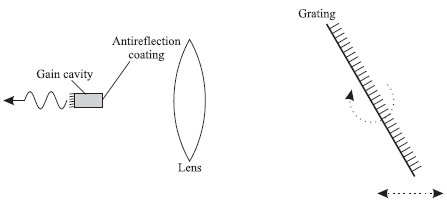
\includegraphics[width=170.3pt]{images/image137.png} 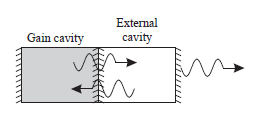
\includegraphics[width=168.0pt]{images/image138.png}
\end{center}
\end{frame}

\begin{frame}[shrink=20,t]{VCSELs}
\begin{itemize}
\item Οι τρόποι σε μία κοιλότητα FB απέχουν συχνοτικά κατά FSR=1/2/\textit{τ}\textit{=c/}(2\textit{nl}) όπου \textit{l} το μήκος της κοιλότητας.
\item Άρα αν είχαμε αρκετά μικρή κοιλότητα (μικρό \textit{l}) τότε οι τρόποι του laser θα ήτανε μεγάλο και επομένως θα είχαμε μόνο ένα μήκος κύματος μέσα στο εύρος ζώνης οπτικής ενίσχυσης.
\item Είναι πολύ πιο εύκολο αν η κοιλότητα “γραφτεί” κάθετα στο υπόστρωμα του ολοκληρωμένου.
\item Αυτά τα laser ονομάζονται για αυτό το λόγω vertical cavity surface emitting lasers (VCSELs).
\item Ωστόσο χρειάζονται καλής ποιότητας καθρέφτες στις άκρες για να λάβει αρχίσουνε οι ταλαντώσεις (εξαιτίας της μικρής ενεργού περιοχής έχουμε μικρό κέρδος).
\item Συνήθως αυτό επιτυγχάνεται με ένα sandwich από διηλεκτρικά υλικά τα οποία δρουν ως (επιλεκτικοί ως προς το μήκος κύματος βέβαια) καθρέφτες.
\end{itemize}
\begin{center}
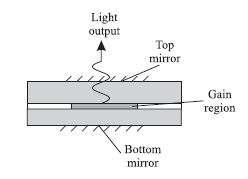
\includegraphics[width=207.8pt]{images/image139.png}
\end{center}
\end{frame}

\begin{frame}[shrink=20,t]{VCSELs στην πράξη:}
\begin{itemize}
\item Προβλήματα
\begin{itemize}
\item Αρκετά μεγάλη αντίσταση εισόδου για το ρεύμα έγχυσης\ensuremath{\Rightarrow}ανάγκη για καλό θερμοκρασιακό έλεγχο
\item Ενώ τα VCSELs ήτανε γνωστά από το 1979 για αυτό το λόγω δεν υλοποιηθήκανε πριν το 2000.
\end{itemize}
\item Πλεονεκτήματα:
\begin{itemize}
\item πιο εύκολη σύζευξη με ίνα
\item πιο εύκολο packaging
\item ολοκλήρωση σε συστάδες (arrays)
\item 1.3μm και 0.85μm VCSELs υπάρχουν ήδη εμπορικά διαθέσιμα.
\end{itemize}
\end{itemize}
\medskip
\begin{itemize}
\item VCSELs σε συστάδες: ιδανική λύση για WDM
\item Όλες οι πηγές των καναλιών σε ένα chip!
\item Εναλλακτικά έχουμε φτιάξει ένα πολύ καλό tunable laser!
\item Ωστόσο δεν υπάρχει εύκολος τρόπος (ακόμα) να συζεύξουμε αποδοτικά όλα τα μήκη κύματος στην ίνα.
\item Επίσης αν δεν λειτουργεί ένα laser… πετάμε όλο το chip!
\end{itemize}
\begin{center}
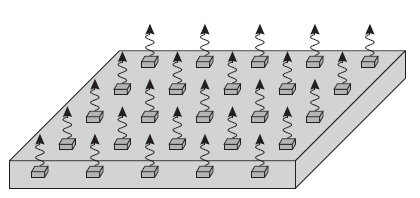
\includegraphics[width=318.2pt]{images/image140.png}
\end{center}
\end{frame}

\begin{frame}[shrink=10,t]{LEDs: Light Emitting Diodes}
\begin{itemize}
\item Τα laser ενδεχομένως να είναι αρκετά ακριβοί πομποί στην περίπτωση όπου οι ρυθμοί μετάδοσης είναι χαμηλοί και οι αποστάσεις μικρές.
\item Στην περίπτωση αυτή μπορούμε να χρησιμοποιήσουμε LEDs.
\item Στην ουσία οι LEDs είναι επαφές pn όπως και τα LASER χωρίς όμως καθρέφτες στα άκρα τους.
\item Εδώ δεν έχουμε εξαναγκασμένη εκπομπή αλλά αυθόρμητη εκπομπή.
\item Το φάσμα εκπομπής είναι πολύ μεγάλο ενώ η ισχύς εκπομπής δεν ξεπερνά εύκολα τα -20dBm.
\item Μπορούν να χρησιμοποιηθούν για μετάδοση δεδομένων με ρυθμούς μερικών εκατοντάδων Mb/s.
\end{itemize}
\end{frame}

\begin{frame}[shrink=20,t]{Συντονισμός των πηγών laser}
\begin{itemize}
\item Ο συντονισμός είναι μια ιδιαίτερη επιθυμητή ιδιότητα ειδικά σε συστήματα WDM.
\item Ωστόσο δεν επιτυγχάνεται και τόσο εύκολα. Μερικοί τρόποι συντονισμού:
\begin{itemize}
\item ηλεκτρονικός: όταν ένα ηλεκτρικό ρεύμα διαρρέει έναν ημιαγωγό αλλάζει το δείκτη διάθλασης (n) κατά 0.5\%-2\% και επιφέρει μία ανάλογε μεταβολή στο μήκος κύματος εκπομπής (10-15nm στα 1.55μm)
\item θερμικός: Το μήκος κύματος αλλάζει κατά 0.1nm/$^{\text{o}}$C. Ωστόσο δεν είναι καλή ιδέα, τα θερμά laser καταπονούνται.
\item μηχανικός (με εξωτερική κοιλότητα): συνήθως έχουνε ως αποτέλεσμα ογκώδεις διατάξεις.
\end{itemize}
\item Ιδανικά θα θέλαμε δυνατότητα συντονισμού 100nm και σταθερότητα στη λειτουργία.
\item Οι μέθοδοι συντονισμού υπάρχουνε εδώ και πολλά χρόνια αλλά μόλις τώρα εμφανίζονται στο εμπόριο συντονιζόμενες πηγές (λόγω της πολυπλοκότητας κατασκευής και ελέγχου του συντονισμού).
\end{itemize}
\end{frame}

\begin{frame}[shrink=10,t]{Διαμόρφωση των οπτικών πηγών.}
\begin{itemize}
\item Δεν αρκεί μία πηγή απλά να παράγει φως. Θα πρέπει αυτό το φως να διαμορφώνεται κατάλληλα ώστε να μεταφέρει πληροφορία.
\item Ο πιο απλός (και συχνός στις οπτικές επικοινωνίες τρόπος) είναι το on-off keying (ΟΟΚ) το οποίο θα το δούμε και παρακάτω.
\begin{itemize}
\item “0” αντιστοιχεί σε μη εκπομπή φωτός (πηγή σβηστή)
\item “1” αντιστοιχεί σε εκπομπή φωτός (παλμός, πηγή αναμμένη).
\end{itemize}
\item Πως αναβοσβήνουμε επομένως τις πηγές μας;
\begin{itemize}
\item \textit{άμεσα}: απλά στέλνουμε ή δεν στέλνουμε ρεύμα στο laser. Χωρίς ρεύμα το laser δεν παράγει φωτόνια και “σβήνει”.
\item \textit{εξωτερικά}: χρησιμοποιούμε κάποιο άλλο στοιχείο \textbf{εξωτερικά} του laser για να συνθέσουμε τους παλμούς μας.
\end{itemize}
\end{itemize}
\end{frame}

\begin{frame}[shrink=10,t]{Άμεση διαμόρφωση}
\begin{center}
\setlength{\unitlength}{0.000066pt}
\begin{picture}(3286125,2752725)
\put(0,0){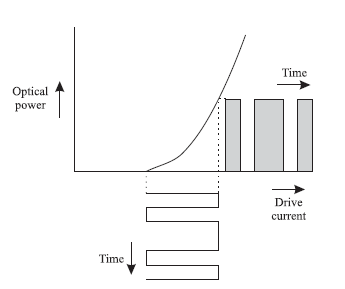
\includegraphics[width=217.3pt]{images/image141.png}}
\end{picture}
\end{center}
\centering\footnotesize Αρκετά φθηνή μέθοδος για την επίτευξη διαμόρφωσης σε ένα ημιαγωγικό laser δεν μπορεί να χρησιμοποιηθεί σε fiber laser (εξαιτίας του μεγάλου χρόνου απόκρισης των κβαντικών μεταβάσεων)\par
\end{frame}

\begin{frame}[shrink=10,t]{Απόκριση laser σε άμεση διαμόρφωση}
\begin{center}
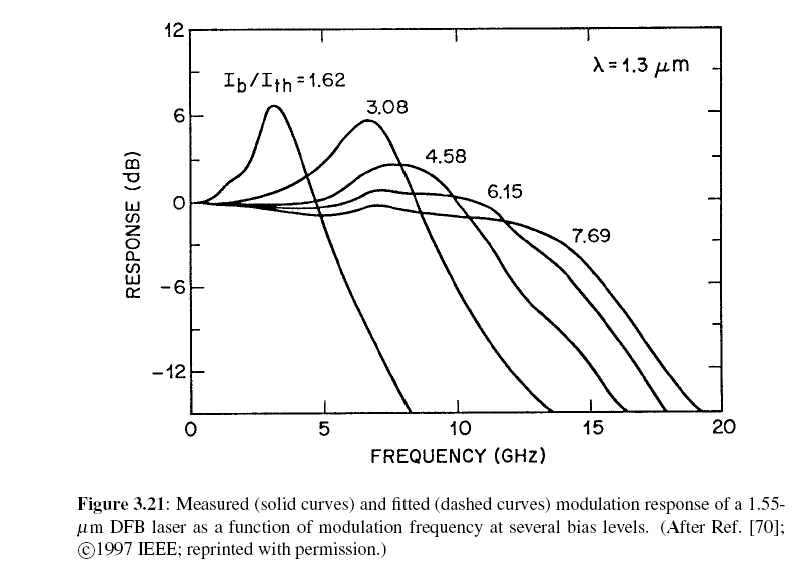
\includegraphics[width=274.7pt]{images/image142.png}
\end{center}
\end{frame}

\begin{frame}[shrink=10,t]{Έμμεση διαμόρφωση}
\begin{itemize}
\item Το να ανοιγοκλείνει κανείς το laser δεν είναι πάντα καλή ιδέα.
\item Εισάγεται chirp\ensuremath{\Rightarrow}αυξάνει το εύρος ζώνης του σήματος.
\item Θα μπορούσε κανείς βέβαια να μην σβήνει τελείως το laser και να μεταδίδει μικρή ισχύ στο “0”.
\item Ωστόσο αυτό σημαίνει πως μειώνεται ο λόγος σβέσης = \textit{P}$_{\text{“1”}}$/\textit{P}$_{\text{“0”}}$ (\textasciitilde{}7dB).
\item Το σύστημα έτσι γίνεται πιο ευαίσθητο στο θόρυβο.
\item Επομένως σε συστήματα με υψηλό ρυθμό μετάδοσης χρησιμοποιούμε την εξωτερική διαμόρφωση.
\item Δύο είδη εξωτερικών διαμορφωτών χρησιμοποιούνται στην πράξη:
\begin{itemize}
\item διαμορφωτές βασισμένοι σε LiNbO$_{\text{3}}$ (νιοβικό λίθιο).
\item διαμορφωτές ηλεκτρο- απορρόφησης  (electroabsorption –EA).
\end{itemize}
\end{itemize}
\end{frame}

\begin{frame}[shrink=20,t]{Διαμορφωτής MZI}
\begin{itemize}
\item Το LiNbO3 επιτρέπει να ελέγξουμε τη διαφορά δρόμου στο ΜΖΙ χρησιμοποιώντας τάση.
\item Για μηδενική τάση τα δύο άκρα του MZI έχουν μηδενική διαφορά δρόμου (θετική συμβολή φως “περνάει”).
\item Για τάση V=Vπ σχηματίζεται διαφορά φάσης π (καταστροφική συμβολή φως “δεν περνάει”)
\item Γενικά πετυχαίνουμε καλούς λόγους σβέσης (15-20dB) και καλό έλεγχο του chirp
\item Ωστόσο χρειάζεται έλεγχο της πόλωσης επειδή η διάταξη είναι ευαίσθητη στην πόλωση.
\end{itemize}
\begin{center}
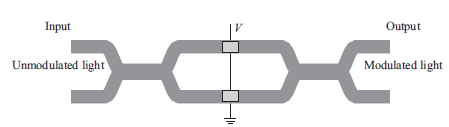
\includegraphics[width=233.5pt]{images/image143.png} 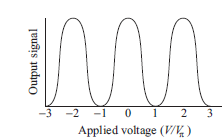
\includegraphics[width=104.8pt]{images/image144.png}
\end{center}
\end{frame}

\begin{frame}[shrink=10,t]{Ηλεκτρόαποροφηση (Electroabsorption)}
\begin{itemize}
\item Αποτελούν μία χαμηλού κόστους εναλλακτική στους διαμορφωτές LiNbO$_{\text{3}}$
\item Στην ουσία βασίζονται στο γεγονός ότι σε ορισμένα υλικά η απαγορευμένη περιοχή όπου λαμβάνει χώρα η απορρόφηση του φωτός (δείτε τα περί ημιαγωγών).
\item Με την εφαρμογή ηλεκτρικού πεδίου η περιοχή αυτή μικραίνει και επομένως μπορεί να αποροφήσει φωτόνια.
\item Το φαινόμενο αυτό ονομάζεται Franz-Keldysh.
\item Οι διαμορφωτές ΕΑ μπορούν να χρησιμοποιηθούνε για ρυθμούς 2.5Gb/s-10Gb/s αλλά δεν είναι τόσο καλοί όσο οι ΜΖΙ.
\item Μπορούν να συνδυαστούν στο ίδιο chip με την δίοδο laser.
\end{itemize}
\end{frame}

\begin{frame}[shrink=20,t]{Οπτικοί Δέκτες}
\begin{itemize}
\item Μετατρέπουν το οπτικό σήμα σε ηλεκτρικό ρεύμα.
\item Στοιχεία ενός δέκτη:
\begin{itemize}
\item οπτικός προενισχυτής: ενισχύει το σήμα πριν την φώραση.
\item Φωτοδέκτης: μετατρέπει το ρεύμα φωτονίων σε ρεύμα ηλεκτρονίων (φως\ensuremath{\Rightarrow}ηλεκτρικό ρεύμα).
\item Ηλεκτρονικός ενισχυτής: ενισχύει το ηλεκτρικό ρεύμα
\item Κύκλωμα απόφασης. Αποφασίζει για το σύμβολο που μεταδόθηκε.
\end{itemize}
\end{itemize}
\begin{center}
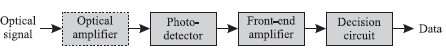
\includegraphics[width=338.3pt]{images/image145.png}
\end{center}
\end{frame}

\begin{frame}[shrink=20,t]{Φωτοδέκτης}
\begin{itemize}
\item Αποτελούνται από ημιαγωγικά υλικά
\item Τα φωτόνια απορροφούνται από το υλικό και μετατρέπονται σε ηλεκτρικό ρεύμα.
\item Στην ουσία τα ηλεκτρόνια της ζώνης σθένους απορροφώντας φωτόνια μεταφέρονται στη ζώνη αγωγιμότητας.
\item Τα ηλεκτρόνια αυτά αφήνουν πίσω τους μία οπή στην ζώνη σθένους.
\item Με την εφαρμογή ηλεκτρικού πεδίου, τα ζεύγη αυτά δημιουργούν ηλεκτρικό ρεύμα.
\item Θα πρέπει βέβαια \textit{hf}>\textit{E}$_{\text{\textit{g}}}$, δηλαδή υπάρχει μία συχνότητα κάτω από την οποία το υλικό δεν απορροφά.
\end{itemize}
\begin{center}
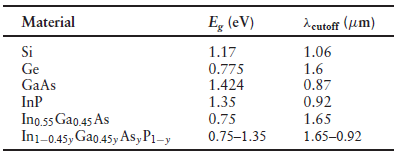
\includegraphics[width=207.9pt]{images/image146.png} 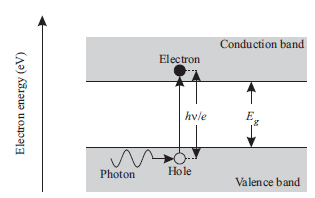
\includegraphics[width=130.4pt]{images/image147.png}
\end{center}
\end{frame}

\begin{frame}[shrink=20,t]{Η απορρόφηση είναι καλό πράγμα…}
\begin{itemize}
\item Πόσα φωτόνια όμως απορροφούνται; Αυτό εξαρτάται από το συντελεστή απορρόφησης \textit{a }του υλικού.
\item \textit{P}$_{\text{out}}$=\textit{P}$_{\text{in}}$exp(-\textit{aL}) επομένως η ισχύς που απορροφάται είναι \textit{P}$_{\text{abs}}$=\textit{P}$_{\text{in}}$-\textit{P}$_{\text{out}}$=(1-exp(-\textit{aL}))\textit{P}$_{\text{in}}$.
\item H απόδοση η του φωτοδέκτη είναι \textit{η}=\textit{P}$_{\text{abs}}$/\textit{P}$_{\text{in}}$=1-exp(-\textit{aL}).
\item Τυπικές τιμές για το \textit{a} είναι 10$^{4}$/cm και επομένως με μήκος \textit{L}=10μm.
\item Αποκρισημότητα \textit{R} ορίζεται ως \textit{R}=\textit{Ι}$_{\text{p}}$/\textit{P}$_{\text{in}}$ όπου \textit{I}$_{\text{p}}$ το φωτόρευμα.
\item Είναι εύκολο να δούμε ότι \textit{R}=\textit{εη}/(\textit{hf})=\textit{εηλ}/(\textit{hc})=\textit{ηλ}/1.24 (A/W) όπου το \textit{λ} μετριέται σε μm.
\item Ωστόσο σε έναν ομογενή ημιαγωγό είναι δύσκολο να πετύχουμε μεγάλο η επειδή τα ηλεκτρόνια επανασυνδέονται με τις οπές.
\item Για το λόγο αυτό χρησιμοποιούμε μία επαφή pn όπου εφαρμόζουμε (σχετικά μεγάλη) ανάστροφη τάση και επομένως τα ζεύγη οπών ηλεκτρονίων φτάνουνε γρήγορα στο εξωτερικό κύκλωμα.
\item Το πεδίο είναι ιδιαίτερα ισχυρό στην επαφή των δύο υλικών pn.
\item Ωστόσο μακριά από την επαφή, δημιουργείται ένα ρεύμα διάχυσης το οποίο δεν μπορεί να ανταποκριθεί γρήγορα στις αλλαγές της οπτικής ισχύος και επομένως επιβαρύνει άσκοπα την φασματική απόκριση της φωτοδιόδου.
\end{itemize}
\end{frame}

\begin{frame}[shrink=10,t]{Δημιουργία Φωτορεύματος στην επαφή pn}
\begin{center}
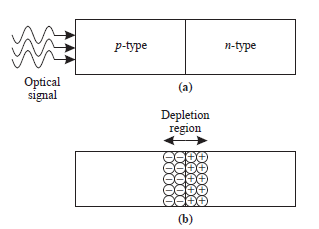
\includegraphics[width=193.1pt]{images/image148.png} 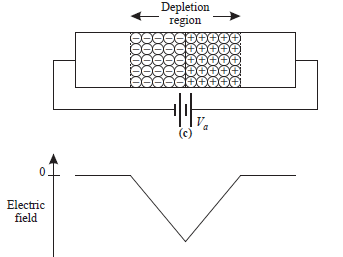
\includegraphics[width=185.0pt]{images/image149.png}
\end{center}
\end{frame}

\begin{frame}[shrink=20,t]{Φωτοδίοδοι pin}
\begin{itemize}
\item Μπορούμε να βελτιώσουμε και άλλο την απόδοση αν χρησιμοποιήσουμε ένα στρώμα ανόθευτου (intrinsic) ημιαγωγού ανάμεσα στα στρώματα p και n.
\item Σε αυτή τη δομή η περιοχή απογύμνωσης εκτείνεται κατά μήκος και του ανόθευτου στρώματα.
\item Γενικά το μήκος των περιοχών \textit{p} και \textit{n} είναι πολύ μικρότερο της περιοχής \textit{i}\textit{ }και επομένως το μεγαλύτερο μέρος της απορρόφησης θα λάβει χώρα στο \textit{i}.
\item Μία καλύτερη τακτική είναι να χρησιμοποιήσουμε ένα υλικό στις περιοχές \textit{p} και \textit{n} που να είναι διαφανές (να μην απορροφά) στο μήκος κύματος που μας ενδιαφέρει.
\item Π.χ. InP είναι διαφανές για λ>0.92μm ενώ για το InGaAs αυτό  συμβαίνει για λ>1.65μm.
\item Με τέτοιες δομές αποφεύγεται και το ρεύμα διάχυσης που είδαμε στις επαφές pn.
\end{itemize}
\begin{center}
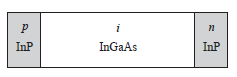
\includegraphics[width=338.3pt]{images/image150.png}
\end{center}
\end{frame}

\begin{frame}[shrink=10,t]{Φωτοδίοδοι APD}
\begin{itemize}
\item Στις φωτοδιόδους pin υπάρχει μία βασική αρχή: ένα φωτόνιο παράγει (το πολύ) ένα ηλεκτρόνιο.
\item Ωστόσο υπάρχουνε φωτοδίοδοι που αψηφούν αυτό τον απλό κανόνα.
\item Σε αυτές τις φωτοδιόδους υπάρχει ένας μηχανισμός εσωτερικού ηλεκτρονικού κέρδους.
\item Ο μηχανισμός αυτός οφείλεται στο φαινόμενο της χιονοστοιβάδας (avalanche)
\item Υπό υψηλό ηλεκτρικό πεδίο, ένα ηλεκτρόνιο μπορεί να “κλωτσήσει” ένα ηλεκτρόνιο από την ζώνη σθένους στη ζώνη αγωγιμότητας.
\item Αυτό το ηλεκτρόνιο είναι πλέον φορέας του ηλεκτρικού ρεύματος και μπορεί εκ νέου να κλωτσήσει και άλλα ηλεκτρόνια με τον ίδιο τρόπο.
\item Η διαδικασία αυτή ονομάζεται πολλαπλασιασμός χιονοστοιβάδας (avalanche multiplication).
\item Οι δέκτες ονομάζονται avalanche photodiodes (ΑPD).
\end{itemize}
\end{frame}

\begin{frame}[t]{Οπτικοί μεταγωγείς (switches)}
\begin{itemize}
\item Υπάρχουν ορισμένες κρίσιμες λειτουργίες στις οποίες μπορούμε να χρησιμοποιήσουμε οπτικούς μεταγωγείς:
\begin{itemize}
\item Δημιουργία και υποστήριξη των lightpaths (provisioning): αποφυγή χειροκίνητων αλλαγών στο τρόπο διαρρύθμισης των οπτικών ινών.
\item Προστασία: δρομολόγηση της κίνησης σε μία δευτερεύουσα ίνα σε περίπτωση αστοχίας υλικού (protection switching).
\item Δρομολόγηση πακέτων (packet switching)
\item Εξωτερική διαμόρφωση.
\end{itemize}
\end{itemize}
\end{frame}

\begin{frame}[shrink=20,t]{Χαρακτηριστικά των switch}
\begin{itemize}
\item \textit{Χρόνος μεταγωγής} (χρόνος αλλαγής της κατάστασης του switch).
\item \textit{Αριθμός θυρών} εισόδου και εξόδου.
\item \textit{Λόγος σβέσης} (λόγος της ισχύος που ανιχνεύεται όταν το switch αφήνει να περάσει το σήμα προς την ισχύ που ανιχνεύεται όταν αυτό δεν περνάει).
\item \textit{Απώλειες εισαγωγής} (επιπλέον απώλειες που εισάγονται από το δομικό στοιχείο. Είναι ίδιες για κάθε θύρα του?).
\item \textit{Επίπεδο διαφωνίας} (πόση ανεπιθύμητη ισχύ ανιχνεύεται στην έξοδο του switch).
\item \textit{Ευαισθησία στην πόλωση }(απώλειες που εξαρτώνται από την πόλωση).
\item \textit{Latching}: το switch μπορεί να διατηρεί την κατάσταση του ακόμα και όταν δεν τροφοδοτείται με ρεύμα.
\item Εξακρίβωση κατάστασης του switch (για να επιβεβαιώνετε η ορθή λειτουργία του δικτύου).
\item Αντοχή – μεγάλος χρόνος λειτουργίας χωρίς σφάλματα.
\end{itemize}
\end{frame}

\begin{frame}[shrink=20,t]{Φτιάχνοντας μεγάλα switch}
\begin{itemize}
\item Αριθμός μεταγωγικών στοιχείων (switching elements) που πρέπει να συνδυαστούν. Μας ενδιαφέρει το κόστος των στοιχείων που εξαρτάται από:
\begin{itemize}
\item το πλήθος των στοιχείων τους
\item τη δυνατότητα εύκολης συσκευασίας (packaging)
\item την ευκολία κατασκευής των στοιχείων
\end{itemize}
\item Πρέπει οι απώλειες να είναι ομοιόμορφες και ένας συνδυασμός θυρών να μην έχει πολύ μεγαλύτερες απώλειες από τους υπολοίπους
\item Αριθμός διασυνδέσεων που τέμνονται
\begin{itemize}
\item στα ολοκληρωμένα οπτικά στοιχεία η διασύνδεση πρέπει να γίνεται στο ίδιο επίπεδο σε αντίθεση με τα ολοκληρωμένα ηλεκτρονικά.
\item Αν δύο διασυνδέσεις τέμνονται έχουμε απώλειες ισχύος και διαφωνία
\end{itemize}
\item Χαρακτηριστικά blocking:
\begin{itemize}
\item non-blocking: κάθε είσοδος μπορεί να διασυνδεθεί με κάθε έξοδο.
\item blocking: υπάρχουν περιπτώσεις όπου δεν είναι δυνατόν να πραγματοποιηθεί μία διασύνδεση.
\item wide sense non-blocking: Χρησιμοποιείται κάποιος αλγόριθμος για να υποστηριχθούν οι υπάρχουσες συνδέσεις ώστε οι μελλοντικές συνδέσεις να μπορούν να ικανοποιηθούν.
\item strict sense non-blocking: Οι υπάρχουσες συνδέσεις δεν επηρεάζουνε την εξυπηρέτηση νέων συνδέσεων.
\item rearrangeably non-blocking: χρειάζεται μία αναδιάρθρωση των υπαρχόντων συνδέσεων για να εξυπηρετηθούν οι νέες συνδέσεις
\end{itemize}
\end{itemize}
\end{frame}

\begin{frame}[shrink=10,t]{Αρχιτεκτονικές μεγάλων switch}
\begin{center}
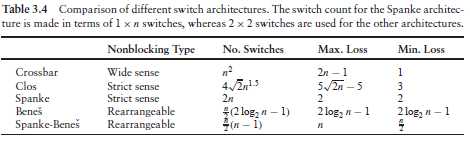
\includegraphics[width=378.1pt]{images/image151.png}
\end{center}
\end{frame}

\begin{frame}[shrink=20,t]{Αρχιτεκτονική Crossbar}
\begin{itemize}
\item Μία σύνδεση μπορεί να χρειάζονται από 1 μέχρι 2\textit{n}-1 switch για να ικανοποιηθεί.
\item Οι συνδέσεις μεταξύ των switch δεν χρειάζεται να τέμνονται.
\item wide sense non-blocking.
\item πρώτα διατρέχουμε ως προς γραμμές και μετά ως προς στήλες!
\end{itemize}
\begin{center}
\setlength{\unitlength}{0.000043pt}
\begin{picture}(3857652,3519155)
\put(0,0){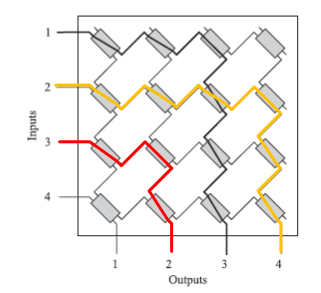
\includegraphics[width=164.4pt]{images/image153.png}}
\put(2627094,2435442){\footnotesize \shortstack{!!!!}}
\end{picture}
\end{center}
\end{frame}

\begin{frame}[shrink=20,t]{Αρχιτεκτονική Clos}
\begin{itemize}
\item στο πρώτο στάδιο χρησιμοποιούμε \textit{k} switch \textit{m}\ensuremath{\times}\textit{p} θυρών το καθένα.
\item στο δεύτερο στάδιο χρησιμοποιούμε \textit{p} switch διαστάσεων \textit{k}\ensuremath{\times}\textit{k}.
\item το τρίτο στάδιο είναι το ίδιο με το πρώτο.
\item Αν \textit{p}\ensuremath{\ge}2\textit{m}-1 τότε ο μεταγωγέας είναι \textit{strictly non-blocking. }
\item Για p=2m-1 χρειαζόμαστε
\begin{itemize}
\item \textit{m}\ensuremath{\times}(2\textit{m}-1) μεταγωγείς 2\ensuremath{\times}2 για κάθε έναν από τους \textit{m}\ensuremath{\times}\textit{p}\textit{ }μεταγωγείς.
\item \textit{k}$^{\text{2}}$ μεταγωγείς 2\ensuremath{\times}2 για κάθε έναν από τους μεταγωγείς \textit{k}\ensuremath{\times}\textit{k}\textit{.}
\item Σύνολο: 2\textit{km}(2\textit{m}-1)+(2\textit{m}-1)\textit{k}$^{\text{2}}$ μεταγωγείς 2\ensuremath{\times}2.
\item Αριθμός εισόδων και εξόδων \textit{n}=\textit{km}\textit{.}
\item Ελάχιστος αριθμός 2x2 μεταγωγών όταν \textit{m}\ensuremath{\cong}(\textit{n}/2)$^{\text{1/2}}$ oπότε έχουμε 4\ensuremath{\times}(2)$^{\text{1/2}}$\textit{n}$^{\text{3/2}}$-4\textit{n }μεταγωγείς
\end{itemize}
\end{itemize}
\begin{center}
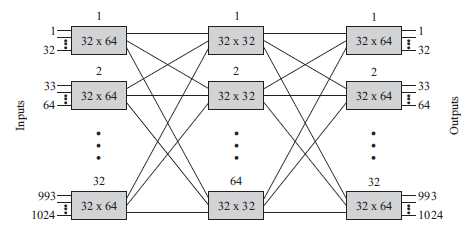
\includegraphics[width=310.0pt]{images/image154.png}
\end{center}
\end{frame}

\begin{frame}[shrink=10,t]{Spanke}
\begin{itemize}
\item ιδανική όταν χρησιμοποιούμε τεχνολογίες που μας δίνουνε απευθείας 1\ensuremath{\times}\textit{n} switch.
\end{itemize}
\begin{center}
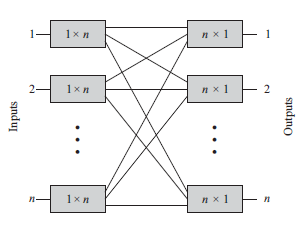
\includegraphics[width=199.4pt]{images/image155.png}
\end{center}
\end{frame}

\begin{frame}[shrink=10,t]{Bene\v{s}}
\begin{center}
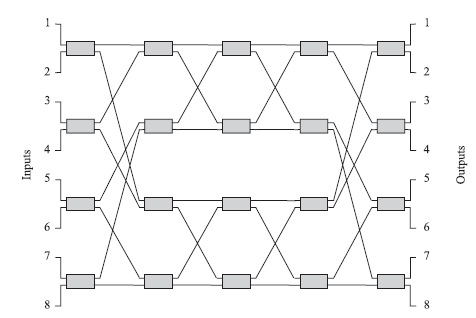
\includegraphics[width=291.9pt]{images/image156.png}
\end{center}
\end{frame}

\begin{frame}[shrink=10,t]{Απαιτήσεις}
\begin{center}
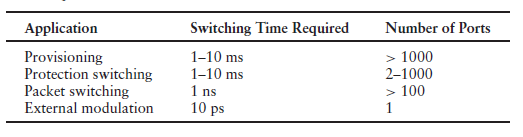
\includegraphics[width=378.1pt]{images/image157.png}
\end{center}
\end{frame}

\begin{frame}[shrink=10,t]{Τεχνολογίες Μεταγωγέων}
\begin{center}
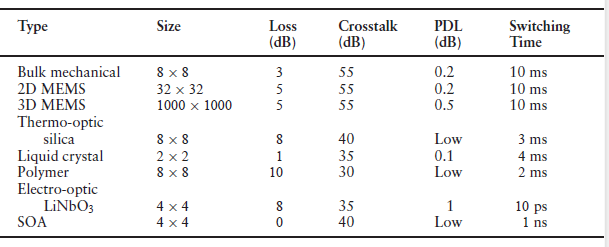
\includegraphics[width=378.1pt]{images/image158.png}
\end{center}
\end{frame}

\begin{frame}[shrink=10,t]{Μηχανικοί Μεταγωγείς}
\begin{itemize}
\item Μηχανικοί διακόπτες σε διακριτή μορφή (bulk mechanical switches).
\begin{itemize}
\item ένας καθρέφτης κινείται μηχανικά εντός ή εκτός του οπτικού μονοπατιού.
\item εναλλακτικά μία ίνα κάμπτεται  ή πιέζεται μηχανικά αλλάζοντας το συντελεστή σύζευξης κ σε έναν συζεύκτη.
\item γενικά χαμηλές απώλειες εισαγωγής, χαμηλές απώλειες λόγω πόλωσης, χαμηλή διαφωνία και χαμηλό κόστος.
\item χρησιμοποιούν την crossbar αρχιτεκτονική \ensuremath{\Rightarrow} πρόβλημα με την ομοιομορφία των απωλειών.
\item χρόνος μεταγωγής: μερικά ms.
\item μηχανική διάταξη \ensuremath{\Rightarrow} προβλήματα αντοχής στο χρόνο.
\end{itemize}
\end{itemize}
\end{frame}

\begin{frame}[shrink=20,t]{Micro-Electro-Mechanical System (MEMS)}
\begin{itemize}
\item Πρόκειται για διατάξεις με πολύ μικρές διαστάσεις που κατασκευάζονται πάνω σε υπόστρωμα πυριτίου.
\item συνήθως είναι μικροί καθρέφτες από πυρίτιο με διαστάσεις (\textasciitilde{}100μm εώς mm).
\item Στο ίδιο υπόστρωμα μπορούμε να αναπτύξουμε πολλούς καθρέφτες με σχετικά απλές τεχνικές.
\item Επίσης με ηλεκτρονικό τρόπο μπορούμε να αλλάξουμε την θέση των καθρεφτών (ηλεκτρομαγνητικά, ηλεκτροστατικά, πιεζοηλεκτρικά).
\item two-state pop-up mirror (ή 2D mirror):
\begin{itemize}
\item οριζόντια θέση (το φως περνάει).
\item κάθετη θέση (το φως ανακλάται).
\item χρησιμοποιείται για την σύνθεση  μέχρι και 32\ensuremath{\times}32 μεταγωγέων.
\item ψηφιακός έλεγχος (on/off)
\end{itemize}
\end{itemize}
\begin{center}
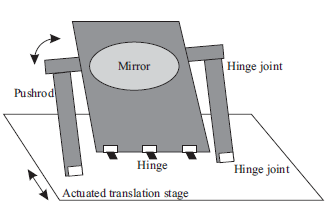
\includegraphics[width=238.2pt]{images/image159.png}
\end{center}
\end{frame}

\begin{frame}[shrink=20,t]{Micro-Electro-Mechanical System (MEMS)}
\begin{itemize}
\item Analog beam steering mirror
\begin{itemize}
\item Δυσκολότερος έλεγχος (αναλογικός)
\item Μπορεί να χρησιμοποιηθεί στην υλοποίηση μεταγωγέων 1\ensuremath{\times}\textit{n}\textit{.}\textit{ }
\end{itemize}
\end{itemize}
\begin{center}
\setlength{\unitlength}{0.000050pt}
\begin{picture}(4629150,3019425)
\put(0,0){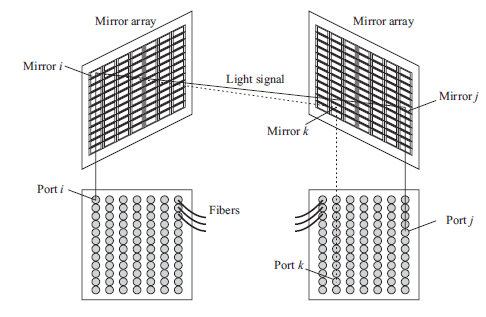
\includegraphics[width=230.0pt]{images/image161.png}}
\end{picture}
\end{center}
\centering\footnotesize Οι τρισδιάστατες τεχνολογίες MEMs επιτρέπουνε την υλοποίηση μεγάλων οπτικών μεταγωγέων με 256 ακόμα και 1000 θύρες\par
\end{frame}

\begin{frame}[shrink=20,t]{Μεταγωγείς υγρών κρυστάλλων}
\begin{itemize}
\item Υγροί κρύσταλλοι:
\begin{itemize}
\item Ανάλογα με το αν εφαρμόζεται ή όχι ηλεκτρικό πεδίο ο υγρός κρύσταλλος μπορεί ή όχι να στρέψει την πόλωση του φωτός.
\item Η αρχή λειτουργίας του μεγαγωγέα υγρού κρυστάλλου είναι παρόμοια με του απομονωτή.
\item Ο έλεγχος δεν χρειάζεται να είναι ψηφιακός. Αν είναι αναλογικός τότε μπορούμε να υλοποιήσουμε με την ίδια διάταξη έναν μεταβλητό εξασθενητή (variable optical attenuator – VOA).
\item Χρόνος μεταγωγής: μερικά ms.
\item Δυνατότητα ολοκλήρωσης \ensuremath{\Rightarrow} μικρό κόστος και μεγάλος όγκος παραγωγής
\end{itemize}
\end{itemize}
\begin{center}
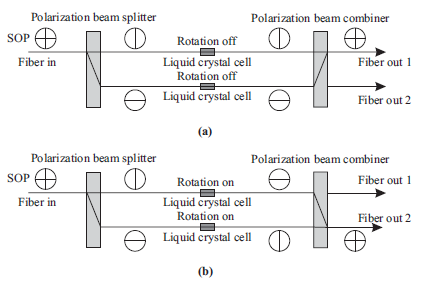
\includegraphics[width=215.5pt]{images/image162.png}
\end{center}
\end{frame}

\begin{frame}[shrink=10,t]{Ηλεκτροοπτικοί μεταγωγείς}
\begin{itemize}
\item Στην ουσία είναι ένας εξωτερικός διαμορφωτής που χρησιμοποιεί LiNbO
\item Μπορεί επομένως να χρησιμοποιεί διάταξη συζεύκτη ή διάταξη MZI.
\item Πλεονεκτήματα:
\begin{itemize}
\item Πολύ γρήγοροι, χρόνος μεταγωγής: ns
\item Μπορούν να ολοκληρωθούν πολλοί μεταγωγείς σε ένα υπόστρωμα.
\end{itemize}
\item Μειονεκτήματα:
\begin{itemize}
\item Σχετικά υψηλές απώλειες εισαγωγής
\item Σχετικά υψηλή PDL – polarization dependent loss
\item Κόστος: γενικά πιο ακριβοί από μηχανικά switch.
\end{itemize}
\end{itemize}
\end{frame}

\begin{frame}[t]{Θερμοοπτικοί Μεταγωγείς}
\begin{itemize}
\item Είναι MZI τα οποία αποτελούνται από υλικό του οποίου ο δείκτης διάθλασης εξαρτάται ισχύρα από την θερμοκρασία.
\item Επομένως αλλάζοντας την θερμοκρασία, αλλάζουμε το δ.δ. και επομένως την διαφορά δρόμου των δύο δρόμων του MZI.
\item Μπορούν να φτιαχτούν σε Si αλλά και από οργανικά υλικά.
\item Ωστόσο έχουνε υψηλή διαφωνία και σχετικά αργούς τρόπους μεταγωγής.
\end{itemize}
\end{frame}

\begin{frame}[shrink=10,t]{Ενισχυτές ημιαγωγού (ως μεταγωγείς)}
\begin{itemize}
\item Ο SOA μπορεί να παίξει το ρόλο ενός μεταγωγέα:
\begin{itemize}
\item όταν τροφοδοτείται με τάση αφήνει το σήμα να περνάει και μάλιστα το ενισχύει.
\item όταν δεν τροφοδοτείται με τάση τότε απλά απορροφά την οπτική ισχύ του σήματος.
\end{itemize}
\item Πλεονεκτήματα:
\begin{itemize}
\item γενικά παρέχει πολύ μεγάλους λόγους σβέσης.
\item χρόνος μεγαγωγής: μερικά ns.
\item δυνατότητα ολοκλήρωσης με συζεύκτες, κτλ ώστε να υλοποιηθούν μεγαλύτερα switch.
\end{itemize}
\item Μειονεκτήματα:
\begin{itemize}
\item είναι ακριβό component.
\item έχει δυσκολίες στον έλεγχο της πόλωσης.
\end{itemize}
\end{itemize}
\end{frame}

\begin{frame}[shrink=20,t]{Ηλεκτρονικοί μεταγωγείς}
\begin{itemize}
\item Μέχρι τώρα ασχοληθήκαμε με καθαρά οπτικούς (all-optical) μεταγωγείς.
\item Στην πράξη όμως πολύ συχνά με τον όρο “οπτικό” μεταγωγέα εννοούμε έναν μεταγωγέα που χρησιμοποιεί ηλεκτρονικά για την δρομολόγηση των σημάτων.
\item Ένας μεγάλος ηλεκτρονικός μεταγωγέας χρησιμοποιεί συνήθως την αρχιτεκτονική Clos και έναν αριθμό μικρότερων μεταγωγέων.
\item Υπάρχουν δύο τρόποι να γίνει η μεταγωγή:
\begin{itemize}
\item χωρίζουμε τα σήματα των 2.5Gb/s και 10Gb/s σε μικρότερα (π.χ. 51Mb/s). Αυτό έχει νόημα όταν θέλουμε να δρομολογήσουμε απευθείας αυτά τα μικρότερα σήματα.
\item η άλλη προσέγγιση είναι να κάνουμε απευθείας την μεταγωγή με ένα ηλεκτρονικό crossbar το οποίο υλοποιείται με ένα ολοκληρωμένο οπτικό κύκλωμα (IC).
\end{itemize}
\item Πρόβλημα ισχύος:
\begin{itemize}
\item ένα 64\ensuremath{\times}64 IC καταναλώνει μέχρι και 25W και χρειάζονται περίπου 100 τέτοια IC για να υλοποιήσουμε ένα 1024\ensuremath{\times}1024 switch\ensuremath{\Rightarrow}25kW.
\item Σε αντίθεση ένα 3D MEM switch 1024\ensuremath{\times}1024 χρειάζεται 3kW.
\item Οι ηλεκτρονικοί μεταγωγείς χρειάζονται ψύξη.
\end{itemize}
\item Oταν πρέπει να συνδεθούνε μεταξύ τους πολλά ICs αυτό γίνεται συνήθως πάνω σε μία πλακέτα ή από πλακέτα σε πλακέτα.
\begin{itemize}
\item Είναι δύσκολο να βρεθούν ηλεκτρονικά interconnects που να υποστηρίζουν >2.5Gb/s σε αποστάσεις 5-6m.
\item Mπορούμε να χρησιμοποιήσουμε οπτικά interconnects που καταλανώνουνε μικρότερη ισχύ και έχουν εμβέλεια >100m.
\end{itemize}
\end{itemize}
\end{frame}

\begin{frame}[shrink=20,t]{Μετατροπείς μήκους κύματος}
\begin{itemize}
\item Ο μετατροπέας μήκους κύματος αλλάζει το μήκος κύματος ενός σήματος.
\item Χρειάζεται σε ένα δίκτυο WDM επειδή
\begin{itemize}
\item τα δεδομένα μπορεί να βρίσκονται σε ένα μήκος κύματος ακατάλληλο για μετάδοση (π.χ. αν εκπέμπονται αρχικά στο 1310nm τότε για να τα μεταφέρουμε σε ένα σύγχρονο δίκτυο θα πρέπει να τα φέρουμε στο 1550nm). Στην περίπτωση αυτή ο μετατροπέας μήκους κύματος ονομάζεται \textit{transponder}.
\item θέλουμε να βελτιώσουμε την χρήση των πόρων του δικτύου (δηλαδή των lightpaths).
\item στα όρια διαφορετικών δικτύων ενδεχομένως να χρειάζεται μετατροπή μήκους κύματος αν αυτά είναι διαχειρίσιμα μέσω διαφορετικών οντοτήτων που δεν συντονίζουν μεταξύ τους την κατανομή των μηκών κύματος.
\end{itemize}
\item Κατηγοριοποίηση μετατροπέων μήκους κύματος:
\begin{itemize}
\item fixed input, fixed output.
\item fixed input, variable output.
\item variable input, fixed output.
\item variable input, variable output.
\end{itemize}
\end{itemize}
\end{frame}

\begin{frame}[shrink=20,t]{Οπτικοηλεκτρονική Προσέγγιση}
\begin{itemize}
\item Regeneration + Reshaping + Retiming (3R)
\end{itemize}
\begin{center}
\setlength{\unitlength}{0.000065pt}
\begin{picture}(5534025,1685925)
\put(0,0){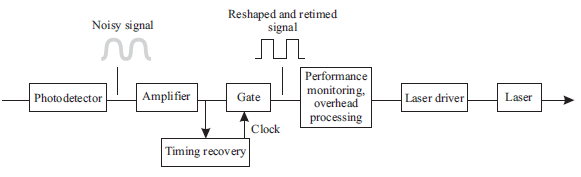
\includegraphics[width=358.2pt]{images/image163.png}}
\put(4483456,1685925){\footnotesize \shortstack{Regeneration (1R)}}
\put(425529,1685925){\footnotesize \shortstack{Regeneration + Reshaping (2R)}}
\end{picture}
\end{center}
\centering\footnotesize Το σήμα ανιχνεύεται και ως ένα σημείο αναγεννιέται (regeneration) εκπεμπόμενο σε ένα νέο μήκος κύματος. Συνήθως είναι variable input, fixed output.\par
\end{frame}

\begin{frame}[shrink=20,t]{Οπτικές Προσεγγίσεις: Gating (*)}
\begin{itemize}
\item Μειονεκτήματα:
\begin{itemize}
\item υψηλή ισχύ εισόδου για να συμβεί ικανοποιητικό CGM (\textasciitilde{}0dBm).
\item μικρός λόγος σβέσης εισόδου (\ensuremath{\le}10dB)
\item εκτός του cross gain υπάρχει και το cross phase που μπορεί να προκαλέσει σημαντική παραμόρφωση σήματος εξόδου.
\item Χρειάζεται φίλτρο για να “κόψει” το \textit{λ}$_{\text{\textit{p}}}$ στην έξοδο.
\end{itemize}
\end{itemize}
\medskip
\begin{itemize}
\item Βασίζεται σε Cross Gain Modulation (CGM) μέσα σε SOA.
\item υψηλό σήμα (bit “1”) στο \textit{λ}$_{\text{\textit{s }}}$\ensuremath{\Rightarrow} χαμηλό κέρδος \ensuremath{\Rightarrow} δεν ενισχύεται πολύ το σήμα στο \textit{λ}$_{\text{\textit{p}}}$.
\item ρυθμοί μέχρι 10Gb/s (το CGM είναι γρήγορο φαινόμενο)
\end{itemize}
\begin{center}
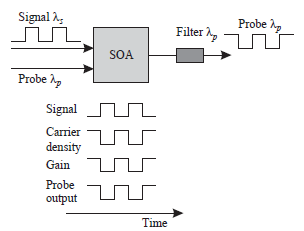
\includegraphics[width=197.4pt]{images/image166.png}
\end{center}
\end{frame}

\begin{frame}[shrink=10,t]{Οπτικές Προσεγγίσεις: Συμβολόμετρο (*)}
\begin{itemize}
\item Οι διαφορές φάσεις στον κάθε SOA λόγω XPM μετατρέπονται σε διαφορές πλάτους στο συμβολόμετρο.
\item Μικρότερη ισχύ, καλύτερος λόγος σβέσης
\end{itemize}
\begin{center}
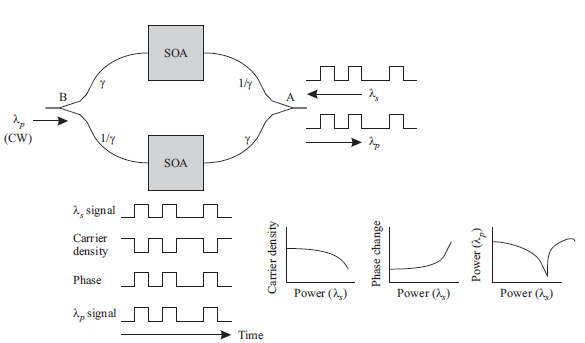
\includegraphics[width=255.8pt]{images/image167.png}
\end{center}
\end{frame}

\begin{frame}[shrink=10,t]{Οπτικές Προσεγγίσεις: FWM (*)}
\begin{center}
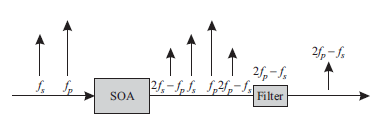
\includegraphics[width=378.1pt]{images/image168.png}
\end{center}
\end{frame}

\section[Διαμόρφωση]{Μέρος 3$^{\text{ο}}$: Διαμόρφωση και αποδιαμόρφωση οπτικών σημάτων}
\begin{frame}
\vfill
\begin{center}
{\Large\structure{Μέρος 3$^{\text{ο}}$: Διαμόρφωση και αποδιαμόρφωση οπτικών σημάτων}}
\end{center}
\vfill
\end{frame}

\begin{frame}[shrink=10,t]{Διαμόρφωση On/Off (OOK).}
\begin{center}
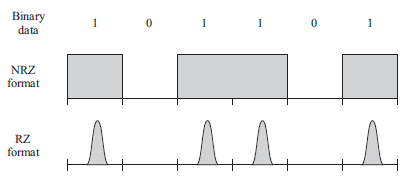
\includegraphics[width=378.1pt]{images/image169.png}
\end{center}
\end{frame}

\begin{frame}[shrink=20,t]{RZ και NRZ}
\begin{itemize}
\item Non-return to zero (NRZ): ο παλμός του “1” καταλαμβάνει \textbf{ολόκληρη} την διάρκεια του bit.
\begin{itemize}
\item αποδοτικότερη χρήση του φάσματος από το RZ.
\item μικρότερη ισχύ κορυφής σε σχέση με το RZ για να έχουμε την ίδια \textit{ενέργεια ανά }\textit{bit}.
\item Πρόβλημα στην περίπτωση διαδοχικών “1” \ensuremath{\Rightarrow} Χάνεται ο συγχρονισμός.
\end{itemize}
\item DC ισορροπία: όλες οι ακολουθίες bit που μπορούν να μεταδοθούν πρέπει να αντιστοιχούν στην ίδια μέση ισχύ.
\begin{itemize}
\item πιο εύκολη στρατηγική για το κατώφλι απόφασης στο δέκτη
\item \textit{line coding}: είναι ένας γραμμικός κώδικας που μετατρέπει k bit μηνύματος σε κωδικές λέξεις των n bits έτσι ώστε να έχουν DC ισορροπία και αρκετές μεταβάσεις. Παράδειγμα ο κώδικας (8,10) του Fibre Channel.
\item \textit{scrambling}: μετατρέπουμε απλά τα bit εισόδου (XOR με μία άλλη ακολουθία bit). Aποδοτικότερη χρήση φάσματος αλλά δεν είναι εγγυημένη η DC ισορροπία.
\end{itemize}
\item Στην πράξη:
\begin{itemize}
\item NRZ με ταχύτητες 155Mb/s έως 10Gb/s.
\item Line coding στο Gigabit Ethernet και στο Fibre Channel.
\item Το Scrambling είναι απλό και πολύ διαδεδομένο.
\end{itemize}
\end{itemize}
\end{frame}

\begin{frame}[shrink=20,t]{Διαμόρφωση σε υποφέρουσες}
\begin{itemize}
\item Η φέρουσα συχνότητα ενός σήματος στo λ=1550nm είναι η \textit{f}=\textit{c}/\textit{λ}\textit{\ensuremath{\cong}}2\ensuremath{\times}10$^{14}$Hz.
\item H πληροφορία αποτυπώνεται πάνω σε αυτή την συχνότητα, δηλαδή το σήμα είναι \textit{y}(\textit{t})=\textit{x}(\textit{t})cos(2π\textit{ft}).
\item Γιατί να μην διαμορφώσουμε το \textit{x}(\textit{t}) με παρόμοιο τρόπο; \textit{x}(\textit{t})=\textit{x}$_{\text{1}}$(\textit{t})cos(2π\textit{f}$_{\text{1}}$\textit{t})+…+\textit{x}$_{\text{\textit{N}}}$(\textit{t})cos(2π\textit{f}$_{\text{\textit{N}}}$\textit{t}).
\item Τα \textit{f}$_{\text{1}}$,..\textit{f}$_{\text{\textit{N}}}$ ονομάζονται υποφέρουσες συχνότητες.
\item Είναι ένας εύκολος τρόπος να πολυπλέκουμε (ηλεκτρονικά) πολλά μικρού ρυθμού σήματα \textit{x}$_{\text{1}}$(\textit{t}), … \textit{x}$_{\text{\textit{N}}}$(\textit{t}) σε ένα σήμα.
\item Χρησιμοποιείται:
\begin{itemize}
\item για μετάδοση αναλογικής τηλεόρασης και δεδομένων
\item στο μητροπολιτικό δίκτυο για την μετάδοση των δεδομένων πολλών χρηστών
\item για την παράλληλη μετάδοση καναλιών ελέγχου.
\end{itemize}
\end{itemize}
\end{frame}

\begin{frame}[shrink=10,t]{Φασματική Απόδοση}
\begin{itemize}
\item Φασματική απόδοση είναι ο λόγος του ρυθμού μετάδοσης προς το εύρος ζώνης του σήματος.
\item Μετριέται σε bit/s/Hz.
\item Θεωρητικά, χρησιμοποιώντας on/off keying (OOK), μπορούμε να μεταδώσουμε με φασματική απόδοση 1b/s/Hz.
\item Ωστόσο στην πράξη πετυχαίνουμε αποδόσεις τις τάξης 0.4b/s/Hz.
\item Μπορούμε να βελτιώσουμε την απόδοση χρησιμοποιώντας πιο εξελιγμένα συστήματα διαμόρφωσης από το ΟΟΚ.
\item Παράδειγμα είναι η διαμόρφωση duobinary που αυξάνει την απόδοση κατά 50\%, δηλαδή 0.6b/s/Hz.
\end{itemize}
\end{frame}

\begin{frame}[shrink=20,t]{Διαμόρφωση duobinary}
\begin{itemize}
\item Προσθέτουμε στην ακολουθία των bit μία καθυστερημένη έκδοση της ίδιας ακολουθίας.
\item Π.χ. αν είναι να μεταδώσουμε την (0,0,1,0,1,0,0,1,1,0) τότε προσθέτουμε σε αυτήν την (*,0,0,1,0,1,0,0,1,1) όπου * είναι η αρχική τιμή της ακολουθίας που την θεωρούμε 0.
\item Επομένως μεταδίδουμε την (0,0,1,1,1,1,0,1,2,1).
\item Έχουμε λοιπόν \textit{y}(\textit{nT})=\textit{x}(\textit{nT})+\textit{x}(\textit{nT}-\textit{T}) όπου \textit{T} είναι η διάρκεια ενός bit.
\item Στο δέκτη ανακατασκευάζουμε τα δείγματα ως \textit{z}(\textit{nT})=\textit{y}(\textit{nT})-\textit{z}(\textit{nT}-\textit{T}).
\end{itemize}
\begin{center}
$\displaystyle \begin{aligned}z(nT)&=y(nT)-z(nT-T)=y(nT)-y(nT-T)+z(nT-T)\\&=y(nT)-y(nT-T)+y(nT-2T)-z(nT-3T)\\&=y(nT)-y(nT-T)+y(nT-2T)-\dots+(-1)^{n-1}y(T)\\&=[x(nT)+x(nT-T)]-[x(nT-T)+x(nT-2T)]+\dots\\&=x(nT)\end{aligned}$\\[0.6ex]
\end{center}
\end{frame}

\begin{frame}[shrink=20,t]{Διαμόρφωση duobinary}
\begin{itemize}
\item Έχουμε διάδοση σφάλματος να συμβεί κάποιο λάθος στην αποκωδικοποίηση.
\item Για το λόγο αυτό αντί να κωδικοποιούμε το μήνυμα αυτό κάθε αυτό, κωδικοποιούμε τις αλλαγές των bit.
\item Έστω δηλαδή ότι θέλουμε να μεταδώσουμε την \textit{d}(\textit{nT})=(0,0,1,1,1,1,0,1,0,1). Τότε μεταδίδουμε την \textit{x}(\textit{nT})=(0,0,1,0,1,0,0,1,1,0).
\item Δηλαδή αν η \textit{d}(\textit{nT})=1 τότε κάνουμε μία αλλαγή στην \textit{x}(\textit{nT}) από 0 σε 1 ή το 1 σε 0. Στην ουσία \textit{x}(\textit{nT})=\textit{x}(\textit{nT}-\textit{T})\ensuremath{\times}\textit{d}(\textit{nT}).
\item Στο δέκτη μπορούμε να ανακτήσουμε την \textit{d}(\textit{nT}) από την ακολουθία \textit{e}(\textit{nT})=\textit{z}(\textit{nT})\ensuremath{\times}\textit{z}(\textit{nT}\textit{-T})
\item Απουσία θορύβου, \textit{e}(\textit{nT})=\textit{x}(\textit{nT})\ensuremath{\times}\textit{x}(\textit{nT}\textit{-T})=\textit{x}(\textit{nT})=[\textit{x}(\textit{nT}-\textit{T})\ensuremath{\times}\textit{d}(\textit{nT})]\ensuremath{\times}\textit{x}(\textit{nT}\textit{-T})=[\textit{x}(\textit{nT}-\textit{T})\ensuremath{\times}\textit{x}(\textit{nT}\textit{-T})]\ensuremath{\times}\textit{d}(\textit{nT})=0\ensuremath{\times}\textit{d}(\textit{nT})=\textit{d}(\textit{nT}).
\item Αν υποθέσουμε τώρα πως γίνεται ένα σφάλμα στην αποκωδικοποίηση οπότε \textit{z}(\textit{nT})=\textit{x}(\textit{nT})\ensuremath{\times}1. Επειδή το σφάλμα διαδίδεται, έχουμε \textit{z}(\textit{nT}\textit{+Τ})=\textit{x}(\textit{nT}\textit{+Τ})\ensuremath{\times}1. Ωστόσο όμως \textit{e}(\textit{nT})=\textit{z}(\textit{nT})\ensuremath{\times}\textit{z}(\textit{nT}\textit{-T})=\textit{ x}(\textit{nT})\ensuremath{\times}\textit{x}(\textit{nT}\textit{-T}).
\end{itemize}
\end{frame}

\begin{frame}[shrink=20,t]{Διαμόρφωση duobinary}
\begin{itemize}
\item Για να έχουμε φασματική απόδοση με την duobinary διαμόρφωση θα πρέπει να κωδικοποιήσουμε τις στάθμες (0,1,2) ως (-1,0,1).
\item Αυτό γίνεται με την βοήθεια ενός Mach-Zehnder διαμορφωτή.
\item Προσφέρεται μεγαλύτερη ανοχή από αλληλοπαρεμβολή συμβόλων.
\item Επίσης η ισχύς |\textit{Ε}(\textit{t})|$^{\text{2}}$ είναι η ίδια με ενός συστήματος NRZ. Επομένως το φάσμα της ισχύος είναι το ίδιο με ένα NRZ.
\end{itemize}
\begin{center}
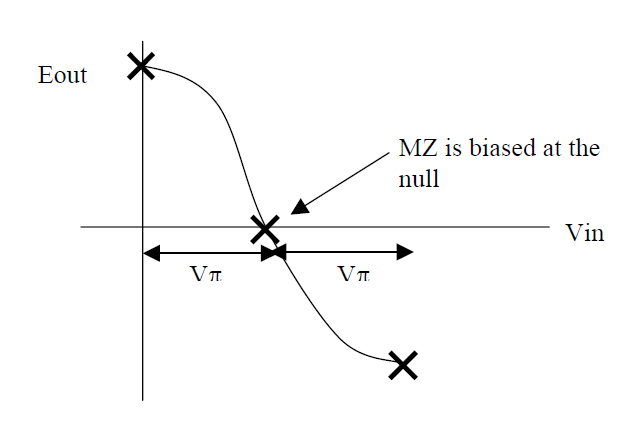
\includegraphics[width=155.6pt]{images/image171.png} 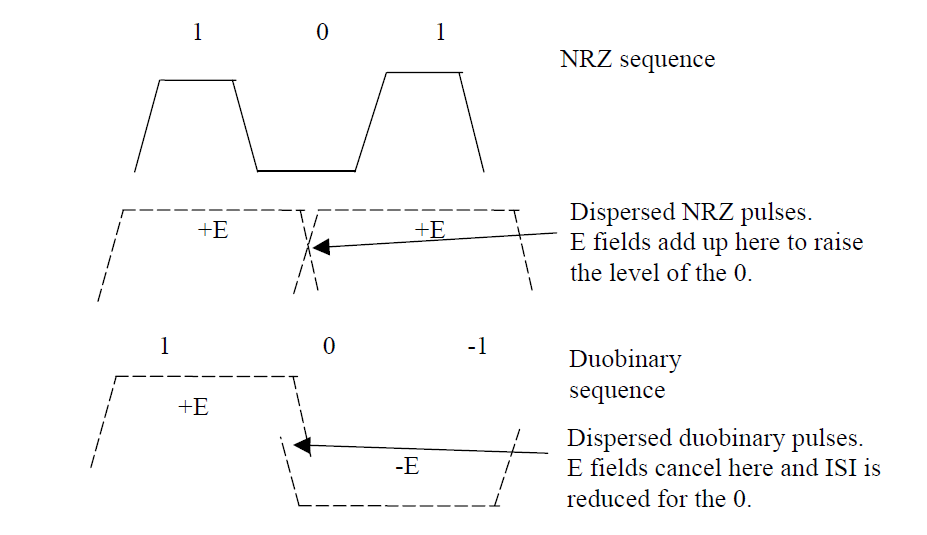
\includegraphics[width=182.7pt]{images/image172.png}
\end{center}
\end{frame}

\begin{frame}[shrink=10,t]{Διαμόρφωση πολλαπλών επιπέδων}
\begin{itemize}
\item Ένα πιο απλός τρόπος για την αύξηση της φασματικής απόδοσης είναι η χρήση περισσότερων επιπέδων.
\item Το ΟΟΚ έχει \textit{Μ}=2 στάθμες, μία για το 0 και μία για το 1.
\item Θα μπορούσαμε (στο ίδιο εύρος ζώνης) να κωδικοποιήσουμε το μήνυμα σε \textit{Μ}=4 στάθμες θεωρώντας δύο διαδοχικά bit.
\item Έτσι, “00”\ensuremath{\Rightarrow}0, “01”\ensuremath{\Rightarrow}1, “10”\ensuremath{\Rightarrow}2, “11”\ensuremath{\Rightarrow}3.
\item Η απόδοση πολλαπλασιάζεται επί log$_{\text{2}}$\textit{M.}
\item Ωστόσο, η εφαρμογή τέτοιων σχημάτων είναι σχετικά περιορισμένη επειδή είναι δυσκολότερη η υλοποίηση του δέκτη.
\end{itemize}
\end{frame}

\begin{frame}[shrink=10,t]{Φώραση σημάτων}
\begin{center}
\setlength{\unitlength}{0.000048pt}
\begin{picture}(7478820,1571636)
\put(0,0){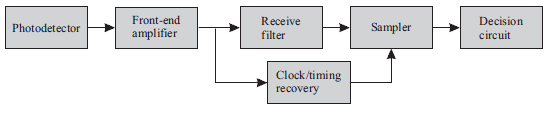
\includegraphics[width=358.2pt]{images/image173.png}}
\end{picture}
\end{center}
\centering\footnotesize Η ποιότητα της ανίχνευσης των bit στο δέκτη χαρακτηρίζεται από το Bit Error Rate (Ρυθμός Σφάλματος Bit). Στα οπτικά συστήματα μπορούμε να πετύχουμε τιμές του BER από 10$^{-9}$ έως 10$^{-15}$.\par
\end{frame}

\begin{frame}[shrink=20,t]{Διάγραμμα Ματιού}
\begin{itemize}
\item Το διάγραμμα ματιού συντίθεται από την υπέρθεση των κυματομορφών που λαμβάνουμε στα διαδοχικά bit.
\item Κάθετο άνοιγμα \ensuremath{\Rightarrow} δείχνει την επίδραση του θορύβου.
\item Οριζόντιο άνοιγμα \ensuremath{\Rightarrow} σφάλματα χρονισμού (ατελής ανάκτηση ρολογιού).
\end{itemize}
\begin{center}
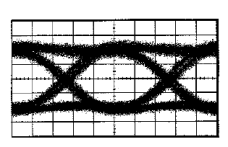
\includegraphics[width=82.2pt]{images/image174.png} 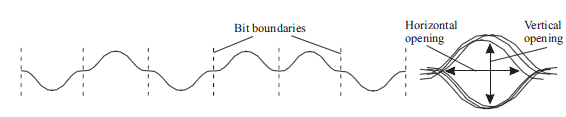
\includegraphics[width=256.1pt]{images/image175.png}
\end{center}
\end{frame}

\begin{frame}[shrink=20,t]{Ιδανικός Δέκτης}
\begin{itemize}
\item Ο ιδανικός δέκτης στην ουσία μετράει τα φωτόνια που λαμβάνει και αποφασίζει για το bit που λαμβάνει.
\item Καθόλου φωτεινή ισχύ\ensuremath{\Rightarrow}bit “0”
\item Ύπαρξη φωτεινή ισχύος\ensuremath{\Rightarrow}bit “1”
\item Πρόκειται για \textit{άμεση φώραση }(αποφασίζουμε για τα bit βασισμένοι σε πληροφορία της ισχύος του σήματος λήψης).
\item Ακόμα και απουσία άλλων θορύβων υπάρχει μία εγγενής τυχαιότητα στην κίνηση των φωτονίων.
\item Όταν η ισχύς του σήματος είναι ίση με \textit{P} έχουμε \textit{P}/\textit{hf} φωτόνια που ακολουθούν κατανομή Poisson (πιο σωστά οι αφίξεις ακολουθούν στατιστική Poisson).
\item Δηλαδή σε μία διάρκεια Τ=1/B όπου Β ο ρυθμός των bit η πιθανότητα να φτάσουνε \textit{n} φωτόνια είναι, exp(\ensuremath{-}\textit{PT}/\textit{hf})(\textit{PT}/\textit{hf})$^{\text{\textit{n}}}$/\textit{n}!
\item Στην περίπτωση όπου έχουμε bit 1 ο δέκτης μπορεί να αποφασίσει ότι πρόκειται για bit 0 με πιθανότητα (\textit{n}=0), exp(\ensuremath{-}\textit{PT}/\textit{hf}).
\item Οπότε αν τα bit είναι ισοπίθανα (δηλαδή εμφανίζονται με πιθανότητα \ensuremath{\tfrac{1}{2}}) , έχουμε BER=\ensuremath{\tfrac{1}{2}}exp(\ensuremath{-}\textit{PT}/\textit{hf})=\ensuremath{\tfrac{1}{2}}exp(-\textit{M}) όπου Μ είναι ο αριθμός των φωτονίων.
\item Κβαντικό όριο. Για BER=10$^{\text{-12,}}$ έχουμε \textit{M}=27 φωτόνια ανά bit.
\end{itemize}
\end{frame}

\begin{frame}[shrink=20,t]{Θερμικός θόρυβος}
\begin{itemize}
\item Οφείλεται στην τυχαία κίνηση των ηλεκτρονίων που υπάρχει πάντα σε μη μηδενικές θερμοκρασίες (\textit{Τ}>0$^{\text{ο}}$Κ).
\item Σε μία αντίσταση \textit{R }και σε θερμοκρασία \textit{T} η συνάρτηση αυτοσυσχέτισης του θορύβου είναι \textit{R}$_{\text{\textit{nn}}}$(τ)=<\textit{n}(\textit{t})\textit{n}(\textit{t}+\textit{τ})>=4\textit{k}$_{\text{\textit{B}}}$\textit{T}/\textit{R}$_{\text{\textit{L}}}$\textit{δ}(\textit{τ}) όπου δ(τ) είναι η συνάρτηση του Dirac.
\item Σε ένα εύρος ζώνης \textit{B}$_{\text{\textit{e}}}$ έχουμε διακύμανση (variance) εξαιτίας του θερμικού θορύβου, \textit{σ}$_{\text{th}}$$^{\text{2}}$=(4\textit{k}$_{\text{\textit{B}}}$\textit{T}/\textit{R}$_{\text{\textit{L}}}$)\textit{B}$_{\text{\textit{e}}}$.
\item Ορίζουμε την παράμετρο \textit{I}$_{\text{\textit{t}}}$ έτσι ώστε \textit{I}$_{\text{\textit{t}}}$$^{\text{2}}$=4\textit{k}$_{\text{\textit{B}}}$\textit{T}/\textit{R}\textit{, }οπότε \textit{σ}$_{\text{th}}$$^{\text{2}}$=\textit{I}$_{\text{\textit{t}}}$$^{\text{2}}$\textit{B}$_{\text{\textit{e}}}$\textit{.} Τυπικές τιμές είναι \textit{I}$_{\text{\textit{t}}}$=1pA/Ηz$^{\text{1/2}}$.
\item Το ηλεκτρικό εύρος ζώνης \textit{Β}$_{\text{\textit{e}}}$ συνήθως κυμαίνεται μεταξύ 1/(2\textit{Τ}) και 1/\textit{Τ}.
\item Πέρα από το ηλεκτρικό εύρος ζώνης, υπάρχει και το οπτικό εύρος ζώνης του δέκτη \textit{Β}$_{\text{\textit{ο}}}$. Συνήθως θέτουμε \textit{Β}$_{\text{\textit{ο}}}$=2\textit{Β}$_{\text{\textit{e}}}$.
\item Στην περίπτωση που ο δέκτης χρησιμοποιεί ηλεκτρονικό ενισχυτή, \textit{σ}$_{\text{th}}$$^{\text{2}}$=(4\textit{k}$_{\text{\textit{B}}}$\textit{T}/\textit{R}$_{\text{\textit{L}}}$)\textit{Β}$_{\text{\textit{e}}}$\textit{F}, όπου \textit{F} είναι η εικόνα θορύβου του ενισχυτή (3-5dB).
\end{itemize}
\end{frame}

\begin{frame}[shrink=20,t]{Θόρυβος βολής (shot)}
\begin{itemize}
\item Εξαιτίας της τυχαίας άφιξης των φωτονίων, τα ηλεκτρόνια έχουνε και αυτά μία τυχαιότητα.
\item Μπορούμε να θεωρήσουμε ότι το φωτόρευμα δίνεται από την σχέση \textit{Ι}=\textit{Ι}+\textit{i}$_{\text{\textit{s}}}$.
\item To is μπορούμε να θεωρήσουμε πως είναι τυχαία Gaussian διαδικασία με μηδενική μέση τιμή και αυτοσυσχέτιση \textit{R}(\textit{τ})=\textit{σ}$_{\text{shot}}$$^{\text{2}}$\textit{δ}(\textit{τ}).
\item Στην περίπτωση των δεκτών pin έχουμε
\begin{itemize}
\item \textit{Ι}\textit{=RP}
\item \textit{σ}$_{\text{shot}}$$^{\text{2}}$\textit{=2e}\textit{Ι}\textit{B}$_{\text{\textit{e}}}$\textit{.}
\end{itemize}
\item Στην περίπτωση των δεκτών APD,
\begin{itemize}
\item \textit{Ι}\textit{=R}$_{\text{APD}}$\textit{P=}\textit{G}$_{\text{\textit{m}}}$\textit{RP}\textit{.}
\item \textit{σ}$_{\text{shot}}$$^{\text{2}}$=2\textit{eG}$_{\text{\textit{m}}}$$^{\text{2}}$\textit{F}$_{\text{\textit{A}}}$(\textit{G}$_{\text{\textit{m}}}$)\textit{RPB}$_{\text{\textit{e}}}$.
\item \textit{F}$_{\text{\textit{A}}}$(\textit{G}$_{\text{\textit{m}}}$)=\textit{k}$_{\text{\textit{A}}}$\textit{G}$_{\text{\textit{m}}}$+(1-\textit{k}$_{\text{\textit{A}}}$)(2$^{-1}$/\textit{G}$_{\text{\textit{m}}}$), όπου ο συντελεστής \textit{k}$_{\text{\textit{A}}}$ είναι ο λόγος ιονισμού (\textit{k}$_{\text{\textit{A}}}$<1 για το Si στα 0.8μm ενώ \textit{k}$_{\text{\textit{A}}}$=0.7 για το InGaAs στο 1.3μm και 1.55μm).
\end{itemize}
\item Η συνολική διακύμανση θορύβου είναι \textit{σ}$^{\text{2}}$=\textit{σ}$_{\text{shot}}$$^{\text{2}}$+\textit{σ}$_{\text{th}}$$^{\text{2}}$.
\end{itemize}
\end{frame}

\begin{frame}[shrink=20,t]{Δέκτης με οπτική προενίσχυση}
\begin{itemize}
\item Οι δέκτες με οπτική προενίσχυση προσπαθούν να αυξήσουν την ισχύ του σήματος ως προς την ισχύ του θερμικού θορύβου και του θορύβου shot.
\item Δυστυχώς όμως υπάρχει και ο θόρυβος ενισχυμένης αυθόρμητης εκπομπής (amplified spontaneous emission – ASE).
\item Είναι οπτικός θόρυβος που παρουσιάζεται στην έξοδο του ενισχυτή. Εμφανίζεται και στις δύο πολώσεις του φωτός και
\item Σε κάθε συνιστώσα πόλωσης η ισχύς του θορύβου είναι \textit{P}$_{\text{\textit{N}}}$=\textit{n}$_{\text{sp}}$\textit{hf}(\textit{G}-1)\textit{B}$_{\text{\textit{o}}}$=\textit{P}$_{\text{\textit{n}}}$\textit{Β}$_{\text{\textit{ο}}}$ .H συνολική ισχύς θορύβου είναι 2\textit{P}$_{\text{\textit{N}}}$.
\item H παράμετρος nsp είναι μία παράμετρος που καθορίζει πόσο ισχυρή είναι η αναστροφή πληθυσμών στον ενισχυτή.
\begin{itemize}
\item Ιδανικά \textit{n}$_{\text{sp}}$=1 (πλήρης αναστροφή).
\item Στην πράξη \textit{n}$_{\text{\textit{sp}}}$=3 έως 5.
\end{itemize}
\end{itemize}
\end{frame}

\begin{frame}[shrink=20,t]{Δέκτης με οπτική προενίσχυση}
\begin{itemize}
\item Στην περίπτωση του δέκτη με προενίσχυση ο δέκτης βλέπει το πεδίο \textit{Ε}$_{\text{\textit{s}}}$(\textit{t})+\textit{E}$_{\text{\textit{n}}}$(\textit{t}) και το φωτόρευμα είναι ανάλογο του |\textit{Ε}$_{\text{\textit{s}}}$+\textit{E}$_{\text{\textit{n}}}$|$^{\text{2}}$=|\textit{E}$_{\text{\textit{s}}}$|$^{\text{2}}$+2Re\{\textit{E}$_{\text{\textit{s}}}$\textit{E}$_{\text{\textit{n}}}$$^{\text{*}}$\}+|\textit{Ε}$_{\text{\textit{n}}}$|$^{\text{2}}$.
\item Έχουμε δηλαδή μίξη σήματος με θόρυβο και μίξη θορύβου με θόρυβο.
\begin{itemize}
\item \textit{Ι}=\textit{RGP}, όπου \textit{G} είναι το κέρδος του ενισχυτή.
\item \textit{σ}$_{\text{th}}$$^{\text{2}}$\textit{=I}$_{\text{\textit{t}}}$$^{\text{\textit{2}}}$\textit{B}$_{\text{\textit{e}}}$\textit{.}
\item \textit{σ}$_{\text{shot}}$$^{\text{2}}$=2\textit{eR}(\textit{GP}+\textit{P}$_{\text{\textit{n}}}$(\textit{G}-1)\textit{B}$_{\text{\textit{o}}}$)\textit{B}$_{\text{\textit{e}}}$.
\item \textit{σ}$_{\text{sig-sp}}$$^{\text{2}}$=4\textit{R}$^{\text{2}}$\textit{GPP}$_{\text{\textit{n}}}$(\textit{G}-1)\textit{B}$_{\text{\textit{e}}}$.
\item \textit{σ}$_{\text{sp-sp}}$$^{\text{2}}$=2\textit{R}$^{\text{2}}$[\textit{P}$_{\text{\textit{n}}}$(\textit{G}-1)]$^{\text{2}}$(2\textit{B}$_{\text{\textit{o}}}$-\textit{B}$_{\text{\textit{e}}}$)\textit{B}$_{\text{\textit{e}}}$.
\end{itemize}
\item Πηλίκο σήμα προς θόρυβο:
\begin{itemize}
\item πριν τον ενισχυτή, SNR$_{\text{\textit{i}}}$=(\textit{RP})$^{\text{2}}$/(2\textit{R}e\textit{PB}$_{\text{\textit{e}}}$).
\item μετά τον ενισχυτή (θεωρώντας ότι ο sig-sp είναι ο ισχυρότερος) SNR$_{\text{o}}$=(\textit{RGP})$^{\text{2}}$/(4\textit{R}$^{\text{2}}$\textit{PG}(\textit{G}-1)\textit{n}$_{\text{sp}}$\textit{hfB}$_{\text{\textit{e}}}$).
\item εικόνα θορύβου \textit{F}$_{\text{\textit{n}}}$=SNR$_{\text{i}}$/SNR$_{\text{o}}$\ensuremath{\cong}2\textit{n}$_{\text{sp}}$.
\end{itemize}
\end{itemize}
\end{frame}

\begin{frame}[shrink=20,t]{Υπολογισμός του BER}
\begin{itemize}
\item Πως αποφασίζει ένας δέκτης; Συγκρίνει το ρεύμα που λαμβάνεται \textit{Ι} με μία τιμή κατωφλίου \textit{I}$_{\text{th}}$.
\begin{itemize}
\item Αν \textit{I}\ensuremath{\ge}\textit{I}$_{\text{th}}$, τότε θεωρεί ότι μεταδόθηκε “1”.
\item Αν \textit{Ι}<\textit{Ι}$_{\text{th}}$, τότε θεωρεί ότι μεταδόθηκε “0”.
\end{itemize}
\item Παρουσία θορύβου, ο δέκτης μπορεί να κάνει σφάλμα.
\item Θεωρούμε πως ο θόρυβος είναι Gaussian, δηλαδή ακολουθεί κατανομή \textit{f}(\textit{i}$_{\text{\textit{n}}}$)=1/[\textit{σ}(2π)$^{\text{1/2}}$]exp(\ensuremath{-}\textit{i}$_{\text{\textit{n}}}$$^{\text{2}}$/2/\textit{σ}$^{\text{2}}$).
\item P[\textit{i}|\textit{j}] = πιθανότητα ο δέκτης να αποκωδικοποιήσει \textit{i} ενώ ο πομπός έχει στείλει \textit{j}.
\item H πιθανότητα σφάλματος (δηλαδή το BER) είναι BER=P[1]P[0|1]+P[0]P[1|0].
\item Στην περίπτωση ισοπίθανων bit έχουμε P[0]=P[1]=\ensuremath{\tfrac{1}{2}}, επομένως BER=\ensuremath{\tfrac{1}{2}}(P[0|1]+P[1|0]).
\end{itemize}
\end{frame}

\begin{frame}[shrink=20,t]{Υπολογισμός του BER}
\begin{center}
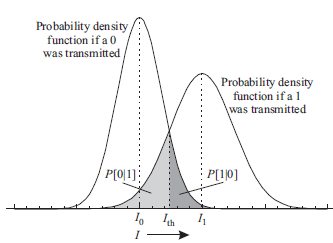
\includegraphics[width=267.2pt]{images/image179.png}
\end{center}
\begin{center}
$\displaystyle P[0|1]=\frac{1}{\sigma_{1}\sqrt{2\pi}}\int\limits_{-\infty}^{I_{th}}dx\,e^{-(x-I_{1})^{2}/(2\sigma_{1}^{2})}=Q\left(\frac{I_{1}-I_{th}}{\sigma_{1}}\right)$\\[0.6ex]
$\displaystyle Q(x)=\frac{1}{\sqrt{2\pi}}\int\limits_{x}^{\infty}dy\,e^{-y^{2}/2}$\\[0.6ex]
$\displaystyle P[1|0]=\frac{1}{\sigma_{0}\sqrt{2\pi}}\int\limits_{I_{th}}^{+\infty}dx\,e^{-(x-I_{0})^{2}/(2\sigma_{0}^{2})}=Q\left(\frac{I_{th}-I_{0}}{\sigma_{0}}\right)$\\[0.6ex]
\end{center}
\end{frame}

\begin{frame}[shrink=20,t]{Βέλτιστο Κατώφλι}
\begin{itemize}
\item Βέλτιστο κατώφλι \ensuremath{\Rightarrow} ελάχιστο BER
\item Θα πρέπει η παράγωγος του BER ως προς το \textit{I}$_{\text{th}}$ να είναι μηδέν, dBER/d\textit{Ι}$_{\text{th}}$=0.
\item Μπορούμε να δείξουμε ότι το βέλτιστο κατώφλι και η αντίστοιχη ελάχιστη πιθανότητα σφάλματος είναι:
\end{itemize}
\begin{center}
$\displaystyle I_{\mathrm{opt}}=\frac{\sigma_{0}I_{1}+\sigma_{1}I_{0}}{\sigma_{1}+\sigma_{0}}$\\[0.6ex]
$\displaystyle \mathrm{BER}_{\mathrm{opt}}=Q\left(\frac{I_{1}-I_{0}}{\sigma_{1}+\sigma_{0}}\right)$\\[0.6ex]
\end{center}
\end{frame}

\begin{frame}[shrink=20,t]{Ευαισθησία του δέκτη}
\begin{itemize}
\item Πόση ισχύς χρειάζεται ώστε να πετύχουμε μία ορισμένη πιθανότητα σφάλματος BER$_{\text{\textit{t}}}$?
\item Έστω ότι BER$_{\text{\textit{t}}}$=\textit{Q}(\textit{γ}). Π.χ.
\begin{itemize}
\item για BER$_{\text{\textit{t}}}$=10$^{-12}$ έχουμε \textit{γ}\ensuremath{\cong}7.
\item για BER$_{\text{\textit{t}}}$=10$^{\text{-}}$$^{\text{9}}$ έχουμε \textit{γ}\ensuremath{\cong}6.
\end{itemize}
\item Αν θεωρήσουμε πως \textit{P}$_{\text{0}}$=0 (δηλαδή η ισχύς που λαμβάνεται όταν μεταδίδουμε “0” είναι ίση με 0), τότε
\begin{itemize}
\item \textit{Ι}$_{\text{0}}$=\textit{RP}$_{\text{0}}$=0.
\item \textit{I}$_{\text{1}}$=\textit{RP}$_{\text{1}}$\textit{.}
\item \textit{γ}=(\textit{Ι}$_{\text{1}}$-\textit{Ι}$_{\text{0}}$)/(\textit{σ}$_{\text{1}}$+\textit{σ}$_{\text{0}}$)=\textit{Ι}$_{\text{1}}$/(\textit{σ}$_{\text{1}}$+\textit{σ}$_{\text{0}}$).
\item H μέση ισχύς είναι \textit{P}$_{\text{avg}}$=\textit{P}$_{\text{1}}$/2.
\item \textit{P}$_{\text{avg}}$=(\textit{σ}$_{\text{0}}$+σ$_{\text{1}}$)\textit{γ}/(2\textit{R}).
\end{itemize}
\item Αυτή είναι η ευαισθησία του δέκτη, δηλαδή η μέση ισχύς ανά bit που πρέπει να λάβει ώστε να πετύχει πιθανότητα σφάλματος BERt.
\item O αριθμός των φωτονίων \textit{Μ} είναι \textit{M}=2\textit{P}$_{\text{avg}}$/(\textit{hfB}) όπου \textit{B} είναι ο ρυθμός των bit.
\end{itemize}
\end{frame}

\begin{frame}[shrink=20,t]{Ευαισθησία του δέκτη}
\begin{itemize}
\item Σε κάθε περίπτωση υπολογίζουμε την ισχύ θορύβου του “1” και την ισχύ θορύβου του “0”.
\begin{itemize}
\item Δέκτης pin, \textit{σ}$_{\text{1}}$$^{\text{2}}$=\textit{σ}$_{\text{th}}$$^{\text{2}}$+\textit{σ}$_{\text{sh}}$$^{\text{2}}$, \textit{σ}$_{\text{0}}$$^{\text{2}}$=\textit{σ}$_{\text{th}}$$^{\text{2}}$, \textit{σ}$_{\text{th}}$$^{\text{2}}$=(4\textit{k}$_{\text{\textit{B}}}$\textit{T}/\textit{R})\textit{FB}$_{\text{\textit{e}}}$\textit{, }\textit{σ}$_{\text{sh}}$$^{\text{2}}$\textit{=4eRP}$_{\text{avg}}$\textit{B}$_{\text{\textit{e}}}$\textit{.}
\item Δέκτης APD, \textit{σ}$_{\text{1}}$$^{\text{2}}$=\textit{σ}$_{\text{th}}$$^{\text{2}}$+\textit{σ}$_{\text{sh}}$$^{\text{2}}$, \textit{σ}$_{\text{0}}$$^{\text{2}}$=\textit{σ}$_{\text{th}}$$^{\text{2}}$, \textit{σ}$_{\text{th}}$$^{\text{2}}$=(4\textit{k}$_{\text{\textit{B}}}$\textit{T}/\textit{R})\textit{FB}$_{\text{\textit{e}}}$\textit{, }4\textit{eG}$_{\text{\textit{m}}}$$^{\text{2}}$\textit{F}$_{\text{\textit{A}}}$(\textit{G}$_{\text{\textit{m}}}$)\textit{RP}$_{\text{avg}}$\textit{B}$_{\text{\textit{e}}}$\textit{.}
\item Προενισχυμένος δέκτης:
\end{itemize}
\end{itemize}
\textit{σ}$_{\text{sig-sp}}$$^{\text{2}}$=8\textit{R}$^{\text{2}}$\textit{GP}$_{\text{avg}}$\textit{n}$_{\text{sp}}$(\textit{G}-1)\textit{hfB}$_{\text{\textit{e}}}$.\par
\textit{I}$_{\text{1}}$=2\textit{GRP}$_{\text{avg}}$.\par
Θεωρούμε \textit{σ}$_{\text{0}}$<<\textit{σ}$_{\text{1}}$, \textit{n}$_{\text{sp}}$=1, \textit{Β}$_{\text{\textit{e}}}$=\textit{B}/2 μεγάλο κέρδος, \textit{G}(\textit{G}-1)\ensuremath{\cong}G$^{\text{2}}$, άρα \textit{γ}=2\textit{GRP}$_{\text{avg}}$/(\textit{σ}$_{\text{1}}$+\textit{σ}$_{\text{0}}$)\ensuremath{\cong}\textit{P}$_{\text{avg}}$/2/\textit{hf}\textit{/B} =\textit{M}/2\textit{.}\par
επομένως BER=\textit{Q}([\textit{M/2}]$^{\text{1/2}}$), 98 φωτόνια για 10$^{-12}$.\par
\end{frame}

\begin{frame}[shrink=10,t]{Ευαισθησία δέκτη}
\begin{center}
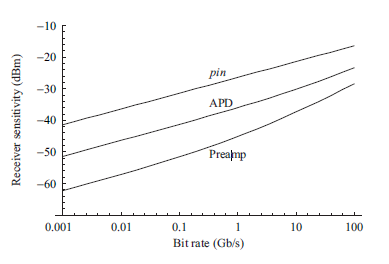
\includegraphics[width=287.3pt]{images/image182.png}
\end{center}
\end{frame}

\begin{frame}[shrink=20,t]{Σύμφωνη Φώραση}
\begin{itemize}
\item Στα παραπάνω το b είναι 0 ή 1 ανάλογα με το ποιο bit μεταδώσαμε.
\item Στην περίπτωση ομόδυνης φώρασης (\textit{f}$_{\text{\textit{c}}}$=\textit{f}$_{\text{LO}}$):
\begin{itemize}
\item \textit{I}$_{\text{1}}$=\textit{R}[\textit{P}+\textit{P}$_{\text{LO}}$+2(\textit{P}$_{\text{LO}}$\textit{P})$^{\text{1/2}}$].
\item \textit{Ι}$_{\text{0}}$=\textit{RP}$_{\text{LO}}$.
\item Στην περίπτωση μεγάλης PLO επιβιώνει μόνο ο θόρυβος shot, \textit{σ}$_{\text{1}}$$^{\text{2}}$=2\textit{eI}$_{\text{1}}$\textit{B}$_{\text{\textit{e}}}$, \textit{σ}$_{\text{0}}$$^{\text{2}}$=2\textit{eI}$_{\text{0}}$\textit{B}$_{\text{\textit{e}}}$.
\item BER=\textit{Q}([\textit{RP}/2/\textit{e}/\textit{B}$_{\text{\textit{e}}}$]$^{\text{1/2}}$)=\textit{Q}(\textit{M}$^{\text{1/2}}$) αν θεωρήσουμε ότι \textit{B}$_{\text{\textit{e}}}$=\textit{B}/2.
\item 49 φωτόνια (τα μισά σε σχέση με τον προενισχυμένο δέκτη) για BER=10$^{-12}$.
\end{itemize}
\end{itemize}
\begin{center}
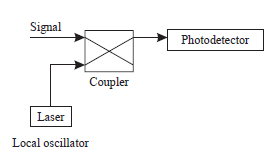
\includegraphics[width=264.2pt]{images/image184.png}
\end{center}
\begin{center}
$\displaystyle \begin{aligned}P_{r}(t)&=\left(\sqrt{bP}\cos(2\pi f_{c}t)+\sqrt{P_{\mathrm{LO}}}\cos(2\pi f_{\mathrm{LO}}t)\right)^{2}\\&=bP+P_{\mathrm{LO}}+2\sqrt{bPP_{\mathrm{LO}}}\cos\bigl(2\pi(f_{c}-f_{\mathrm{LO}})t\bigr)\end{aligned}$\\[0.6ex]
\end{center}
\end{frame}

\begin{frame}[shrink=10,t]{Σύμφωνη Φώραση}
\begin{itemize}
\item Πλεονεκτήματα:
\begin{itemize}
\item Καλύτερη ευαισθησία σε σχέση με ένα προενισχυμένο δέκτη άμεσης φώρασης (3~dB).
\item Δυνατότητα αποπολυπλεξίας καναλιών WDM αλλάζοντας την \textit{f}$_{\text{LO}}$ και χρησιμοποιώντας ένα ηλεκτρονικό φίλτρο.
\end{itemize}
\item Μειονεκτήματα:
\begin{itemize}
\item Ευαισθησία στην πόλωση. Υπάρχουν πιο πολύπλοκοι ωστόσο δέκτες οι οποίοι προσφέρουν αναισθησί από την πόλωση.
\item Ευαισθησία στο θόρυβο φάσης του τοπικού ταλανωτή αλλά και του σήματος.
\item Γενικά πιο πολύπλοκη δομή από τους προενισχυμένους δέκτες.
\end{itemize}
\end{itemize}
\end{frame}

\begin{frame}[t]{Κώδικες Διόρθωσης και Ανίχνευσης Σφαλμάτων}
\begin{itemize}
\item Με την χρήση πλεονασμού (επιπλέον bit) προστατεύουμε τα bit του μηνύματος και μάλιστα μπορούμε να διορθώσουμε και λάθη.
\item \textit{Forward Error Correction} (FEC): διόρθωση σφαλμάτων στο δέκτη.
\item Στην περίπτωση του SONET/SDH αλλά και άλλων δικτύων επικοινωνιών κάνουμε \textit{ανίχνευση} και όχι \textit{διόρθωση} σφαλμάτων.
\item Στην περίπτωση αυτή στέλνουμε μία αίτηση για επανάληψη του μηνύματος (Automatic repeat request – ARQ).
\end{itemize}
\end{frame}

\begin{frame}[shrink=20,t]{Forward Error Correction - FEC}
\begin{itemize}
\item Χρησιμοποιούνται για μείωση του BER, κάτι που είναι σημαντικό για τα οπτικά συστήματα που πρέπει να λειτουργούν με πιθανότητες σφάλματος 10$^{-12}$.
\item Το FEC συνήθως δεν χρειάζεται σε απλά συστήματα ή σε συστήματα WDM με μεγάλη φασματική απόσταση.
\item Ωστόσο σε συστήματα WDM η χρήση FEC είναι επιτακτική πολλές φορές επειδή εξαιτίας της μη γραμμικότητας δεν μπορούμε να αυξήσουμε την ισχύ εκπομπής για να μειώσουμε το BER.
\item Υπόβαθρο του BER (\textit{BER floor}): Πολλές φορές, η ελάχιστη τιμή του BER περιορίζεται από θορύβους όπως η διαφωνία.
\item Το SNR της διαφωνίας θα δούμε ότι \textbf{δεν} εξαρτάται από την ισχύ των καναλιών και επομένως δεν μπορεί να μειωθεί εύκολα.
\item Οι κώδικες FEC μπορούν ωστόσο να μειώσουνε το BER περισσότερο.
\end{itemize}
\end{frame}

\section[Σχεδιασμός]{Σχεδιασμός Συστημάτων Μετάδοσης}
\begin{frame}
\vfill
\begin{center}
{\Large\structure{Σχεδιασμός Συστημάτων Μετάδοσης}}
\end{center}
\vfill
\end{frame}

\begin{frame}[shrink=10,t]{Μοντέλο ενός συστήματος WDM}
\begin{itemize}
\item Μας ενδιαφέρει να υπολογίσουμε
\begin{itemize}
\item Την πιθανότητα σφάλματος (BER).
\item Το περιθώριο ισχύος (σε dB) για να πέσει το BER σε μία συγκεκριμένη τιμή (π.χ. 10$^{-9}$ ή 10$^{-15}$).
\end{itemize}
\end{itemize}
\begin{center}
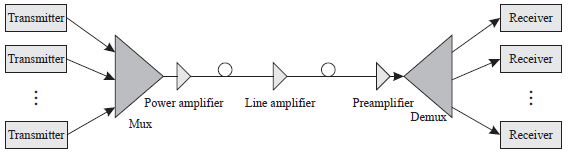
\includegraphics[width=338.3pt]{images/image185.png}
\end{center}
\end{frame}

\begin{frame}[shrink=10,t]{Μεγέθη που μας ενδιαφέρουν}
\begin{center}
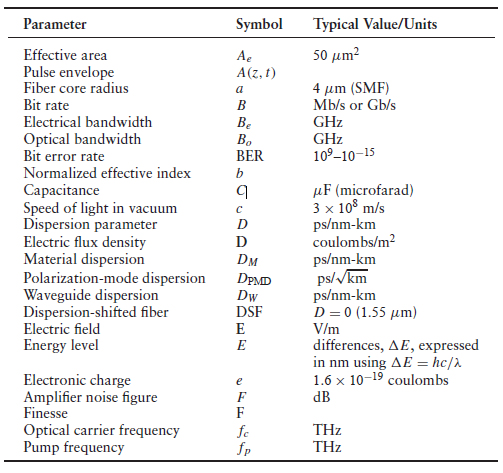
\includegraphics[width=207.4pt]{images/image186.png}
\end{center}
\end{frame}

\begin{frame}[shrink=10,t]{Μεγέθη που μας ενδιαφέρουν}
\begin{center}
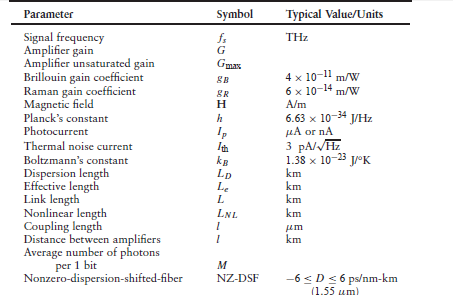
\includegraphics[width=204.6pt]{images/image187.png} 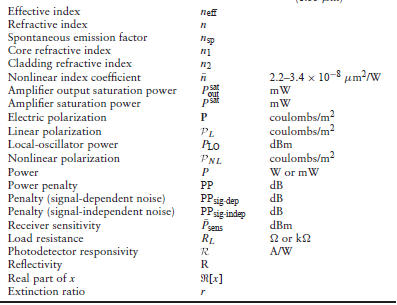
\includegraphics[width=173.5pt]{images/image188.png}
\end{center}
\end{frame}

\begin{frame}[shrink=20,t]{Power penalty (Ποινή ισχύος )}
\begin{itemize}
\item Μπορούμε να χαρακτηρίσουμε την σημασία κάθε ενός παράγοντα με το power penalty.
\item Το power penalty (PP) είναι η επιπλέον ισχύς εκπομπής που πρέπει να εκπέμψουμε ώστε λαμβάνοντας υπόψη τον παράγοντα αυτό να πετύχουμε μία τιμή στόχο για το BER.
\item Εναλλακτικά μπορούμε να ορίσουμε το power penalty ως την επιβάρυνση που φέρνει ο παράγοντας στο όρισμα γ που χρησιμοποιούμε για τον υπολογισμό του BER.
\item Έστω δηλαδή ότι απουσία του παράγοντα έχουμε ισχύ λήψης \textit{P}$_{\text{1}}$,\textit{P}$_{\text{0}}$ για τα bit “1” και “0” αντίστοιχα και ισχύ θορύβου \textit{σ}$_{\text{1}}$ και \textit{σ}$_{\text{0}}$.
\item Επίσης, παρουσία του παράγοντα έχουμε ισχύ λήψης \textit{P}\textit{’}$_{\text{1}}$,\textit{P}\textit{’}$_{\text{0}}$ για τα bit “1” και “0” αντίστοιχα και ισχύ θορύβου \textit{σ’}$_{\text{1}}$ και \textit{σ’}$_{\text{0}}$.
\item Αν \textit{γ}=\textit{R}(\textit{P}$_{\text{1}}$-\textit{P}$_{\text{0}}$)/(\textit{σ}$_{\text{1}}$+\textit{σ}$_{\text{0}}$) και \textit{γ’}=\textit{R}(\textit{P}\textit{’}$_{\text{1}}$-\textit{P}\textit{’}$_{\text{0}}$)/(\textit{σ’}$_{\text{1}}$+\textit{σ’}$_{\text{0}}$), τότε PP=\ensuremath{-}10log10(\textit{γ}’/\textit{γ}).
\end{itemize}
\end{frame}

\begin{frame}[shrink=20,t]{Πομπός}
\begin{itemize}
\item Υπάρχουν διάφορες παράμετροι που καθορίζουν τον πομπό:
\begin{itemize}
\item Ισχύ εκπομπής, λόγος σβέσης, χρόνος ανόδου και καθόδου για τους παλμούς που παράγονται, είδος διαμόρφωσης, επίπεδο καταστολής τρόπων, σταθερότητα μήκος κύματος και ακρίβεια.
\end{itemize}
\item Ισχύ εκπομπής:
\begin{itemize}
\item για DFB η ισχύς είναι περίπου από 1mW εώς 10mW.
\item Με χρήση οπτικής ενίσχυσης μπορεί να έχουμε και 50mW ισχύ εκπομπής.
\item Το άνω όριο τίθεται από τα μη γραμμικά φαινόμενα και διάφορες οδηγίες προστασίας.
\end{itemize}
\item Λόγος σβέσης:
\begin{itemize}
\item \textit{P}$_{\text{avg}}$=(\textit{P}$_{\text{1}}$+\textit{P}$_{\text{0}}$)/2=(\textit{P}$_{\text{1}}$+\textit{P}$_{\text{1}}$\textit{/r})/2 \ensuremath{\Rightarrow} \textit{P}$_{\text{1}}$=2\textit{rP}$_{\text{avg}}$/(\textit{r}+1) και \textit{P}$_{\text{0}}$=2\textit{P}$_{\text{avg}}$/(\textit{r}+1).
\item \textit{P}$_{\text{1}}$-\textit{P}$_{\text{0}}$=2(\textit{r}-1)\textit{P}$_{\text{avg}}$/(\textit{r}+1).
\item Στην περίπτωση θορύβου που δεν εξαρτάται από την ισχύ του σήματος (π.χ. θερμικός) έχουμε PP=-10log$_{\text{10}}$( [\textit{r}-1]/[\textit{r}+1] ).
\item Στα παραπάνω θεωρήσαμε ότι τα δύο συστήματα, (ιδανικό \textit{r}=\ensuremath{\infty}) και (μη ιδανικό \textit{r} πεπερασμένο) έχουν την ίδια μέση ισχύ εκπομπής.
\end{itemize}
\end{itemize}
\end{frame}

\begin{frame}[shrink=20,t]{Δέκτης}
\begin{itemize}
\item Η πιο σημαντική παράμετρος είναι η ευαισθησία, δηλαδή η οπτική ισχύς που χρειάζεται για να πετύχουμε μία τιμή-στόχο BER.
\item Συνήθως την υπολογίζουμε (ή την μετρούμε πειραματικά) για ένα BER=10$^{-12}$.
\item Επίσης μας ενδιαφέρει πόση είναι η ανώτερη ισχύ που μπορεί να προσπέσει στην είσοδο του δέκτη (overload parameter).
\end{itemize}
\begin{center}
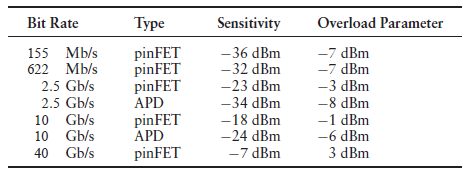
\includegraphics[width=338.3pt]{images/image189.png}
\end{center}
\end{frame}

\begin{frame}[shrink=20,t]{Οπτικοί ενισχυτές: Κόρος ισχύος}
\begin{itemize}
\item Οι EDFA προσφέρουν σημαντική ενίσχυση σε ένα εύρος ζώνης 35nm. Ωστόσο:
\begin{itemize}
\item Εισάγεται θόρυβος (ASE).
\item Το κέρδος εξαρτάται από την ισχύ εκπομπής.
\item Το κέρδος εξαρτάται από την συχνότητα.
\end{itemize}
\item Ο κόρος του κέρδους περιγράφεται από την εξίσωση \textit{G}=1+\textit{P}$_{\text{sat}}$/\textit{P}$_{\text{in}}$\textit{ln}(\textit{G}$_{\text{max}}$/\textit{G}).
\item \textit{P}$_{\text{sat}}$ είναι η ισχύς κόρου εισόδου.
\item Ισχύς κόρου εξόδου \textit{P}$_{\text{sout}}$ είναι η ισχύς εξόδου που λαμβάνουμε όταν το κέρδος έχει πέσει κατά 3~dB.
\item \textit{G}$_{\text{max}}$/2=1+\textit{P}$_{\text{sat}}$/\textit{P}$_{\text{in}}$ln2 \ensuremath{\Rightarrow} \textit{P}$_{\text{in}}$\ensuremath{\cong}(\textit{G}$_{\text{max}}$/2)$^{\text{-1}}$(\textit{ln}2)Psat \ensuremath{\Rightarrow} \textit{P}$_{\text{sout}}$=\textit{P}$_{\text{sat}}$(ln2).
\item Σε πρακτικά συστήματα έχουμε \textit{P}$_{\text{sout}}$ από 10dBm μέχρι 20dBm.
\end{itemize}
\end{frame}

\begin{frame}[shrink=10,t]{Εξίσωση συχνοτικής απόκρισης ενός EDFA}
\begin{itemize}
\item Είναι σημαντική στην περίπτωση συστημάτων WDM που αποτελούνται από διαδοχικούς ενισχυτές.
\item Οφείλεται στο ότι το κέρδος του ενισχυτή εξαρτάται από το μήκος κύματος, \textit{G}=\textit{G}(\textit{λ}).
\item Έτσι μικρόμεταβολές (π.χ. κατά 1dB/στάδιο) παρουσιάζονται ενισχυμένες (π.χ. 10dB μετά από δέκα στάδια).
\item Οι EDFA έχουν σχετικά ομαλό κέρδος στην περιοχή των 1545nm-1560nm. Ωστόσο δεν συμβαίνει το ίδιο στην περιοχή 1530nm-1545nm.
\item Εξίσωση (ομαλοποίηση) φασματικής απόκρισης.
\begin{itemize}
\item Χρήση αρχικής παραμόρφωσης (κάθε κανάλι με διαφορετική ισχύ).
\item Εξίσωση σε κάθε στάδιο (π.χ. με χρήση φίλτρων διηλεκτρικών στρωμάτων και φράγματα Bragg).
\end{itemize}
\end{itemize}
\end{frame}

\begin{frame}[shrink=20,t]{Ενισχυτές σε σειρά}
\begin{itemize}
\item Θεωρούμε πως για κάθε στάδιο το κέρδος είναι κοινό όπως και η ισχύς εξόδου.
\item Ισχύς στην έξοδο σε κάθε στάδιο: \textit{P}$_{\text{out}}$=\textit{P}$_{\text{out}}$exp(-\textit{al})\textit{G}+2\textit{P}$_{\text{\textit{n}}}$\textit{B}$_{\text{0}}$(\textit{G}-1)= ισχύς στην είσοδο εξασθενημένη εξαιτίας των απωλειών και ενισχυμένη εξαιτίας του ενισχυτή + θόρυβος ASE.
\item Κέρδος ενισχυτή: \textit{G}=1+\textit{P}$_{\text{sat}}$/[\textit{P}$_{\text{out}}$exp(-\textit{al})]ln[\textit{G}$_{\text{max}}$/\textit{G}].
\item Δύο εξισώσεις με δύο αγνώστους (G,\textit{P}$_{\text{out}}$).
\item Σε μία πιο απλή προσέγγιση ας απαιτήσουμε \textit{G}=exp(-\textit{al}).
\item Τότε η ισχύς του οπτικού θορύβου θα είναι \textit{P}$_{\text{noise}}$=2\textit{P}$_{\text{\textit{n}}}$\textit{B}$_{\text{0}}$(\textit{G}-1)\textit{L}/\textit{l}=2\textit{P}$_{\text{\textit{n}}}$\textit{B}$_{\text{0}}$(\textit{e}$^{\text{-}}$$^{\text{\textit{al}}}$-1)\textit{L}/\textit{l.}
\item Δεδομένου του OSNR (οπτικό SNR) που θέλουμε να πετύχουμε, απαιτούμε η ισχύς με την οποία εκπέμπεται το σήμα (και επομένως με την οποία λαμβάνεται αφού \textit{G}=exp(-\textit{al}) να είναι: \textit{P}\ensuremath{\ge}(OSNR)\textit{P}$_{\text{noise}}$.
\end{itemize}
\begin{center}
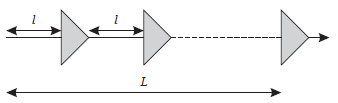
\includegraphics[width=338.3pt]{images/image190.png}
\end{center}
\end{frame}

\begin{frame}[shrink=10,t]{Απόσταση ενισχυτών και ισχύς εκπομπής}
\begin{center}
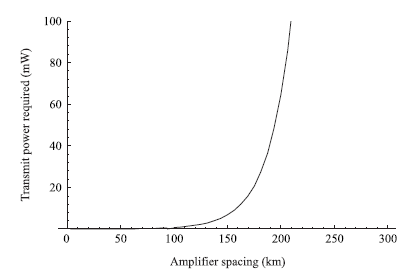
\includegraphics[width=285.5pt]{images/image191.png}
\end{center}
\end{frame}

\begin{frame}[shrink=20,t]{Ποινή ισχύος στην περίπτωση τοπικής ενίσχυσης}
\begin{itemize}
\item Από το προηγούμενο διάγραμμα: μικρή ισχύ εκπομπής \ensuremath{\Rightarrow} μικρό spacing ενισχυτών.
\item Ισχύς θορύβου: \textit{l}=ln\textit{G}/\textit{a} άρα: \textit{P}$_{\text{noise}}$=2\textit{LP}$_{\text{\textit{n}}}$B$_{\text{0}}$\textit{a}(\textit{G}-1)/ln\textit{G}.
\item Ελάχιστη τιμή θορύβου όταν \textit{G}\ensuremath{\Rightarrow}1 οπότε (\textit{G}\ensuremath{-}1)/ln\textit{G}\ensuremath{\Rightarrow}1.
\item Επομένως ο θόρυβος ενισχύεται κατά (\textit{G}\ensuremath{-}1)/ln\textit{G}\textit{ }σε σχέση με την κατανεμημένη ενίσχυση (\textit{G}\ensuremath{\Rightarrow}1, \textit{l}\ensuremath{\Rightarrow}0).
\item Αν θεωρήσουμε πως έχουμε την ίδια ισχύ εκπομπής P ενώ μεταβάλλουμε το l τότε βλέπουμε πως το OSNR μεταβάλλεται σύμφωνα με το (\textit{G}\ensuremath{-}1)/ln\textit{G}\textit{.}
\item Άρα έχουμε ποινή ισχύος (\textit{G}\ensuremath{-}1)/ln\textit{G}\textit{.}
\item Οι ενισχυτές Raman επομένως μπορούνε να μειώσουν τον συνολικό θόρυβο.
\end{itemize}
\end{frame}

\end{document}
